%%%%%%%%%%%%%%%%%%%%%%%%%%%%%%%%%%%%%%%%%%%%%%%%%%%%%%%%%%%%%%%%%%%%%%%%%%%%%%%%%%%%%%%%%%%%%%%%%%
%%%%%%%%%%% Document class and package options
%%%%%%%%%%%%%%%%%%%%%%%%%%%%%%%%%%%%%%%%%%%%%%%%%%%%%%%%%%%%%%%%%%%%%%%%%%%%%%%%%%%%%%%%%%%%%%%%%%
\documentclass[a4paper,12pt]{report}

\usepackage{graphicx} % graphics
\usepackage{subcaption} %sub-caption styles
\usepackage{placeins} % keep selected floats within their intended sections
\usepackage{amsmath} % equations and spacings
\usepackage{listings}
\usepackage{multicol}
\usepackage{enumerate}
\usepackage{fancyhdr}
\usepackage{lastpage}
\usepackage{longtable}
\usepackage{comment}
\usepackage{tikz} % block diagrams (methodology chapter)
\usepackage{rotating}   % for the sidewaystable environment
\usepackage{colortbl}   % for \cellcolor (the shaded milestone cells)
\usepackage{array}
\usetikzlibrary{arrows.meta, positioning, shapes.geometric, shapes.symbols, fit, backgrounds}

%%%%%%%%%%%%%%%%%%%%%%%%%%%%%%%%%%%%%%%%%%%%%%%%%%%%%%%%%%%%%%%%%%%%%%%%%%%%%%%%%%%%%%%%%%%%%%%%%%
% Include page set-up options
%%%%%%%%%%%%%%%%%%%%%%%%%%%%%%%%%%%%%%%%%%%%%%%%%%%%%%%%%%%%%%%%%%%%%%%%%%%%%%%%%%%%%%%%%%%%%%%%%%
\input{pagesetup.cfg}

%% ____Bibliography____%%
\usepackage[numbers,sort&compress]{natbib}
\usepackage{chapterbib}
\usepackage[breaklinks]{hyperref}
\hypersetup{colorlinks=true,citecolor=black,linkcolor=black,urlcolor=blue}

%% ____Nicely format and linebreak URLs in the bibliography (and elsewhere)____%%
\usepackage{url}
\def\UrlBreaks{\do\/\do\-\do\_\do\.}
\usepackage{breakurl}


\begin{document}

%%%%%%%%%%%%%%%%%%%%%%%%%%%%%%%%%%% The Front Matter %%%%%%%%%%%%%%%%%%%%%%%%%%%%%%%%%%%%
% Title Page

\thispagestyle{empty}

\begin{center}

\begin{center}
 
\includegraphics[width=2cm,keepaspectratio=true]{Front_matters/uor_logo.jpg}
 % uor_logo.jpg: 236x331 pixel, 72dpi, 8.33x11.68 cm, bb=0 0 236 331
\end{center}

\vspace{1.5cm}
\begin{huge}
%%%%%%%%%%%%%%%%%%%%%%%%%%%%%%%%%%%%%%%%%%%%%%%%%%%%
% Project title
%%%%%%%%%%%%%%%%%%%%%%%%%%%%%%%%%%%%%%%%%%%%%%%%%%%%
AI-Driven Self-Healing Security Framework for IoT Resilient Systems
%%%%%%%%%%%%%%%%%%%%%%%%%%%%%%%%%%%%%%%%%%%%%%%%%%%%
\end{huge} \\
\vspace{1cm}

\begin{normalsize}
An undergraduate project report submitted to the
\end{normalsize}\\
\vspace{1cm}

\begin{large}
Department of Electrical and Information Engineering\\
Faculty of Engineering\\
University of Ruhuna\\
Sri Lanka
\end{large}\\

\vspace{1cm}

\begin{normalsize}in partial fulfillment of the requirements for the \end{normalsize}\\
\vspace{1cm}

\begin{large}\textbf{Degree of the Bachelor of the Science of Engineering Honours}\end{large}\\

\vspace{1cm}
\begin{normalsize}by  \end{normalsize}
\vspace{1cm}

\begin{tabular}[h]{lll}
 %%%%%%%%%%%%%%%%%%%%%%%%%%%%%%%%%%%%%%%%%%%%%%%%%%%%%%%%%%
 % Names and Registration Numbers
 %%%%%%%%%%%%%%%%%%%%%%%%%%%%%%%%%%%%%%%%%%%%%%%%%%%%%%%%%%
 Dulkith G.L.M.	& - & 	EG/2021/4500\\
 Kalhara M.M.K.	& - & 	EG/2021/4593\\
 Samarasinghe N.A.C.V.	& - & 	EG/2021/4776\\
 Thashmika M.H.T.S. 	& - &	EG/2021/4826
 %%%%%%%%%%%%%%%%%%%%%%%%%%%%%%%%%%%%%%%%%%%%%%%%%%%%%%%%%%
\end{tabular}\\
\vspace{1cm}

%\date{June, 2009}
\vspace{1cm}

%%%%%%%%%%%%%%%%%%%%%%%%%%%%%%%%%%%%%%%%%%%%%%%%%%%%%
% Single supervisor
%%%%%%%%%%%%%%%%%%%%%%%%%%%%%%%%%%%%%%%%%%%%%%%%%%%%%%%
 .............................................. \\
Dr. Kushan Sudheera\\
(Supervisor)

\end{center}

%%%%%%%%%%%%%%%%%%%%%%%%%%%%%%%%%%%%%%%%%%%%%%%%%%%%%%%%%%%%%%%%%%%%%%%%%%%%%%%%%%%%%%%%%%%%%%%%%%
% END OF FILE
%%%%%%%%%%%%%%%%%%%%%%%%%%%%%%%%%%%%%%%%%%%%%%%%%%%%%%%%%%%%%%%%%%%%%%%%%%%%%%%%%%%%%%%%%%%%%%%%%%


\renewcommand{\thepage}{\roman{page}} % Start page numbering in roman

% Abstract, Acknowledgements, Preface, list of tables, list of figures and Acronyms

\chapter*{Abstract}

The Internet of Things (IoT) now underpins industrial control, smart-city, and healthcare infrastructure, yet its resource-constrained endpoints cannot host conventional security agents, exposing them to distributed denial-of-service (DDoS) attacks, botnet recruitment, and zero-day exploits~\cite{Antonakakis2017}. Existing defenses remain largely diagnostic: centralized detection adds latency, machine-learning classifiers behave as black boxes, and remediation still depends on manual intervention. This study proposes a two-tier self-healing framework coupling lightweight edge monitoring with cloud-based agentic intelligence. At the edge, a hybrid ensemble of a Gated Recurrent Unit (GRU) autoencoder and Support Vector Data Description (SVDD) captures temporal flow dependencies while preserving unsupervised anomaly boundaries, and a rolling risk score accumulates evidence across sliding windows and decays during benign activity, separating sustained attacks from transient jitter and suppressing false alarms. When the score signals a persistent threat, telemetry is offloaded to the cloud, where an XGBoost classifier identifies the attack vector and a SHapley Additive exPlanations (SHAP) module quantifies the contributing features~\cite{Lundberg2017}. These outputs feed a multi-agent large language model (LLM) core whose analytical, reporting, and orchestration agents interpret the attributions, generate forensic documentation, and consult a retrieval-augmented generation (RAG) knowledge base of device limitations, topology, and policy. The orchestrator issues executable healing actions. VLAN isolation, bandwidth throttling, or port blocking verifies them through the edge risk score in a closed loop, and escalates to operators only when automated options are exhausted. Experimental results show higher detection accuracy and lower false-positive rates than OC-SVM, autoencoder, and Isolation Forest baselines, with remediation dispatched within seconds.

\vspace{1em}
\noindent\textbf{\textit{Index Terms}}-Internet of Things (IoT) security, self-healing networks, anomaly detection, large language model (LLM) agents, distributed denial-of-service (DDoS) detection.

\addcontentsline{toc}{chapter}{Abstract} % add line to the table of contents


\chapter*{Acknowledgments}

We wish to express our sincere gratitude to our supervisor, Dr. Kushan Sudheera, for his invaluable guidance, continuous encouragement, and constructive feedback throughout the course of this project. His insights were instrumental in shaping both the technical direction and the presentation of this work.

We are also grateful to the Department of Electrical and Information Engineering, Faculty of Engineering, University of Ruhuna, for providing the academic environment, facilities, and resources necessary to carry out this project.

Finally, we extend our heartfelt thanks to our families and friends for their unwavering support and understanding throughout this undertaking.


\addcontentsline{toc}{chapter}{Acknowledgements} % add line to the table of contents

\begingroup
\hypersetup{linkcolor=black}
\tableofcontents
\addcontentsline{toc}{chapter}{Contents} % add line to the table of contents

\listoffigures
\addcontentsline{toc}{chapter}{List of Figures} % add line to the table of contents

\listoftables
\addcontentsline{toc}{chapter}{List of Tables} % add line to the table of contents
\endgroup

\chapter*{Acronyms}

\noindent \begin{longtable}{lcl}
AES	& - & Advanced Encryption Standard\\
AI	& - & Artificial Intelligence\\
API	& - & Application Programming Interface\\
ARP	& - & Address Resolution Protocol\\
AUC	& - & Area Under the Curve\\
C2	& - & Command and Control\\
CA	& - & Certificate Authority\\
CCTV	& - & Closed-Circuit Television\\
CPU	& - & Central Processing Unit\\
DDoS	& - & Distributed Denial-of-Service\\
DHCP	& - & Dynamic Host Configuration Protocol\\
DNS	& - & Domain Name System\\
DoS	& - & Denial-of-Service\\
DoT	& - & DNS over TLS\\
DVR	& - & Digital Video Recorder\\
F1	& - & F1-score\\
FAISS	& - & Facebook AI Similarity Search\\
FIN	& - & Finish (TCP flag)\\
FL	& - & Federated Learning\\
FN	& - & False Negative\\
FP	& - & False Positive\\
GPIO	& - & General Purpose Input/Output\\
GPU	& - & Graphics Processing Unit\\
GRU	& - & Gated Recurrent Unit\\
HTML	& - & HyperText Markup Language\\
HTTP	& - & Hypertext Transfer Protocol\\
HTTPS	& - & Hypertext Transfer Protocol Secure\\
ICMP	& - & Internet Control Message Protocol\\
IDS	& - & Intrusion Detection System\\
IID	& - & Independent and Identically Distributed\\
IIoT	& - & Industrial Internet of Things\\
IoT	& - & Internet of Things\\
IP	& - & Internet Protocol\\
IT	& - & Information Technology\\
JSON	& - & JavaScript Object Notation\\
LightGBM	& - & Light Gradient Boosting Machine\\
LIME	& - & Local Interpretable Model-agnostic Explanations\\
LLM	& - & Large Language Model\\
LSTM	& - & Long Short-Term Memory\\
MAC	& - & Media Access Control\\
MAS	& - & Multi-Agent System(s)\\
ML	& - & Machine Learning\\
MQTT	& - & Message Queuing Telemetry Transport\\
MSE	& - & Mean Squared Error\\
OAEP	& - & Optimal Asymmetric Encryption Padding\\
OC-SVM	& - & One-Class Support Vector Machine\\
PKCS	& - & Public-Key Cryptography Standards\\
PoE	& - & Power over Ethernet\\
PSK	& - & Pre-Shared Key\\
RAG	& - & Retrieval-Augmented Generation\\
RAM	& - & Random Access Memory\\
RMSprop	& - & Root Mean Square Propagation\\
RNN	& - & Recurrent Neural Network\\
ROC	& - & Receiver Operating Characteristic\\
RSA	& - & Rivest-Shamir-Adleman\\
RST	& - & Reset (TCP flag)\\
SCADA	& - & Supervisory Control and Data Acquisition\\
SDN	& - & Software-Defined Networking\\
SHA	& - & Secure Hash Algorithm\\
SHAP	& - & SHapley Additive exPlanations\\
SLM	& - & Small Language Model\\
SOC	& - & Security Operations Center\\
SSH	& - & Secure Shell\\
SVDD	& - & Support Vector Data Description\\
SYN	& - & Synchronize (TCP flag)\\
TCP	& - & Transmission Control Protocol\\
TF-IDF	& - & Term Frequency-Inverse Document Frequency\\
TLS	& - & Transport Layer Security\\
TTL	& - & Time To Live\\
UDP	& - & User Datagram Protocol\\
UI	& - & User Interface\\
UPnP	& - & Universal Plug and Play\\
UTC	& - & Coordinated Universal Time\\
VLAN	& - & Virtual Local Area Network\\
VoIP	& - & Voice over IP\\
VPN	& - & Virtual Private Network\\
WAF	& - & Web Application Firewall\\
XAI	& - & Explainable Artificial Intelligence\\
XGBoost	& - & Extreme Gradient Boosting\\
XSS	& - & Cross-Site Scripting\\
\end{longtable}

\addcontentsline{toc}{chapter}{Acronyms} % add line to the table of contents


%%%%%%%%%%%%%%%%%%%%%%% The main matters %%%%%%%%%%%%%%%%%%%%%%%%

\clearpage % close out the front matter's last page before renumbering
\renewcommand{\thepage}{\arabic{page}} % Start page numbering in arabic
\setcounter{page}{1} % start page numbering from 1

\chapter{Introduction}\label{cha:introduction}

\section{Background}

\subsection{Scale and Criticality of Contemporary IoT Deployment}

The Internet of Things has moved from an emerging technology to load-bearing digital infrastructure. IoT Analytics reports that the global installed base of connected IoT devices reached 18.5 billion at the end of 2024, a 12\% increase over 2023, and projects growth of a further 14\% to approximately 21.1 billion by the end of 2025, rising to an estimated 39 billion by 2030 at a compound annual growth rate of 13.2\% \cite{IoTAnalytics2025}. These figures deliberately exclude general-purpose computing devices such as laptops, smartphones and tablets, and therefore represent dedicated ``things'': industrial sensors, network video recorders, point-of-sale terminals, medical monitors, gateways and controllers \cite{IoTAnalytics2025}.

The significance of this expansion is not merely one of volume. IoT endpoints are increasingly embedded in systems where availability and integrity carry physical, rather than purely informational, consequences: industrial control loops, municipal utility telemetry, and clinical monitoring. A compromise in these settings is not confined to data loss; it can interrupt a process, degrade a safety function, or disable a service on which people depend. Consequently, the security posture of the endpoint population has become a question of operational resilience rather than of IT hygiene alone.

This shift is visible across sectors that have historically been treated as separate concerns by security research but that now share a common endpoint profile. Hospitals depend on networked infusion pumps, patient monitors and building-management sensors that were, in the great majority of cases, never designed to defend themselves against a network-borne adversary; water and power utilities depend on remote telemetry and control points scattered across a geographically dispersed footprint that cannot be physically hardened at scale; and manufacturing and logistics operators depend on programmable controllers and sensor meshes that must run continuously, often for a decade or longer, without a maintenance window in which security software could be patched or replaced. What unites these otherwise dissimilar sectors is that the endpoint, not the perimeter, is where risk now concentrates, and the endpoint is precisely the tier this project addresses.

\subsection{Resource Constraints and the Endpoint Security Gap}

The defining technical characteristic of IoT endpoints, and the root of their security problem, is severe resource constraint. RFC 7228 formalises this by defining three classes of constrained devices: Class 0 (much less than 10 KiB of RAM and much less than 100 KiB of code storage), Class 1 (approximately 10 KiB RAM and 100 KiB code storage), and Class 2 (approximately 50 KiB RAM and 250 KiB code storage) \cite{Bormann2014}. The same document observes that these boundaries move only slowly, because in the embedded space the gains from increased transistor density are typically reinvested in lower unit cost and lower power draw rather than in additional computing capability \cite{Bormann2014}.

This has a direct architectural consequence. Conventional endpoint security agents-host-based intrusion detection, endpoint detection and response, signature databases, and full cryptographic stacks-assume memory and processing budgets that are orders of magnitude beyond what these classes provide. Security must therefore be relocated: either to the network edge, where a gateway with modestly greater resources can observe device traffic passively, or to the cloud, where computation is effectively unbounded but latency and bandwidth are not. Neither location is sufficient in isolation, and the tension between them motivates the two-tier design presented in this report.

The constraint is not purely a matter of memory footprint; it is also a matter of energy and duty cycle. Many of the devices under discussion are battery-powered or energy-harvesting, and every millijoule spent on a cryptographic handshake, a signature update, or a background monitoring agent is a millijoule not spent on the device's primary sensing or actuation function. This creates a persistent incentive, at the manufacturing stage, to minimise on-device security logic in favour of battery life and unit cost, which in turn means that whatever security capability a fleet of such devices ends up with is largely determined by what can be added \emph{around} the device rather than \emph{on} it. That observation is the architectural premise underlying the edge-and-cloud split adopted in this project: rather than asking a Class 1 or Class 2 endpoint to run an anomaly detector, the detector is pushed one hop away, to a gateway that can absorb the computational and energy cost on the device's behalf.

The consequences of this gap are measurable. Forescout's fifth annual analysis of connected-device risk reported a 15\% year-over-year rise in average device risk score, from 7.73 in 2024 to 8.98 in 2025, with routers alone accounting for more than half of all devices carrying the most critical vulnerabilities \cite{Forescout2025}. The device types identified as riskiest within the IoT category-network video recorders, IP cameras, VoIP equipment, network-attached storage and point-of-sale systems-are, notably, long-standing rather than novel problems \cite{Forescout2025}. This persistence is itself informative: it suggests that the gap is not a temporary consequence of immature tooling that the market will eventually resolve, but a structural feature of how constrained devices are designed, procured and deployed, which is unlikely to close without a change in where the defensive workload is placed.

\subsection{The Evolving IoT Threat Landscape}

The canonical demonstration of aggregated IoT weakness remains the Mirai botnet. Antonakakis et al. document its growth to a peak of roughly 600,000 concurrent infections and its use against Krebs on Security, OVH and Dyn during late 2016; the initial attack on Krebs on Security exceeded 600 Gbps, sourced from what the authors describe as some of the least powerful hosts on the Internet \cite{Antonakakis2017}.

That capability has not diminished. In its Q3 2025 DDoS threat report, Cloudflare attributed a record attack peaking at 29.7 Tbps and 14.1 billion packets per second, lasting 69 seconds, to the Aisuru botnet-a TurboMirai-class IoT botnet estimated to comprise between one and four million compromised hosts, principally routers, CCTV cameras and DVR systems \cite{Cloudflare2025Q3, Kovacs2025}. Cloudflare reported mitigating 2,867 Aisuru attacks during 2025, of which 1,304 hyper-volumetric events occurred in Q3 alone \cite{Cloudflare2025Q3}. A subsequent attack peaking at 31.4 Tbps and lasting 35 seconds was reported in its Q4 2025 analysis \cite{Cloudflare2026Q4}. Comparing the 600 Gbps of 2016 with the tens of terabits per second of 2025 indicates roughly two orders of magnitude of growth in attainable attack volume drawn from the same class of endpoint.

Two properties of this traffic are directly relevant to defensive design. First, the attacks are short: Cloudflare observed that 71\% of HTTP-layer and 89\% of network-layer DDoS attacks concluded in under ten minutes \cite{Cloudflare2025Q3}. An incident that begins and ends inside ten minutes cannot be contained by a workflow that requires an analyst to receive an alert, interpret it, and manually configure a mitigation. Second, the compromised population is composed of devices that are, individually, unremarkable-which is precisely why per-device behavioural monitoring, rather than perimeter signature matching, is required to identify recruitment early.

The threat is not confined to volumetric botnet activity aimed outward at third parties; the same endpoint population is also the direct target of intrusions aimed at the operators who own it. An industry survey of 350 water and electricity operators across the United States and United Kingdom found that 62\% had been targeted by a cyberattack in the preceding year, and that 80\% of those had been targeted more than once; 54\% reported permanent corruption or destruction of data and operational systems as a result \cite{Semperis2025}. The same study attributed close to 60\% of the observed attacks to nation-state actors, and reported that compromised identity infrastructure, rather than the field devices themselves, was frequently the entry point-underscoring that the IoT and operational-technology layers of these organisations do not fail in isolation from the rest of the network, but are both a target and a launch point within a single, interconnected attack surface \cite{Semperis2025}. For a defensive architecture aimed at this endpoint population, this means that success cannot be judged solely by outward-facing metrics such as botnet participation; sustained, repeated targeting of the same device population, sometimes by well-resourced adversaries, must be treated as the baseline threat condition rather than the exceptional case.

\subsection{Limitations of Prevailing Detection and Response Practice}

Even where detection capability exists, the time to act on it has not improved. Mandiant's M-Trends 2025 reported a global median dwell time-the interval between initial compromise and detection-of 11 days for 2024, up from 10 days in 2023, against 205 days a decade earlier in 2014 \cite{Mandiant2025}. The following year's report recorded a further increase to 14 days for 2025, attributed in part to adversaries favouring edge devices such as routers, VPN appliances and firewalls, which typically ship without the logging depth that security teams expect from servers and endpoints \cite{Mandiant2026}. In other words, the very device class this project addresses is identified as a contributing blind spot.

The financial and operational consequences of this lag are quantifiable and, in physically consequential sectors, disproportionately severe. IBM's 2025 Cost of a Data Breach Report placed the global average cost of a breach at USD 4.44 million, the first year-on-year decline in five years, driven largely by faster containment through automated defences \cite{IBM2025}. Yet the same report found that healthcare organisations, which rely heavily on networked monitors, infusion pumps and building-management IoT, recorded the highest breach cost of any sector for the fifteenth consecutive year, with a breach lifecycle of 279 days-substantially longer than the 241-day global average-meaning that the sector with the greatest physical stakes is also the slowest to detect and contain an incident \cite{IBM2025}. This pattern is consistent with the broader argument of this report: where the consequences of compromise are most severe, the prevailing detection-to-response pipeline is least equipped to act quickly, which is the gap that motivates pushing detection and an initial remediation response down to the edge rather than depending exclusively on a centralised, human-mediated investigation.

Compounding this is the well-documented problem of alert fatigue, itself aggravated by a persistent shortage of qualified personnel to triage the alerts that detection systems do produce. Tariq et al., in a systematic review of the literature and industry practice, characterise alert fatigue as a socio-technical failure arising from alert volume, false-positive burden, tool fragmentation and analyst workload, and note survey evidence that a substantial majority of practitioners report burnout and increasing workload \cite{Tariq2025}. The 2025 SANS Detection and Response Survey correspondingly found that 73\% of organisations rank false positives as their foremost detection challenge \cite{SANS2025}. This is not simply a matter of insufficient headcount: the 2025 ISC2 Cybersecurity Workforce Study, drawing on responses from over sixteen thousand practitioners, found that only 34\% of organisations reported having the right level of cybersecurity staffing, and that budget constraints-rather than a lack of available candidates-had for the first time overtaken skills shortages as the primary driver of understaffed security teams \cite{ISC22025}. A detection system that raises an alarm on every transient traffic burst therefore does not merely produce noise; it actively erodes the trust and attention capacity of an already-stretched analyst population on which subsequent genuine alerts depend. This observation directly motivates the rolling, decaying risk score developed in Chapter \ref{cha:methodology}, and, more broadly, the decision to automate not only detection but an initial round of remediation, so that the framework's effectiveness does not depend on the availability of a human analyst at the moment an attack begins.

\subsection{Regulatory Pressure Toward Secure and Resilient Connected Products}

The policy environment has begun to codify what industry practice has not achieved voluntarily. The United Kingdom's consumer connectable product security regime, comprising Part 1 of the Product Security and Telecommunications Infrastructure Act 2022 together with the associated 2023 Regulations, came into force on 29 April 2024 and prohibits universal or easily guessable default passwords, requires a published point of contact for vulnerability reporting, and requires manufacturers to declare a minimum security update period \cite{UKPSTI2023}. At EU level, Regulation (EU) 2024/2847-the Cyber Resilience Act-entered into force on 10 December 2024, with vulnerability and incident reporting obligations applying from 11 September 2026 and full applicability from 11 December 2027; penalties for breaches of the essential requirements reach EUR 15 million or 2.5\% of worldwide annual turnover \cite{EU2024CRA}. In the United States, NIST IR 8259 and its companion core baseline set out foundational cybersecurity activities and device capabilities expected of IoT manufacturers \cite{Fagan2020}, complemented internationally by the ETSI EN 303 645 baseline for consumer IoT \cite{ETSI303645}.

Taken together, these instruments share a common structure: they legislate what a device must be capable of at the point of manufacture-strong authentication, a disclosed vulnerability-reporting channel, a defined update period-rather than how a device, or the network it sits within, should behave once that device has already been compromised. This is a deliberate and reasonable scope for product-safety regulation, but it leaves an operational gap precisely where this project is positioned. A newly manufactured device that fully satisfies the Cyber Resilience Act's essential requirements can still be recruited into a botnet once deployed, and none of the reviewed instruments mandate an automated detection-and-remediation capability at the network or gateway level. In this sense, regulation and the framework proposed here are complementary rather than substitutable: regulation raises the security floor of the device itself, while this project addresses the in-life monitoring and response problem that persists regardless of how well-built the device was on the day it shipped.

These instruments raise the floor for newly manufactured devices, but they do not remediate the several billion units already deployed, nor do they address in-life detection and response. They therefore reinforce, rather than remove, the need for network-side defensive architectures capable of protecting devices that cannot protect themselves.

\subsection{Toward Autonomous, Self-Healing Defence}

Taken together, these conditions define the design space for this project. The endpoint population is large, growing, physically consequential and computationally incapable of self-defence. The threat is capable of sub-ten-minute, multi-terabit action assembled from precisely those endpoints, and the same population is independently and repeatedly targeted at the operator level, often by well-resourced adversaries. Detection latency is increasing rather than decreasing, and the human triage capacity that conventional architectures assume is already saturated by both alert volume and a persistent staffing shortfall. Regulation is tightening the baseline for future devices but leaves the installed base exposed, and does not itself provide an in-life response capability.

Securing such environments requires a shift from static, human-mediated, diagnostic defence toward dynamic architectures that detect, explain and remediate autonomously, at machine speed, while remaining constrained by the physical realities of the hardware they protect. That shift is the subject of this report.

\section{Problem Statement}

Traditional Intrusion Detection Systems (IDS) generally suffer from three critical limitations in modern IoT contexts. First, purely centralized cloud-based systems introduce unacceptable latency and bandwidth overhead, while isolated edge-based systems lack the processing power for complex threat classification. Second, most machine learning-based security tools operate as ``black boxes.'' When an anomaly is detected, network administrators are provided with an alert but lack the context to understand why the decision was made, leading to alert fatigue and delayed incident response. Finally, conventional frameworks are largely diagnostic rather than restorative; they can identify a breach but rely on manual human intervention to mitigate the threat and restore network integrity.

Each of these limitations is grounded in a distinct, measurable failure mode rather than a purely theoretical concern, and each is examined in turn below before the three are drawn together into the single operational gap that motivates this project.

\subsection{The Latency-Capability Trade-off in Centralized and Edge-Only Architectures}

The first limitation is architectural rather than algorithmic: wherever the intelligence of a defensive system is placed, that placement carries a cost that the threat model reviewed in Section 1.1 does not tolerate. A purely centralized design, in which raw or lightly filtered telemetry from every endpoint is streamed continuously to a cloud service for analysis, is attractive because it concentrates computational power where it is cheapest to provide; an unconstrained cloud instance can run a deep temporal model or a large ensemble classifier that no gateway could host. But this design pays for that capability in round-trip time and in bandwidth that a constrained network simply may not have. Every additional hop between the point of observation and the point of decision adds queuing delay, transmission delay, and processing delay, and in a fleet of many thousands of devices, the aggregate telemetry volume required to give a cloud classifier a complete view of every endpoint, at all times, competes directly with the operational traffic the network exists to carry. This is precisely the tension already identified in RFC 7228's characterisation of constrained devices and their gateways \cite{Bormann2014}: the very devices that most need protecting are the least able to absorb the overhead of continuous, high-fidelity reporting.

The opposite design, in which all detection logic is pushed to the edge and the cloud is dispensed with entirely, fails for the complementary reason. An edge gateway, even one considerably more capable than the Class 0 to Class 2 endpoints it protects, still operates under a real power, memory and compute budget, and cannot host the kind of high-capacity ensemble classifier needed to distinguish between attack types with the confidence that an operator would require before authorising an automated response. An edge-only detector can, at best, tell an operator that something is anomalous; it cannot reliably tell them what is anomalous, and the distinction matters operationally, because the correct remediation for a volumetric flood is not the same as the correct remediation for data exfiltration or for lateral reconnaissance. A system that cannot distinguish between these is left choosing between under-reacting to a serious intrusion and over-reacting to a benign traffic pattern, and either error carries a cost.

The severity of this trade-off is set by how little time is actually available. As established in Section 1.1.3, Cloudflare's own measurements found that 71\% of HTTP-layer and 89\% of network-layer DDoS attacks drawn from this same endpoint population concluded in under ten minutes \cite{Cloudflare2025Q3}, and the Aisuru-attributed record attacks it documented lasted 69 and 35 seconds respectively \cite{Cloudflare2025Q3, Cloudflare2026Q4}. Against this timescale, even a well-run security operations centre is working against a mismatched clock: industry benchmarking places an operationally acceptable mean time to respond, once an incident has already been detected and triaged by a human team, at roughly two to four hours for the full pipeline of acknowledgement, investigation and containment, and considerably longer for organisations without mature monitoring in place. A defensive pipeline whose fastest achievable human-mediated response measures in hours cannot be brought to bear on an attack that concludes in under a minute, regardless of how accurate its eventual classification proves to be; by the time telemetry has been forwarded, triaged, and acted upon through a conventional operational workflow, the incident under investigation has typically already ended. This is not a criticism of any particular tool or team; it is a structural mismatch between the tempo of the threat and the tempo of the response pipeline built to counter it, and it is the mismatch that motivates keeping an initial detection-and-response capability physically close to the endpoint rather than routing every decision through a distant, human-supervised tier.

\subsection{Opacity of Machine-Learning-Based Detection and the Erosion of Analyst Trust}

The second limitation concerns not whether a threat is detected, but whether the detection can be acted upon with confidence. Modern anomaly and intrusion detection increasingly depends on deep learning and large ensemble models precisely because these models achieve higher detection accuracy than earlier signature- or rule-based approaches; but that accuracy is bought at the cost of interpretability. A systematic literature review of explainable AI in cybersecurity, synthesising 169 peer-reviewed studies, reports that security specialists were able to fully understand the reasoning behind only 38\% of the alerts generated by contemporary neural-network-based detectors, and that roughly two-thirds of security experts are unwilling to act promptly on an automated recommendation when the system cannot explain why it was made \cite{Oriaro2025}. The same review found that moving from an opaque model to an inherently interpretable one, such as a decision tree, typically costs 15--20\% of detection accuracy \cite{Oriaro2025}-meaning that the choice between an accurate model and an explainable one is, at present, a genuine trade-off rather than a solved problem, and that simply discarding black-box models in favour of transparent ones is not a viable general solution.

This opacity does not merely inconvenience an analyst; it actively compounds the alert-fatigue and staffing problems already documented in Section 1.1.4. An alert that cannot explain itself forces the analyst who receives it to reconstruct, from raw features or from memory of similar past incidents, why the model considered the traffic suspicious, before any decision about remediation can even begin. In an environment where, per the ISC2 workforce data already cited, only around a third of organisations report having adequate security staffing \cite{ISC22025}, and where the 2025 SANS survey found false positives to be the leading operational complaint of detection teams \cite{SANS2025}, every additional minute an analyst spends decoding a model's reasoning is a minute not spent on the next alert in an already backlogged queue. Independent survey evidence supports the scale of the resulting distrust: broader human-factors research on AI-assisted security operations has found that a majority of analysts express open skepticism toward automated alerts and prefer a hybrid human-AI model over full automation specifically because they cannot verify an opaque system's reasoning under time pressure. The practical consequence is that an uninterpretable detector, however accurate in isolation, tends to be either ignored once alert volume exceeds what can be manually verified, or acted upon reflexively without verification, and neither outcome is acceptable in a system meant to authorise network-level remediation actions such as VLAN isolation or bandwidth throttling. An architecture that intends to act automatically on a model's output, rather than merely display that output to a human, must therefore treat explainability not as a usability nicety but as a precondition for safely delegating the decision at all-which is the requirement this project addresses by carrying SHAP-based feature attributions all the way through to the agent that ultimately authorises a remediation action, rather than stopping at a human-facing summary plot.

\subsection{The Manual-Intervention Bottleneck in Diagnostic Frameworks}

The third limitation is that, even where a threat is both detected and correctly explained, conventional frameworks still treat remediation as a separate, human-initiated step rather than as part of the same pipeline. This division has a measurable cost. Industry-reported benchmarks for mean time to respond-the interval from confirmed detection to full containment-place a commonly cited target range at two to four hours per incident for teams with a mature incident-response process, and considerably longer where the process is less mature or where escalation across multiple teams is required; the global averages implied by breach-lifecycle reporting are wider still, with Mandiant's most recent figures showing a median dwell time, from initial compromise to detection alone, of 14 days, before any remediation activity has begun \cite{Mandiant2026}. IBM's 2025 Cost of a Data Breach Report offers a direct illustration of what closing this gap is worth: organisations making extensive use of AI and automation in their security operations shortened their breach lifecycle by 80 days and reduced the average cost of an incident by USD 1.9 million relative to organisations using little or no automation \cite{IBM2025}. The saving is not incidental; it is a direct function of removing the human-mediated steps between detection and containment, which is exactly the step this project automates for the IoT context specifically.

The cost of manual mediation is amplified, rather than merely repeated, in the IoT setting because the underlying endpoint population is not compromised as an isolated, one-off event but is subject to sustained, repeated targeting. The utility-sector survey already discussed in Section 1.1.3 found that 80\% of operators who had been attacked at all had been attacked more than once within the same year, and that in the majority of cases the initial point of compromise was not the field device itself but an adjoining identity or network system, meaning that a single successful manual remediation does not close the underlying exposure \cite{Semperis2025}. A framework that requires a human operator to manually reconfigure a VLAN, adjust a firewall rule, or throttle bandwidth every time a device is compromised is therefore not solving the problem once; it is committing to repeating the same manual workflow indefinitely, against an adversary population that returns. Diagnostic-only frameworks are not wrong to stop at detection-identifying the attack vector correctly, as Chapter \ref{cha:methodology} discusses in the context of XGBoost-based classification, is a necessary precondition for any sound remediation decision-but stopping there leaves the most time-critical and most frequently repeated part of the incident-response workflow entirely dependent on a human being available, informed, and fast enough to act before the next occurrence of the same attack pattern.

\subsection{Synthesis: A Case for Autonomous, Closed-Loop Defence}

Taken together, these three limitations are not independent defects that could each be patched in isolation; they compound one another along the same timeline. An architecture that places its intelligence in the wrong tier loses the seconds-to-minutes window in which an IoT-scale attack actually occurs; a detector that cannot explain itself forces a staff-constrained human analyst to spend part of that already-scarce window on interpretation rather than action; and a framework that stops at diagnosis reintroduces, at the remediation step, exactly the delay that faster detection was meant to eliminate. Addressing any one of these limitations without the others would still leave the overall response pipeline too slow, too opaque, or too dependent on manual effort to match the tempo and persistence of the threat described in Section 1.1. This is the gap the proposed framework is designed to close: not by making any single stage marginally faster or more accurate, but by restructuring the pipeline itself so that detection, explanation and remediation occur as a single automated sequence, with a human operator positioned to supervise and escalate rather than to execute every step.

To address these challenges, this project proposes a novel, self-healing security framework for IoT networks that bridges lightweight edge computing with cognitive, cloud-based agentic Artificial Intelligence (AI). The proposed architecture introduces a multi-stage pipeline designed not only to detect and classify threats but to autonomously understand, explain, and remediate them.

\section{Objectives and Scope}

\subsection{Objectives}
\begin{itemize}
	\item Research the possibility of autonomic self-healing security of IoT systems by use of a layered intelligence architecture.
	\item Establish a security system that balances between fast response and dynamic thinking that will help to ensure that any threat can be contained in time and that the system will help ensure resiliency in the long term.
	\item Provide support to explainable and trustful decision-making during automated IoT security response by incorporating explainable AI procedures.
	\item Research the application of large language models to extrapolate to previously unknown patterns of attack, especially zero-day and evolving attacks.
	\item Create a self-directed learning strategy that facilitates the ongoing revision and enhancement of security policies within dynamic Internet of Things environments.
\end{itemize}

\subsection{Scope}

The research scope is formulated to provide practical relevance and feasibility of the experiment.

\begin{description}
	\item[System Scope] The framework focuses on networked IoT settings, such as smart home, industrial IoT (IIoT), and enterprise IoT implementations. Indirect protection of resource-constrained IoT endpoints is achieved by edge nodes and centralized layers of intelligence \cite{Bormann2014, Firouzi2025}.
	\item[Security Scope] The study targets network-based and behaviour-based attacks such as DDoS, botnet operation, scanning, protocol misuse, and normal traffic patterns \cite{Antonakakis2017, Jain2024, Cloudflare2025Q3}. Physical intrusions and mechanical interference are beyond the scope of this study.
	\item[AI Scope] The research takes into account classic ML-based known-attack detectors and LLM-based reasoning over higher-level logic and healing-strategy generation. The LLM is deployed in either an advisory or a controlled mode to reduce operational risk. Explainability mechanisms (e.g., local explanations and feature attribution) are incorporated to justify automated decisions and improve trustworthiness \cite{Lundberg2017, Oriaro2025, Tariq2025}.
	\item[Healing Scope] The actions that form part of healing are network isolation, rate limiting, credential reset, policy changes, and restricted reboot \cite{Jain2024}. Autonomous healing is limited by risk level, and high-impact actions are approved by a human-in-the-loop.
	\item[Deployment Scope] The framework is also intended to be modular and scalable, with and without cloud-assisted deployment. The use of federated or centralized learning is discussed as an extension, but is not the main priority of the implementation reported here \cite{McMahan2017, HernandezRamos2025}.
\end{description}


%%%%%%%%%%%%%%%%%%%%%%%%%%%%%%%%%%%%%%%%%%%%%%%%%%%%%%%%%%%%%%%%%%%%%%%%%%%%%%%%%%%%%%%%%%%%%%%%%%
%%%%%%%%%%% END OF FILE
%%%%%%%%%%%%%%%%%%%%%%%%%%%%%%%%%%%%%%%%%%%%%%%%%%%%%%%%%%%%%%%%%%%%%%%%%%%%%%%%%%%%%%%%%%%%%%%%%%
\chapter{Literature Review}\label{cha:literature_review}

The development of secure IoT architectures spans several domains, from lightweight edge computing to advanced cloud analytics. Recently, the integration of autonomous remediation capabilities has emerged as a critical frontier. This chapter reviews the current state-of-the-art across six areas relevant to the proposed framework: IoT edge anomaly detection, explainable threat classification, AI-driven self-healing networks, privacy-preserving collaborative detection, software-defined and automated network-level remediation, and edge-native model compression. The first three areas correspond directly to the architecture presented in Chapter \ref{cha:methodology}; the latter three are reviewed because they bear directly on the two extensions this report's Future Work section (Chapter 5) proposes-federated collaboration across gateways and on-device small language models-and because, in the case of automated network-level remediation, they surface closely related prior work against which this project's contribution must be positioned. The chapter closes by drawing all six threads together and positioning the proposed framework against the gaps identified.

\section{Anomaly Detection in IoT Edge Environments}

Traditional IDS, such as signature-based detectors, are notoriously ineffective against zero-day vulnerabilities and heavily polymorphic IoT malware. Consequently, researchers have shifted toward anomaly-based detection utilizing Machine Learning (ML). Given the severe computational constraints of IoT devices, recent literature emphasizes decentralized, edge-based detection mechanisms \cite{Gamlo2026}. Deep learning models, particularly Recurrent Neural Networks (RNNs) and Long Short-Term Memory (LSTM) networks, have shown high efficacy in capturing the temporal sequences inherent in network traffic. However, these models are often computationally expensive. GRU autoencoders have been proposed as a more lightweight alternative for capturing temporal dependencies \cite{Yao2023}. Concurrently, traditional one-class classification models, such as the Isolation Forest, are highly regarded for their low overhead and robustness in identifying outliers in high-dimensional data \cite{Liu2008}.

The preference for GRU over LSTM in edge deployments is largely architectural: a GRU merges the input and forget gates of an LSTM cell into a single update gate and removes the separate cell state, reducing the number of trainable parameters and the per-step computation. This makes it comparatively cheaper to run on constrained edge hardware while still retaining the ability to model sequential dependencies in traffic, which is the property this project relies on to build the temporal embedding described in Chapter \ref{cha:methodology}. Isolation Forest, in turn, is attractive for the same resource-constrained setting because it isolates outliers using random recursive partitioning rather than distance or density computations, giving it near-linear scaling with dataset size and no requirement for a labeled attack set during training. This project adopts a related but distinct one-class family for the same reasons of computational lightness and label-free training: Deep Support Vector Data Description (Deep SVDD), which replaces Isolation Forest's random partitioning with a compact neural embedding trained jointly with the anomaly objective, and which Chapter \ref{cha:methodology} motivates specifically by its compatibility with the GRU's own learned temporal embedding-a fusion that a fixed-partition tree method cannot exploit in the same way, since it has no mechanism for co-adapting to a neural feature space during training.

Recent studies have begun exploring hybrid ensembles that combine deep temporal feature extraction with classical anomaly detectors. For instance, combining autoencoders with Isolation Forests has demonstrated improved precision in resource-constrained fog and edge computing environments \cite{Sadaf2020}. However, directly applying these hybrids to IoT edge nodes often results in high false-positive rates due to the non-stationary nature of IoT traffic, since a single-shot anomaly flag cannot distinguish a brief, benign traffic burst from the onset of a sustained attack. The proposed framework advances this paradigm by utilizing a GRU-based temporal embedding fused with a Deep SVDD boundary \cite{Ruff2018}, reinforced by a persistent rolling risk score (Chapter \ref{cha:methodology}) that filters out transient spikes, ensuring high fidelity in sustained threat detection rather than relying on a single anomalous window to trigger a response.

A related and still-open problem in this literature is concept drift: the statistical properties of the traffic used to define ``normal'' behaviour are not fixed but evolve over the lifetime of a deployment, as device firmware updates, changing usage patterns, and new services alter what a benign fingerprint actually looks like. Lu et al., in a widely cited review of the concept-drift literature, distinguish abrupt drift, in which behaviour changes suddenly, from gradual or incremental drift, in which it shifts slowly enough that a detector trained on stale data degrades without an obvious trigger \cite{Lu2018}. A one-class detector trained once on a benign baseline and never revisited is vulnerable to precisely this failure mode: as a deployment ages, the boundary the model learned drifts further from the population it is actually observing, and either false positives accumulate as benign-but-new behaviour is flagged, or the boundary loosens until genuinely malicious traffic falls inside it. The rolling risk score developed in Chapter \ref{cha:methodology} does not solve concept drift outright, since it operates on the output of a fixed ensemble rather than retraining that ensemble online, but its decay mechanism is a partial mitigation in the same spirit: by continuously discounting evidence that is not reinforced by subsequent windows, it prevents a stale or marginally miscalibrated boundary from producing a single persistent false alarm, even though periodic retraining of the underlying GRU--Deep SVDD ensemble remains necessary to address drift at the model level rather than at the scoring level.

\section{Threat Classification and XAI}

While edge nodes are highly effective at detecting binary anomalies, identifying the specific attack vector (e.g., Mirai botnet \cite{Antonakakis2017}, DDoS, cryptojacking) requires the computational power of a centralized or cloud tier. Tree-based ensemble models, particularly Extreme Gradient Boosting (XGBoost) and LightGBM, have consistently outperformed neural networks on tabular network flow datasets (e.g., CICIDS) in terms of accuracy and inference speed \cite{Sama2025}. Botnets such as Mirai are a useful illustration of why fine-grained classification matters operationally: once a device is compromised and enlisted into a botnet, the resulting traffic pattern is behaviorally distinct from, say, a data-exfiltration or reconnaissance attempt, and a coarse binary anomaly flag alone gives the cloud tier no basis for choosing between different healing actions.

Despite their high accuracy, these ML classifiers suffer from a lack of transparency. The ``black-box'' nature of advanced ML models obscures the decision-making process, making it difficult for network administrators to trust automated systems. XAI has emerged to bridge this gap. SHapley Additive exPlanations (SHAP), introduced by Lundberg and Lee, provide local and global interpretability by quantifying the exact, additive contribution of each network feature (e.g., packet length, flow duration) to the final classification \cite{Lundberg2017}. Recent research has heavily advocated for integrating SHAP into IoT security to provide actionable insights to human analysts \cite{Ogunseyi2026}. In the proposed architecture, however, the use of XAI is pivoted: rather than solely aiding human analysts, the SHAP outputs are directly fed into an autonomous multi-agent AI system, providing the necessary forensic context for machine-driven decision-making. This distinction matters because a SHAP vector consumed by a human analyst only needs to be visually legible (e.g., a summary plot), whereas a SHAP vector consumed by an LLM agent must be serialized into a structured, machine-parseable form that preserves feature attribution semantics, which is a requirement this project addresses directly in the cloud-tier design.

The trade-off between detection accuracy and explanation quality, introduced in Chapter \ref{cha:introduction} in the context of analyst trust, is also documented at the technical level in the wider XAI-for-cybersecurity literature. Oriaro and Mishra's systematic review, synthesising 169 peer-reviewed studies on explainable AI in cybersecurity, reports that model-agnostic explainers such as SHAP and Local Interpretable Model-agnostic Explanations (LIME) are the most frequently applied techniques across the surveyed literature, appearing in roughly 40\% and 27\% of the reviewed studies respectively, but that generating these explanations at inference time adds a measured average overhead on the order of 250 milliseconds per alert in large-scale deployments \cite{Oriaro2025}. For a framework such as the one proposed in this report, in which the SHAP explanation stage sits directly in the critical path between cloud-tier classification and the multi-agent core's decision to act, this overhead is a design constraint rather than a footnote: it must remain small relative to the multi-second remediation-latency budget reported in Chapter 4 for the explanation step not to become the dominant contributor to end-to-end response time. The same review also documents a security-specific risk that is easy to overlook when XAI is treated purely as a usability feature: adversarial manipulation of the explanation itself, in which an attacker crafts inputs designed to produce a benign-looking SHAP or LIME attribution regardless of the underlying model's true classification, was identified as a demonstrated attack vector in approximately 15\% of the adversarial-robustness studies the review covers \cite{Oriaro2025}. This risk is a further argument, alongside the trust-erosion argument developed in Chapter \ref{cha:introduction}, for why this project treats the SHAP output as one input among several-alongside the XGBoost classification label and the raw feature vector-that the Decision and Escalation Agents reason over when consulted, rather than as a sole and unquestioned ground truth.

\section{Agentic AI, Multi-Agent Systems, and Self-Healing Networks}

The traditional approach to IoT fault management and incident response is overwhelmingly manual and reactive. As IoT networks scale, human-in-the-loop remediation introduces unacceptable latency. The concept of ``self-healing'' networks-systems capable of autonomous fault detection, isolation, and service restoration-has gained significant traction \cite{Manju2025}.

Historically, self-healing frameworks relied on rigid, rule-based expert systems or static Software-Defined Networking (SDN) policies. Such rule-based systems are precise but brittle: they can only react to conditions their designers explicitly anticipated, and extending them to a new attack type or network topology requires manual reprogramming. The advent of LLMs has catalyzed the development of ``Agentic AI'' in network security \cite{Nageshwaran2026}, as an alternative that can reason over unstructured evidence (e.g., a forensic report) rather than only matching against predefined rules. Unlike traditional chatbots, autonomous LLM agents can maintain state, invoke external tools, and execute complex workflows. Multi-Agent Systems (MAS) distribute cognitive workloads among specialized agents-for instance, separating data analysis, compliance checking, and action orchestration-thereby improving system reliability and reducing hallucination risks compared to a single monolithic agent attempting every step of the pipeline \cite{Vinay2025}.

A critical challenge in applying LLM agents to network administration is ensuring that the generated commands respect physical hardware limitations and network topologies; an ungrounded LLM may propose a remediation action that is technically fluent but operationally invalid (e.g., isolating a VLAN that does not exist on the target device). Recent approaches utilize RAG to ground LLM outputs in verified documentation and system constraints, retrieving only the passages relevant to the device and incident at hand before the LLM commits to an action \cite{Lewis2020}. While early agentic frameworks have been proposed for general IT operations, few studies have successfully closed the loop in constrained IoT environments, where actions must additionally be verified against a live, evolving risk signal rather than assumed successful once dispatched. The proposed framework addresses this gap by orchestrating a MAS that digests SHAP-enriched threat data, queries a RAG system for verified mitigation protocols, and autonomously enforces healing actions (such as dynamic VLAN isolation and bandwidth reallocation) directly at the edge layer, with the rolling risk score itself serving as the closed-loop success signal.

The specific combination of LLM-based reasoning with network-level enforcement pursued here is not unprecedented, and recent work illustrates both the promise and the limitations of closely related approaches. Swileh and Zhang propose a zero-training detection and mitigation scheme for decentralised software-defined networks in which a large language model classifies port-level traffic statistics through in-context learning alone, then triggers mitigation directly at the offending switch port, reporting near-perfect detection accuracy under DDoS conditions without any model fine-tuning \cite{Swileh2025}. A follow-up study extends this approach to Carpet-Bombing DDoS attacks-a low-and-slow variant that spreads traffic across many victim subnets specifically to evade volumetric thresholds-by adding a retrieval-augmented layer that grounds the LLM's classification in semantically retrieved traffic patterns rather than in-context examples alone \cite{Swileh2026}. Separately, Islam and Saha propose a two-stage pipeline that pairs a deep-learning classifier with a RAG system that retrieves from authoritative cybersecurity knowledge sources, including NIST and MITRE ATT\&CK material, to generate structured, citation-grounded mitigation reports for network intrusions \cite{IslamSaha2026}.

These three systems demonstrate that LLM-driven classification and RAG-grounded remediation guidance are each independently viable, and each was evaluated in isolation from the constraints this project must satisfy simultaneously. None of the three couples its language-model reasoning to a persistent, decaying risk signal of the kind developed in Chapter \ref{cha:methodology}; each instead issues or recommends an enforcement action on the strength of a single classification decision, which reintroduces at the enforcement stage the same single-shot limitation already identified in Section 2.1 for anomaly detection. Nor does any of the three target the severely resource-constrained edge tier that motivates pushing initial detection off the cloud path entirely, as argued in Section 1.1: all three operate on SDN switches or general-purpose network infrastructure with comparatively abundant compute, rather than on Class 0 to Class 2 IoT endpoints and their gateways. The proposed framework can therefore be read as extending this emerging line of LLM-grounded network defence with the two properties it currently lacks: a stateful detection signal that persists and decays across windows rather than a per-flow classification, and an edge-cloud division of labour suited to constrained IoT endpoints rather than to comparatively unconstrained network infrastructure.

\section[Federated Intrusion Detection]{Federated Learning for Privacy-Preserving\\Collaborative Intrusion Detection}

The cascaded hybrid ensemble described in Chapter \ref{cha:methodology} is, in its baseline form, trained and evaluated at a single gateway; each edge node learns its own model of benign behaviour from its own traffic. This is appropriate for the detection problem this project addresses directly, but it leaves open a question that this report's Future Work section flags explicitly: how should a fleet of many such gateways, deployed across different sites and operators, share what each has learned about emerging attack patterns without exposing the raw traffic-and, by extension, potentially sensitive operational or patient data-that each has observed. Federated Learning (FL), introduced by McMahan et al. as a method for training a shared model across many clients by exchanging model updates rather than raw data \cite{McMahan2017}, is the dominant paradigm the literature has converged on for this problem in the intrusion-detection context specifically.

A recent systematic review by Hernandez-Ramos et al., synthesising more than 100 FL-enabled IDS studies, proposes a taxonomy spanning the choice of local ML model, the aggregation function used to combine client updates, the datasets used for evaluation, and the FL framework or library used for implementation \cite{HernandezRamos2025}. The review's central finding is that FL-based IDS research has grown rapidly, but that most proposed systems remain evaluated under idealised conditions-balanced data, homogeneous client hardware, and a benign aggregation server-that are not representative of a real IoT deployment \cite{HernandezRamos2025}. A complementary survey by Zhang et al. structures the same literature around six stages of an FL-IDS pipeline (data preparation, local training, aggregation strategy, communication, evaluation and deployment) and identifies high communication latency, elevated false-positive rates under non-independent-and-identically-distributed (non-IID) client data, and vulnerability to poisoning attacks from malicious participants as the three most persistent open problems across the surveyed work \cite{Zhang2025}.

Each of these three problems maps directly onto a characteristic of the endpoint population described in Section 1.1. Communication latency is aggravated, not merely present, in a fleet of Class 0 to Class 2 devices whose gateways already operate under the bandwidth constraints discussed in Section 1.1.2; a federated round that requires every gateway to transmit a full model update on a fixed schedule competes with the same operational traffic that motivated pushing detection to the edge in the first place. Non-IID data is close to guaranteed rather than an edge case: a hospital's infusion-pump traffic and a water utility's SCADA telemetry, both belonging to the endpoint population this project addresses, have almost nothing in common at the traffic-feature level, so any federation across sites must contend with genuinely heterogeneous local distributions rather than statistical noise around a shared mean. Poisoning risk is compounded by the same repeated, targeted-attacker profile documented in Section 1.1.3: an adversary who has already compromised one gateway in a federation has an incentive to submit corrupted updates specifically to degrade the shared model's ability to detect the attack pattern that compromised it, which is a materially different threat model from the accidental noise that early FL aggregation methods were designed to tolerate.

Beyond model accuracy, FL for IDS also raises privacy and integrity concerns that a systematic review by Mothukuri et al. treats as a subject in its own right, distinguishing threats to the confidentiality of client updates, which can under some conditions be inverted to reconstruct approximations of local training data, from threats to model integrity, in which malicious clients submit crafted updates to bias the global model \cite{Mothukuri2021}. Secure aggregation protocols and differential-privacy noise injection are the two dominant mitigations the review identifies for the former; robust aggregation rules that discount statistically anomalous client updates are the dominant mitigation for the latter \cite{Mothukuri2021}. Both mitigations impose an additional computational or communication cost on top of the baseline FL round, which compounds rather than replaces the bandwidth constraint already discussed in Section 1.1.2, and is a further reason the FL extension proposed as future work is treated as requiring dedicated design work rather than a direct application of an off-the-shelf FL library.

These findings do not change the architecture presented in Chapter \ref{cha:methodology}, which is deliberately scoped to single-gateway detection and risk scoring; they instead substantiate, with reference to the current state of the literature, why the Federated Learning extension proposed in this report's Future Work section is treated as a distinct and non-trivial undertaking rather than a routine engineering extension. Collaboratively updating the GRU--Deep SVDD ensemble across gateways would require resolving the same non-IID and poisoning-robustness questions that the reviewed literature identifies as unresolved, in addition to the communication-budget constraints specific to the endpoint population this project targets.

\section{Software-Defined Networking and Automated Network-Level Remediation}

The healing actions this project's orchestration agent is designed to issue-VLAN isolation, bandwidth reallocation, and port blocking-are not novel primitives; they are the standard enforcement vocabulary of Software-Defined Networking (SDN), in which a logically centralised controller can reprogram forwarding behaviour across a network without manual reconfiguration of individual switches. Jain et al., in a comprehensive survey of DDoS detection and mitigation strategies for SDN environments, catalogue the enforcement actions available once an attack is detected-traffic rate limiting, flow-rule installation to drop or redirect malicious flows, and dynamic access-control list updates among them-and note that the SDN control plane's programmability is precisely what makes automated, sub-second remediation possible in principle, in contrast to the manual router and switch reconfiguration that conventional networks require \cite{Jain2024}. The same survey observes, however, that the majority of SDN-based mitigation systems in the literature couple this programmability to a single-shot detection decision: a flow is classified as malicious or benign once, and the corresponding enforcement action is applied without a subsequent verification step to confirm that the action actually suppressed the attack \cite{Jain2024}. This recurs as the same single-shot limitation already identified in Section 2.1 for anomaly detection, but at the enforcement stage rather than the detection stage: an SDN controller that blocks a flow because a classifier once flagged it has no built-in mechanism to notice that the block failed, was circumvented, or was unnecessary, and few of the surveyed systems close this loop.

The same survey catalogues the datasets and simulation tools most commonly used to evaluate SDN mitigation systems-among them Mininet-based topologies paired with synthetic attack-traffic generators and flow datasets adapted from conventional network security research-and observes that comparatively few of the reviewed systems are evaluated against attack traffic drawn from real IoT botnets rather than generic DDoS generators \cite{Jain2024}. This gap is significant for the present project, since Section 1.1.3 established that the endpoint population motivating this report generates traffic with device-specific characteristics-the constrained protocol stacks and periodic reporting patterns typical of Class 0 to Class 2 devices-that differ systematically from the general-purpose network traffic most SDN mitigation research is evaluated against; an enforcement mechanism validated only on conventional DDoS traffic offers no guarantee that it will behave correctly against the narrower, more repetitive traffic signatures of an IoT botnet.

A second relevant strand of this literature concerns the specific enforcement primitive of dynamic VLAN and access segmentation as a containment mechanism, rather than as a purely static network-design choice. Isolating a compromised or suspect endpoint to its own VLAN, or throttling the bandwidth available to a specific port, has the property that-unlike a flow-level firewall rule, which can be circumvented by an attacker who alters flow characteristics-it acts on a hardware-level forwarding boundary that a compromised device typically cannot bypass through application-layer evasion alone. This is precisely why the framework proposed in this report favours these primitives over content-based filtering: the objective is not to inspect and drop specific malicious payloads, which a sufficiently adaptive attacker can reformulate, but to physically constrain what a compromised device is capable of reaching on the network until its risk score decays, which is a property of the segmentation boundary rather than of the traffic content.

The most direct precedent for combining these SDN enforcement primitives with language-model-driven decision-making is the body of work already discussed in Section 2.3 in the context of agentic AI-Swileh and Zhang's port-level LLM classifier \cite{Swileh2025}, its Carpet-Bombing-specific RAG extension \cite{Swileh2026}, and Islam and Saha's RAG-grounded mitigation-report generator \cite{IslamSaha2026}-each of which issues or recommends an SDN-style enforcement action once its classification stage fires. What distinguishes the proposed framework from this precedent, as argued above, is not the enforcement vocabulary itself, which is shared, but the fact that enforcement here is verified against a continuing risk signal rather than treated as a terminal action, and that the detection stage feeding that enforcement decision is explicitly designed for a gateway-class device rather than for an SDN switch with a comparatively unconstrained control plane.

\section{Edge-Native Model Compression and On-Device Inference}

A second direction flagged in this report's Future Work section is the eventual replacement of the cloud-hosted multi-agent LLM core with a heavily quantised, domain-specific small language model (SLM) running directly on edge-gateway hardware, reducing the framework's dependence on a continuously available cloud connection. This ambition sits within a broader and increasingly mature body of work on TinyML: the practice of compressing deep learning models, through quantisation, pruning, knowledge distillation, and architecture search, until they fit within the memory and power budget of embedded or near-edge hardware. Rajapakse et al., surveying what they term ``reformable'' TinyML systems, distinguish static compression, in which a model is compressed once before deployment and never changes, from reformable approaches, in which a deployed model can be further adapted, retrained, or reconfigured in the field as conditions change \cite{Rajapakse2023}. This distinction is directly relevant to the design tension already identified in Section 1.1.2 between fixed on-device capability and the need to respond to an evolving threat landscape: a statically compressed detector, once deployed to a gateway, faces exactly the concept-drift problem discussed in Section 2.1, whereas a reformable one retains some capacity to adapt without a full cloud-mediated retraining cycle.

Heydari and Mahmoud, in a survey focused specifically on on-device inference, report that the dominant obstacle to deploying transformer-based language models-as opposed to the convolutional or recurrent architectures more commonly targeted by earlier TinyML work-on constrained hardware is not raw parameter count alone but the memory bandwidth required to move activations and attention weights during inference, which does not shrink proportionally with aggressive quantisation the way parameter storage does \cite{Heydari2025}. This has a direct bearing on the feasibility of the SLM-on-gateway direction proposed as future work: even a heavily quantised language model small enough to fit in a gateway's flash storage may still be constrained by the memory-bandwidth ceiling that Heydari and Mahmoud identify as the harder of the two bottlenecks, meaning that model size alone is not a sufficient design target. The same survey notes that current on-device transformer deployments in adjacent domains typically operate at a substantially reduced context length and vocabulary size relative to their cloud-hosted counterparts, trading generality for footprint \cite{Heydari2025}-a trade-off that would need to be revisited carefully for this project's use case, since the multi-agent core's Analytical and Reporting Engines currently depend on a comparatively rich vocabulary of network-security terminology and forensic narrative structure that a heavily reduced vocabulary could constrain.

Positioned against this literature, the current architecture's choice to keep the GRU autoencoder and Deep SVDD boundary at the edge while reserving the LLM-based multi-agent core for the cloud tier is consistent with where the TinyML literature places the achievable frontier today: lightweight numerical and sequence models are comparatively mature targets for edge compression, as reflected in the GRU-over-LSTM design choice discussed in Section 2.1, while compressed language models capable of the semantic reasoning this project's Decision and Escalation Agents perform remain, per Heydari and Mahmoud's survey, at an earlier and less settled stage of feasibility \cite{Heydari2025}. This is offered as the literature-grounded justification for treating edge-native LLM deployment as future work rather than as part of the present system's scope.

\section{Research Gap and Positioning of the Proposed Framework}

The six areas reviewed above serve two distinct purposes. Anomaly detection, threat classification and XAI, and agentic AI and self-healing networks (Sections 2.1--2.3) describe the state of the art that the architecture in Chapter \ref{cha:methodology} directly builds on and departs from. Federated learning, SDN-based remediation, and edge-native model compression (Sections 2.4--2.6) describe adjacent literatures that the present system does not yet incorporate but that the Future Work section of this report explicitly identifies as extensions, and reviewing them here grounds those extensions in the current state of their respective fields rather than treating them as unexamined possibilities. Drawing the first three review threads together against the limitations identified in Section \ref{cha:introduction} (Problem Statement), three concrete gaps motivate this project:

\begin{enumerate}
	\item \textbf{Single-shot vs. persistent detection:} existing hybrid anomaly detectors improve precision over standalone models but still commit to a decision on a single traffic window, leaving them exposed to transient bursts of legitimate IoT traffic. The proposed two-stage rolling risk score (Chapter \ref{cha:methodology}) treats detection as an accumulating, decaying signal rather than a one-shot classification, so that only sustained deviations escalate to the cloud tier.
	\item \textbf{Human-only vs. machine-consumable XAI:} SHAP and similar techniques have been validated as tools for human analysts, but the literature stops short of using their outputs as a direct input to an automated decision-making system. This project extends SHAP's role from visualization to a machine-to-machine interface that an LLM agent can reason over directly.
	\item \textbf{Diagnostic vs. restorative automation:} agentic AI and RAG grounding have been explored for general IT operations, but rarely combined into a closed loop that both issues a remediation command and verifies its effect using a live, device-specific signal in a resource-constrained IoT setting. The proposed orchestrator agent closes this loop by monitoring the same rolling risk score used for detection, iterating its strategy or escalating to a human operator when the score fails to decay.
\end{enumerate}

These three gaps directly correspond to several of the five objectives stated in Section \ref{cha:introduction} (Objectives and Scope)-persistent detection and machine-consumable XAI map onto the objectives concerning fast, resilient response and explainable, trustworthy decision-making respectively, while the closed-loop diagnostic-vs-restorative gap underpins both the layered-intelligence objective and the self-directed policy-learning objective-and the remainder of this report is organized around addressing them.
\chapter{Methodology}\label{cha:methodology}

The proposed self-healing security framework operates across two distinct environments: a lightweight edge layer for real-time anomaly detection and risk scoring, and a cognitive cloud layer for threat classification, XAI feature extraction, and multi-agent remediation.

\begin{figure}[htbp]
	\begin{center}
		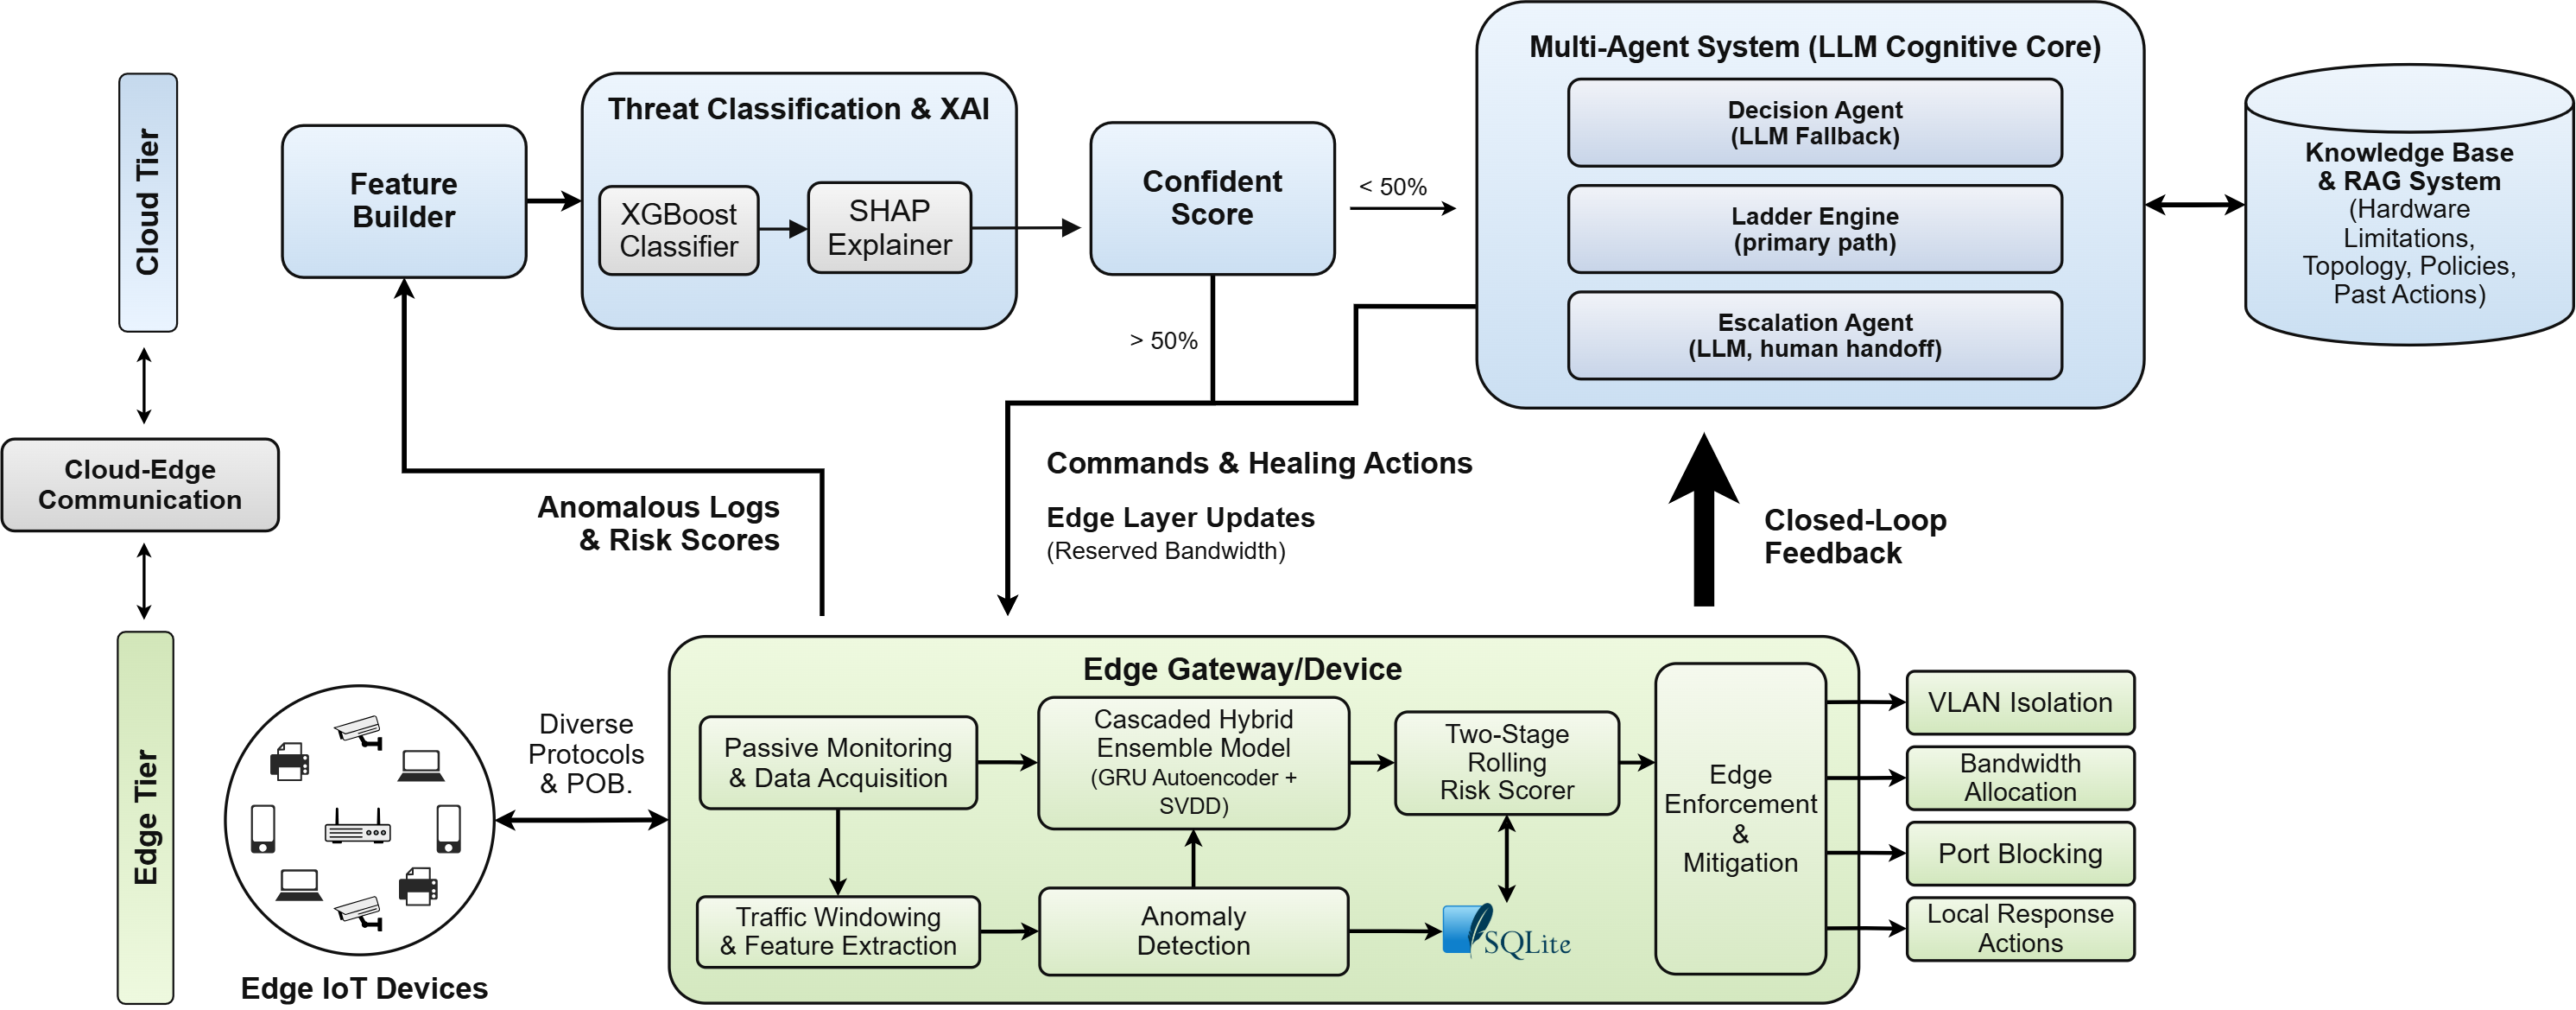
\includegraphics[width=5in]{Images/system_architecture.png}
	\end{center}
	\caption{High-level system architecture. The edge tier runs its own GRU+Deep SVDD anomaly ensemble and rolling risk score entirely locally (dashed box); as discussed in Section \ref{sec:cloud_classification}, this score is not currently transmitted to the cloud, which classifies every raw windowed telemetry submission independently. In the cloud tier, a deterministic Ladder Engine is the primary healing-decision path; the Decision and Escalation Agents are LLM-backed fallbacks consulted only when the ladder cannot resolve an incident on its own (Section \ref{sec:multi_agent}), and the Dashboard Reporting Agent runs in parallel on every classified window.}
	\label{fig:architecture}
\end{figure}

\section{Edge Layer: Traffic Monitoring and Representation}

At the edge layer, passive network monitoring is employed to capture IoT traffic without introducing latency into device operations. As shown in Figure \ref{fig:architecture}, this responsibility is split across two modules within the Edge Gateway/Device: \textbf{Passive Monitoring \& Data Acquisition}, which observes traffic from the attached IoT device population without inserting itself into the data path, and \textbf{Traffic Windowing \& Feature Extraction}, which aggregates the captured traffic into time-based windows and derives the statistical and behavioral descriptors used by the detection ensemble.

Passive monitoring is implemented through observation of traffic that is already traversing the gateway-for example, via port mirroring on a managed switch or a network tap positioned ahead of the gateway's forwarding path-so that the acquisition step itself adds no additional hops, and therefore no additional latency, to the traffic it observes. This is a deliberate design constraint rather than an implementation detail: Chapter \ref{cha:introduction} establishes that the endpoint population this framework protects cannot tolerate an inline security appliance that introduces its own processing delay, since several of the attack patterns motivating this work conclude within seconds to a few minutes, and any latency contributed by the detection pipeline itself would eat directly into an already narrow window for response.

From the raw captured traffic, the Traffic Windowing \& Feature Extraction module aggregates packets into fixed-length time windows per device and computes a fixed set of 36 statistical and behavioral descriptors for each window, listed in full in Table \ref{tb:feature_register}. These fall into two families: five \texttt{log\_*} features summarising the application- or message-layer traffic observed in the window (message counts, inter-message interval statistics, and the range and type diversity of the data values carried), and 31 \texttt{network\_*} features summarising the packet- and connection-layer traffic (header length, IP length and flags, TCP maximum-segment-size, TCP control-flag counts, inter-packet timing, IP time-to-live, and the cardinality of distinct source/destination IP addresses, MAC addresses, ports, and protocols observed). This split reflects the two levels at which the edge gateway can observe a constrained IoT device: what it is saying, at the level of the messages an application-layer protocol exchanges, and how it is saying it, at the level of the underlying packet stream-consistent with the general family of flow-level statistical features used throughout the network-intrusion-detection literature reviewed in Chapter \ref{cha:literature_review}, but fixed here to the specific 36-feature schema the edge-layer models were trained and evaluated against. The resulting per-window feature vector is normalized using a pre-fitted \texttt{MinMaxScaler}, which rescales each feature to the $[0,1]$ range using minimum and maximum values fitted on a benign-traffic calibration set, so that features with different natural scales (e.g., a byte count in the thousands versus a protocol-distribution ratio between 0 and 1) contribute comparably to the downstream model rather than being dominated by whichever feature happens to have the largest raw magnitude. These normalized point features, denoted $x_{scaled}$, serve as one of the two inputs to the anomaly detection ensemble described in Section \ref{sec:hybrid_ensemble}; the other being the sliding window of recent frames consumed by the temporal model.
{\small
\renewcommand{\arraystretch}{1.15}
\begin{longtable}{|>{\centering\arraybackslash}p{0.05\textwidth}|>{\raggedright\arraybackslash}p{0.34\textwidth}|>{\raggedright\arraybackslash}p{0.49\textwidth}|}
\caption{Complete edge-layer feature register: the 36 statistical and behavioral descriptors computed per traffic window and consumed by the GRU + Deep SVDD ensemble.}
\label{tb:feature_register}\\
\hline
\textbf{\#} & \textbf{Feature name} & \textbf{Description} \\
\hline
\endfirsthead
\multicolumn{3}{|c|}{\tablename\ \thetable{} -- continued from previous page}\\
\hline
\textbf{\#} & \textbf{Feature name} & \textbf{Description} \\
\hline
\endhead
\multicolumn{3}{|r|}{\textit{Continued on next page}}\\
\hline
\endfoot
\endlastfoot
0 & \path{log_data-ranges_avg} & Average range spanned by data values carried in the window's application/log-level messages. \\ \hline
1 & \path{log_data-ranges_std_deviation} & Standard deviation of the same data-range measure. \\ \hline
2 & \path{log_data-types} & Diversity of data types observed across the window's log-level messages (small integer-coded categorical). \\ \hline
3 & \path{log_interval-messages} & Inter-message interval statistic at the application/log-message level. \\ \hline
4 & \path{log_messages_count} & Count of application/log-level messages observed in the window. \\ \hline
5 & \path{network_header-length_avg} & Average packet header length. \\ \hline
6 & \path{network_header-length_std_deviation} & Standard deviation of packet header length. \\ \hline
7 & \path{network_interval-packets} & Inter-packet interval statistic. \\ \hline
8 & \path{network_ip-flags_avg} & Average value of the IP header flags field. \\ \hline
9 & \path{network_ip-flags_min} & Minimum value of the IP header flags field. \\ \hline
10 & \path{network_ip-length_avg} & Average IP total-length field value. \\ \hline
11 & \path{network_ip-length_max} & Maximum IP total-length field value. \\ \hline
12 & \path{network_ip-length_min} & Minimum IP total-length field value. \\ \hline
13 & \path{network_ips_all} & Cardinality/encoding of all distinct IP addresses (source and destination) observed. \\ \hline
14 & \path{network_ips_all_count} & Count of distinct IP addresses observed. \\ \hline
15 & \path{network_ips_dst} & Cardinality/encoding of distinct destination IP addresses observed. \\ \hline
16 & \path{network_macs_all} & Cardinality/encoding of distinct MAC addresses observed. \\ \hline
17 & \path{network_mss_avg} & Average TCP Maximum Segment Size. \\ \hline
18 & \path{network_mss_std_deviation} & Standard deviation of TCP Maximum Segment Size. \\ \hline
19 & \path{network_packet-size_avg} & Average packet size. \\ \hline
20 & \path{network_packet-size_min} & Minimum packet size. \\ \hline
21 & \path{network_packets_all_count} & Total packet count in the window. \\ \hline
22 & \path{network_ports_all} & Cardinality/encoding of distinct ports observed. \\ \hline
23 & \path{network_ports_all_count} & Count of distinct ports observed. \\ \hline
24 & \path{network_protocols_all} & Cardinality/encoding of distinct protocols observed. \\ \hline
25 & \path{network_protocols_all_count} & Count of distinct protocols observed. \\ \hline
26 & \path{network_protocols_dst} & Cardinality/encoding of distinct destination-side protocols. \\ \hline
27 & \path{network_protocols_src} & Cardinality/encoding of distinct source-side protocols. \\ \hline
28 & \path{network_tcp-flags-fin_count} & Count of TCP FIN flags observed. \\ \hline
29 & \path{network_tcp-flags-rst_count} & Count of TCP RST flags observed. \\ \hline
30 & \path{network_tcp-flags-syn_count} & Count of TCP SYN flags observed. \\ \hline
31 & \path{network_time-delta_avg} & Average inter-arrival time delta between packets. \\ \hline
32 & \path{network_time-delta_max} & Maximum inter-arrival time delta. \\ \hline
33 & \path{network_time-delta_min} & Minimum inter-arrival time delta. \\ \hline
34 & \path{network_time-delta_std_deviation} & Standard deviation of inter-arrival time delta. \\ \hline
35 & \path{network_ttl_avg} & Average IP time-to-live value. \\ \hline
\end{longtable}
}

\section{Cascaded Hybrid (Stacked) Ensemble Model}\label{sec:hybrid_ensemble}

To robustly identify anomalous behavior without requiring labeled attack data during training, the edge layer deploys a one-class cascaded hybrid ensemble, shown as the \textbf{Cascaded Hybrid Ensemble Model (GRU Autoencoder + Deep SVDD)} block in Figure \ref{fig:architecture}. This architecture pairs a deep temporal model with a deep one-class boundary method, leveraging the strengths of both: the GRU autoencoder captures how a device's traffic evolves over a short recent history, while Deep Support Vector Data Description (Deep SVDD) provides a compact, unsupervised description of what a benign combination of temporal and point-in-time features looks like, against which any new observation can be scored. Figure \ref{fig:hybrid_ensemble} expands this block into its constituent pipeline, showing how the GRU's temporal embedding and the current timestep's scaled point features are concatenated before being scored by the Deep SVDD boundary; the three numbered steps below correspond directly to the stages shown in that diagram.

\begin{enumerate}
	\item \textbf{Temporal Feature Extraction:} A single-layer Gated Recurrent Unit (GRU) autoencoder \cite{Cho2014} with a hidden dimension of 64 processes a sliding window of recent frames (size 8). The GRU is a simplified recurrent architecture that merges the input and forget gates of a Long Short-Term Memory (LSTM) cell into a single update gate and removes the separate cell state, which reduces the number of trainable parameters and the per-step computation relative to an LSTM while retaining the ability to model sequential dependencies in the traffic-the property this project relies on to build a temporal fingerprint of device behavior. The GRU is trained as an autoencoder, i.e., it is optimized to reconstruct its own input window rather than to predict a label, so that its reconstruction error is large precisely when the input window departs from the sequential patterns seen in benign training traffic. The GRU is optimized using the RMSprop algorithm \cite{Tieleman2012} ($\alpha=0.99$, learning rate $0.002$). RMSprop is specifically selected over Adam because its moving average of squared gradients better stabilizes training against the noisy, non-stationary reconstruction loss typical of IoT traffic. The last hidden state of the GRU, $h_n[-1]$, serves as a 64-dimensional temporal embedding representing sequential device behavior.

	\item \textbf{Feature Fusion and One-Class Boundary Estimation:} The temporal embedding is concatenated with the current timestep's MinMax-scaled point features to create a fused feature vector, $v_{fused} = h_n[-1] \oplus x_{scaled}$. This fused vector is the input to a Deep Support Vector Data Description (Deep SVDD) model \cite{Ruff2018}, trained entirely on benign traffic. Deep SVDD extends the classical, kernel-based SVDD of Tax and Duin \cite{Tax2004} by replacing the fixed kernel-induced feature map with a neural network $\phi(\cdot\,; W)$ whose weights $W$ are learned jointly with the one-class objective, rather than fixed in advance or selected from a small family of kernel functions. In the one-class variant used here-appropriate because the training set is (assumed) entirely benign, so no soft boundary or outlier-tolerance slack term is required-the network is trained to map every benign training vector as close as possible to a fixed centre $c$ in the output space:
	\begin{equation}
	\min_{W} \; \frac{1}{n} \sum_{i=1}^{n} \lVert \phi(v_i; W) - c \rVert^2 \; + \; \frac{\lambda}{2} \sum_{l} \lVert W_l \rVert_F^2,
	\label{e:svdd_primal}
	\end{equation}
	where $n$ is the number of benign training vectors, $c$ is fixed in advance (for example, as the mean of an initial forward pass over the training set, following \cite{Ruff2018}) rather than optimised jointly, $\lambda$ is a weight-decay regularisation coefficient applied per layer $l$, and the network $\phi(\cdot\,;W)$ is constructed without bias terms and without bounded activation functions in its final layers, an architectural constraint Ruff et al. show is necessary to prevent the trivial ``hypersphere collapse'' solution in which the network learns to map every input to $c$ regardless of its content \cite{Ruff2018}. Minimising Equation \ref{e:svdd_primal} concentrates the benign training population as tightly as possible around $c$ in the learned output space, so that a genuinely benign vector observed at inference time is expected to land close to $c$, while a vector whose fused temporal-and-point-feature profile differs materially from benign behaviour is expected to land further away. This is the property that makes the resulting distance a usable one-class anomaly score, and is exactly analogous to the volume-minimisation intuition of classical SVDD's hypersphere, but achieved through a learned representation rather than a fixed kernel.

	\item \textbf{Inference:} At runtime, a new fused feature vector $v$ is scored by its squared distance from the learned centre,
	\begin{equation}
	d(v) = \lVert \phi(v; W) - c \rVert^2,
	\label{e:svdd_score}
	\end{equation}
	which is small when $v$ resembles the benign training population and large when it does not. This continuous distance score $d(v)$ is compared against an optimal threshold (determined offline via the F1 precision-recall curve on a validation set) to flag the time window as anomalous, corresponding to the \textbf{Anomaly Detection} step in Figure \ref{fig:architecture}.
\end{enumerate}

Deep SVDD is preferred over a purely distance-based or density-based one-class method for this fused vector for two reasons specific to this design. First, because $v_{fused}$ concatenates a 64-dimensional learned temporal embedding with a smaller set of point features, the two halves of the vector have different statistical structure, and a jointly learned neural boundary can adapt to this combined space more flexibly than a boundary defined directly in terms of Euclidean distance to training examples, or than a fixed kernel selected without reference to the specific structure of a GRU-produced embedding. Second, Deep SVDD's boundary is defined purely from benign data and does not require an attack-labeled dataset during training, which matches the practical constraint-already discussed in Chapter \ref{cha:literature_review}-that verified attack traffic for a given IoT deployment is typically far scarcer than benign traffic, and often unavailable altogether prior to deployment. Chapter \ref{cha:results} reports that, on the evaluation data available for this project, a standalone Deep SVDD model performs considerably worse than the fused GRU + Deep SVDD ensemble, which is the empirical justification, alongside the architectural reasoning above, for pairing it with the GRU's temporal embedding rather than deploying it directly on point features alone.

\begin{figure}[htbp]
	\begin{center}
	\resizebox{5in}{!}{%
	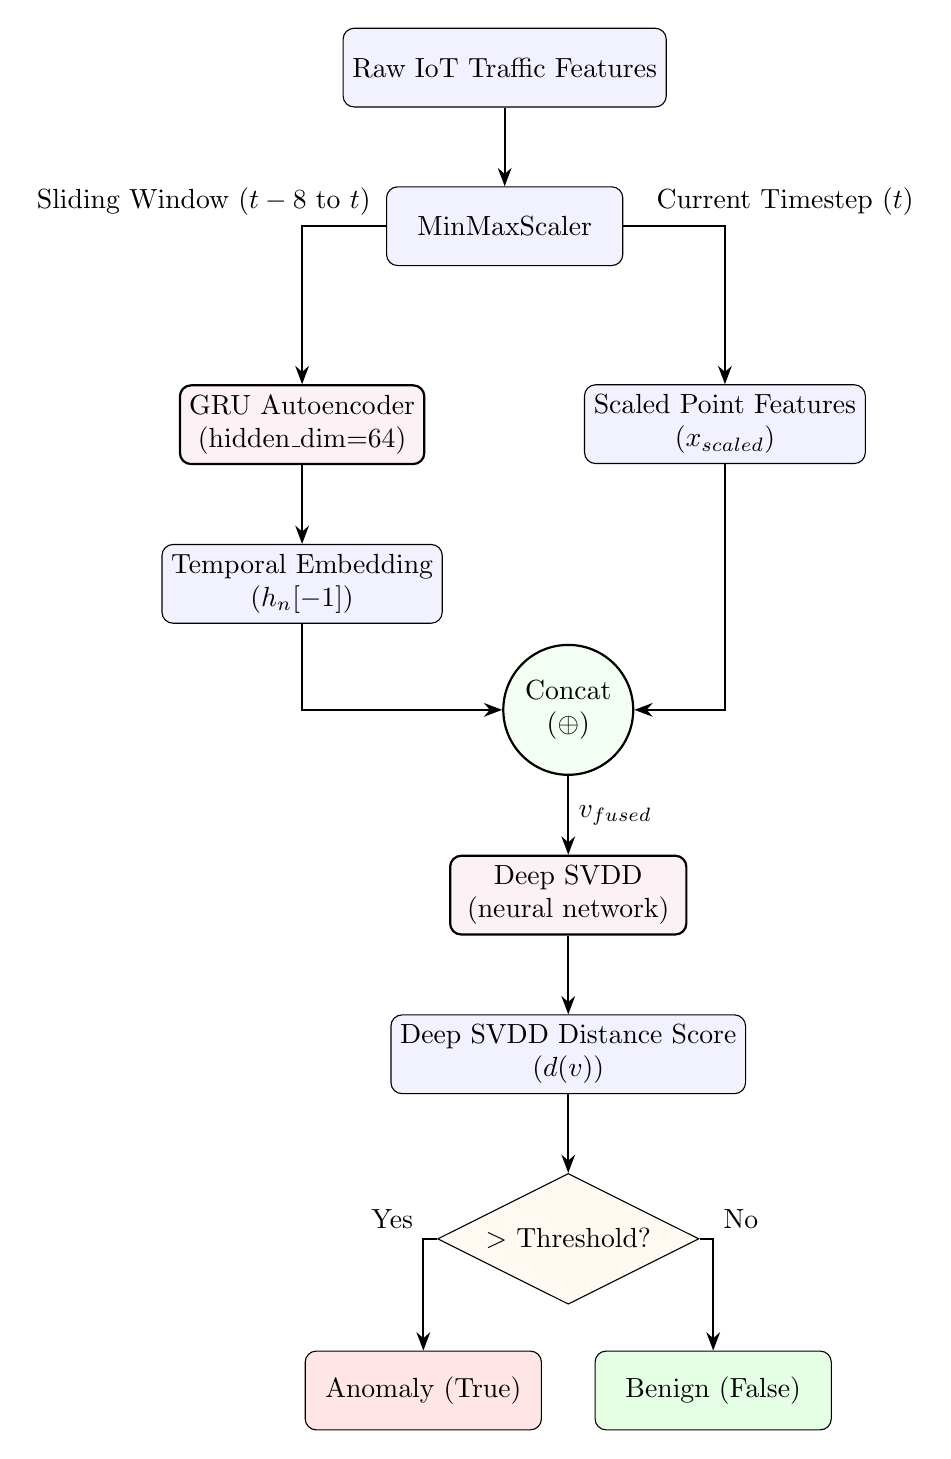
\begin{tikzpicture}[
		>=Stealth,
		node distance=1.5cm and 2cm,
		box/.style={draw, rectangle, rounded corners, minimum width=3cm, minimum height=1cm, align=center, fill=blue!5},
		model/.style={draw, rectangle, rounded corners, minimum width=3cm, minimum height=1cm, align=center, fill=purple!5, thick},
		fusion/.style={draw, circle, minimum size=1.5cm, align=center, fill=green!5, thick},
		decision/.style={draw, diamond, aspect=2, minimum width=2.5cm, minimum height=1cm, align=center, fill=orange!5}
	]

	% Nodes
	\node[box] (input) {Raw IoT Traffic Features};
	\node[box, below=1cm of input] (scaler) {MinMaxScaler};

	\node[model, below left=1.5cm and -0.5cm of scaler] (gru) {GRU Autoencoder \\ (hidden\_dim=64)};
	\node[box, below=1cm of gru] (embedding) {Temporal Embedding \\ ($h_n[-1]$)};

	\node[box, below right=1.5cm and -0.5cm of scaler] (point) {Scaled Point Features \\ ($x_{scaled}$)};

	\node[fusion, below right=0.5cm and 1cm of embedding] (concat) {Concat \\ ($\oplus$)};

	\node[model, below=1cm of concat] (svdd) {Deep SVDD \\ (neural network)};
	\node[box, below=1cm of svdd] (score) {Deep SVDD Distance Score \\ ($d(v)$)};

	\node[decision, below=1cm of score] (threshold) {$>$ Threshold?};

	\node[box, fill=red!10, below left=1cm and -0.5cm of threshold] (anomaly) {Anomaly (True)};
	\node[box, fill=green!10, below right=1cm and -0.5cm of threshold] (benign) {Benign (False)};

	% Arrows
	\draw[->, thick] (input) -- (scaler);

	\draw[->, thick] (scaler) -| node[above left, xshift=1cm] {Sliding Window ($t-8$ to $t$)} (gru);
	\draw[->, thick] (scaler) -| node[above right, xshift=-1cm] {Current Timestep ($t$)} (point);

	\draw[->, thick] (gru) -- (embedding);

	\draw[->, thick] (embedding) |- (concat);
	\draw[->, thick] (point) |- (concat);

	\draw[->, thick] (concat) -- node[right] {$v_{fused}$} (svdd);
	\draw[->, thick] (svdd) -- (score);
	\draw[->, thick] (score) -- (threshold);

	\draw[->, thick] (threshold) -| node[above left] {Yes} (anomaly);
	\draw[->, thick] (threshold) -| node[above right] {No} (benign);

	\end{tikzpicture}%
	}
	\end{center}
	\caption{Block diagram of the cascaded hybrid ensemble showing the GRU pipeline and feature concatenation with the Deep SVDD one-class boundary.}
	\label{fig:hybrid_ensemble}
\end{figure}

\FloatBarrier
\section{Two-Stage Rolling Risk Scoring Mechanism}

Instead of triggering alerts on isolated anomalies, the edge system calculates a persistent per-device risk score, $R \in [0,1]$, to identify sustained malicious activity. This is the mechanism shown as the \textbf{Two-Stage Rolling Risk Scorer} in Figure \ref{fig:architecture}, positioned between the ensemble model and the Edge Enforcement \& Mitigation module.

\textbf{Stage 1: Ensemble Scoring.} While the Deep SVDD boundary's binary decision (Equation \ref{e:svdd_score} compared against the fitted threshold) controls the discrete anomaly flag logged at the \textbf{Anomaly Detection} step, a combined continuous score is also generated for every window of telemetry, so that the risk scorer has graded evidence to work with rather than a single bit per window. Both the GRU reconstruction Mean Squared Error (MSE) and the Deep SVDD distance score $d(v)$ are independently normalized to $[0,1]$ using the same offline-fitted scaling bounds used elsewhere in the pipeline, yielding $S_{gru}$ and $S_{svdd}$ respectively.

\textbf{Stage 2: Rolling Risk Scorer.} The risk score $R$ is dynamically updated per window based on a weighted accumulation and decay mechanism. If a window is flagged as anomalous, the score is increased by a delta, $\Delta R$, defined as:
\begin{equation}
\Delta R = \frac{1}{2} \left( W_{hit} + W_{gru} \cdot S_{gru} + W_{svdd} \cdot S_{svdd} + B_{repeat} \right)
\label{e:delta_r}
\end{equation}
where $W_{hit} = 0.35$ is a fixed penalty applied to every flagged window regardless of its score, $W_{gru} = 0.45$ weights the GRU's continuous reconstruction-error contribution, and $W_{svdd} = 0.40$ weights the Deep SVDD boundary's continuous distance-score contribution. The term $B_{repeat}$ is a repeat-offender boost (up to $0.20$), scaled by the number of consecutive anomalous windows (capped at 5), so that a device flagged repeatedly in immediate succession accumulates risk faster than one flagged once and then not again. The new risk score is clamped at a maximum of $1.0$:
\begin{equation}
R_{t} = \min(R_{t-1} + \Delta R, 1.0)
\label{e:risk_increase}
\end{equation}

Conversely, if the window is benign, the consecutive anomaly counter resets, and the score decays by a fixed penalty, bottoming out at a baseline default of $0.05$ (rather than $0$, so that a device with any recent history of suspicion does not require a full re-accumulation from a completely clean state after a single benign window):
\begin{equation}
R_{t} = \max(R_{t-1} - 0.04, 0.05)
\label{e:risk_decay}
\end{equation}

To illustrate how Equations \ref{e:delta_r}--\ref{e:risk_decay} behave in practice, consider a device at baseline risk $R_{t-1} = 0.05$ that is flagged anomalous with a moderately strong GRU reconstruction error ($S_{gru} = 0.6$) and a moderately strong Deep SVDD distance score ($S_{svdd} = 0.5$), on the first anomalous window in a sequence (so $B_{repeat} = 0$, since the boost only accrues on \emph{consecutive} anomalous windows beyond the first). Equation \ref{e:delta_r} gives $\Delta R = \frac{1}{2}(0.35 + 0.45 \times 0.6 + 0.40 \times 0.5 + 0) = \frac{1}{2}(0.35 + 0.27 + 0.20) = 0.41$, so, applying the clamped update of Equation \ref{e:risk_increase}, the risk score rises to $R_t = \min(0.05 + 0.41, 1.0) = 0.46$ after a single flagged window. If the same device is flagged on four further consecutive windows with similar scores, the repeat-offender boost climbs toward its cap of $0.20$ over those windows, pushing $\Delta R$ higher each time and driving $R$ toward the $1.0$ ceiling well before the fifth consecutive hit-consistent with the design intent that a short burst of repeated, consistent anomalies should escalate quickly. By contrast, a single flagged window followed immediately by benign traffic decays by only $0.04$ per benign window (Equation \ref{e:risk_decay}), meaning that an isolated anomalous window elevates $R$ substantially more than a single benign window brings it back down; the risk score is deliberately asymmetric, rising faster than it falls, so that a device's history of suspicion persists for several benign windows rather than being erased by the very next one.

This persistent state is stored in a local SQLite database, ensuring risk profiles survive edge node reboots. As Figure \ref{fig:architecture} shows, this database serves two related but distinct roles: it is the destination of the discrete anomaly flags produced at the \textbf{Anomaly Detection} step (the historical log of which windows were flagged and why), and it is the persistent store that the \textbf{Two-Stage Rolling Risk Scorer} itself reads from and writes to on every update, so that the current value of $R$ for every device under a gateway's supervision is durable across process restarts and power-cycle events rather than held only in volatile memory.

\textbf{Scope of the risk score in the current implementation.} The mechanism described above is the edge tier's local detection and evidence-accumulation logic, and it is exercised and validated entirely on the edge side. In the cloud-layer implementation described in the remainder of this chapter, the risk score $R$ is not itself transmitted to, or consumed by, the cloud tier: the cloud classifies every incoming window independently (Section \ref{sec:cloud_classification}), and an earlier design that streamed the edge's computed risk score and anomaly flag to the cloud as a separate channel was removed during development in favour of classifying directly off the raw windowed telemetry. The two tiers are consequently coupled only through the raw-telemetry and healing-command channels described in the remainder of this chapter, not through $R$ itself; Section \ref{sec:limitations_integration} in Chapter \ref{cha:results} discusses the further, more basic integration gap this creates between the two layers' current transport implementations.

\begin{figure}[t!]
	\begin{center}
		\IfFileExists{Images/correlation_heatmap.png}
			{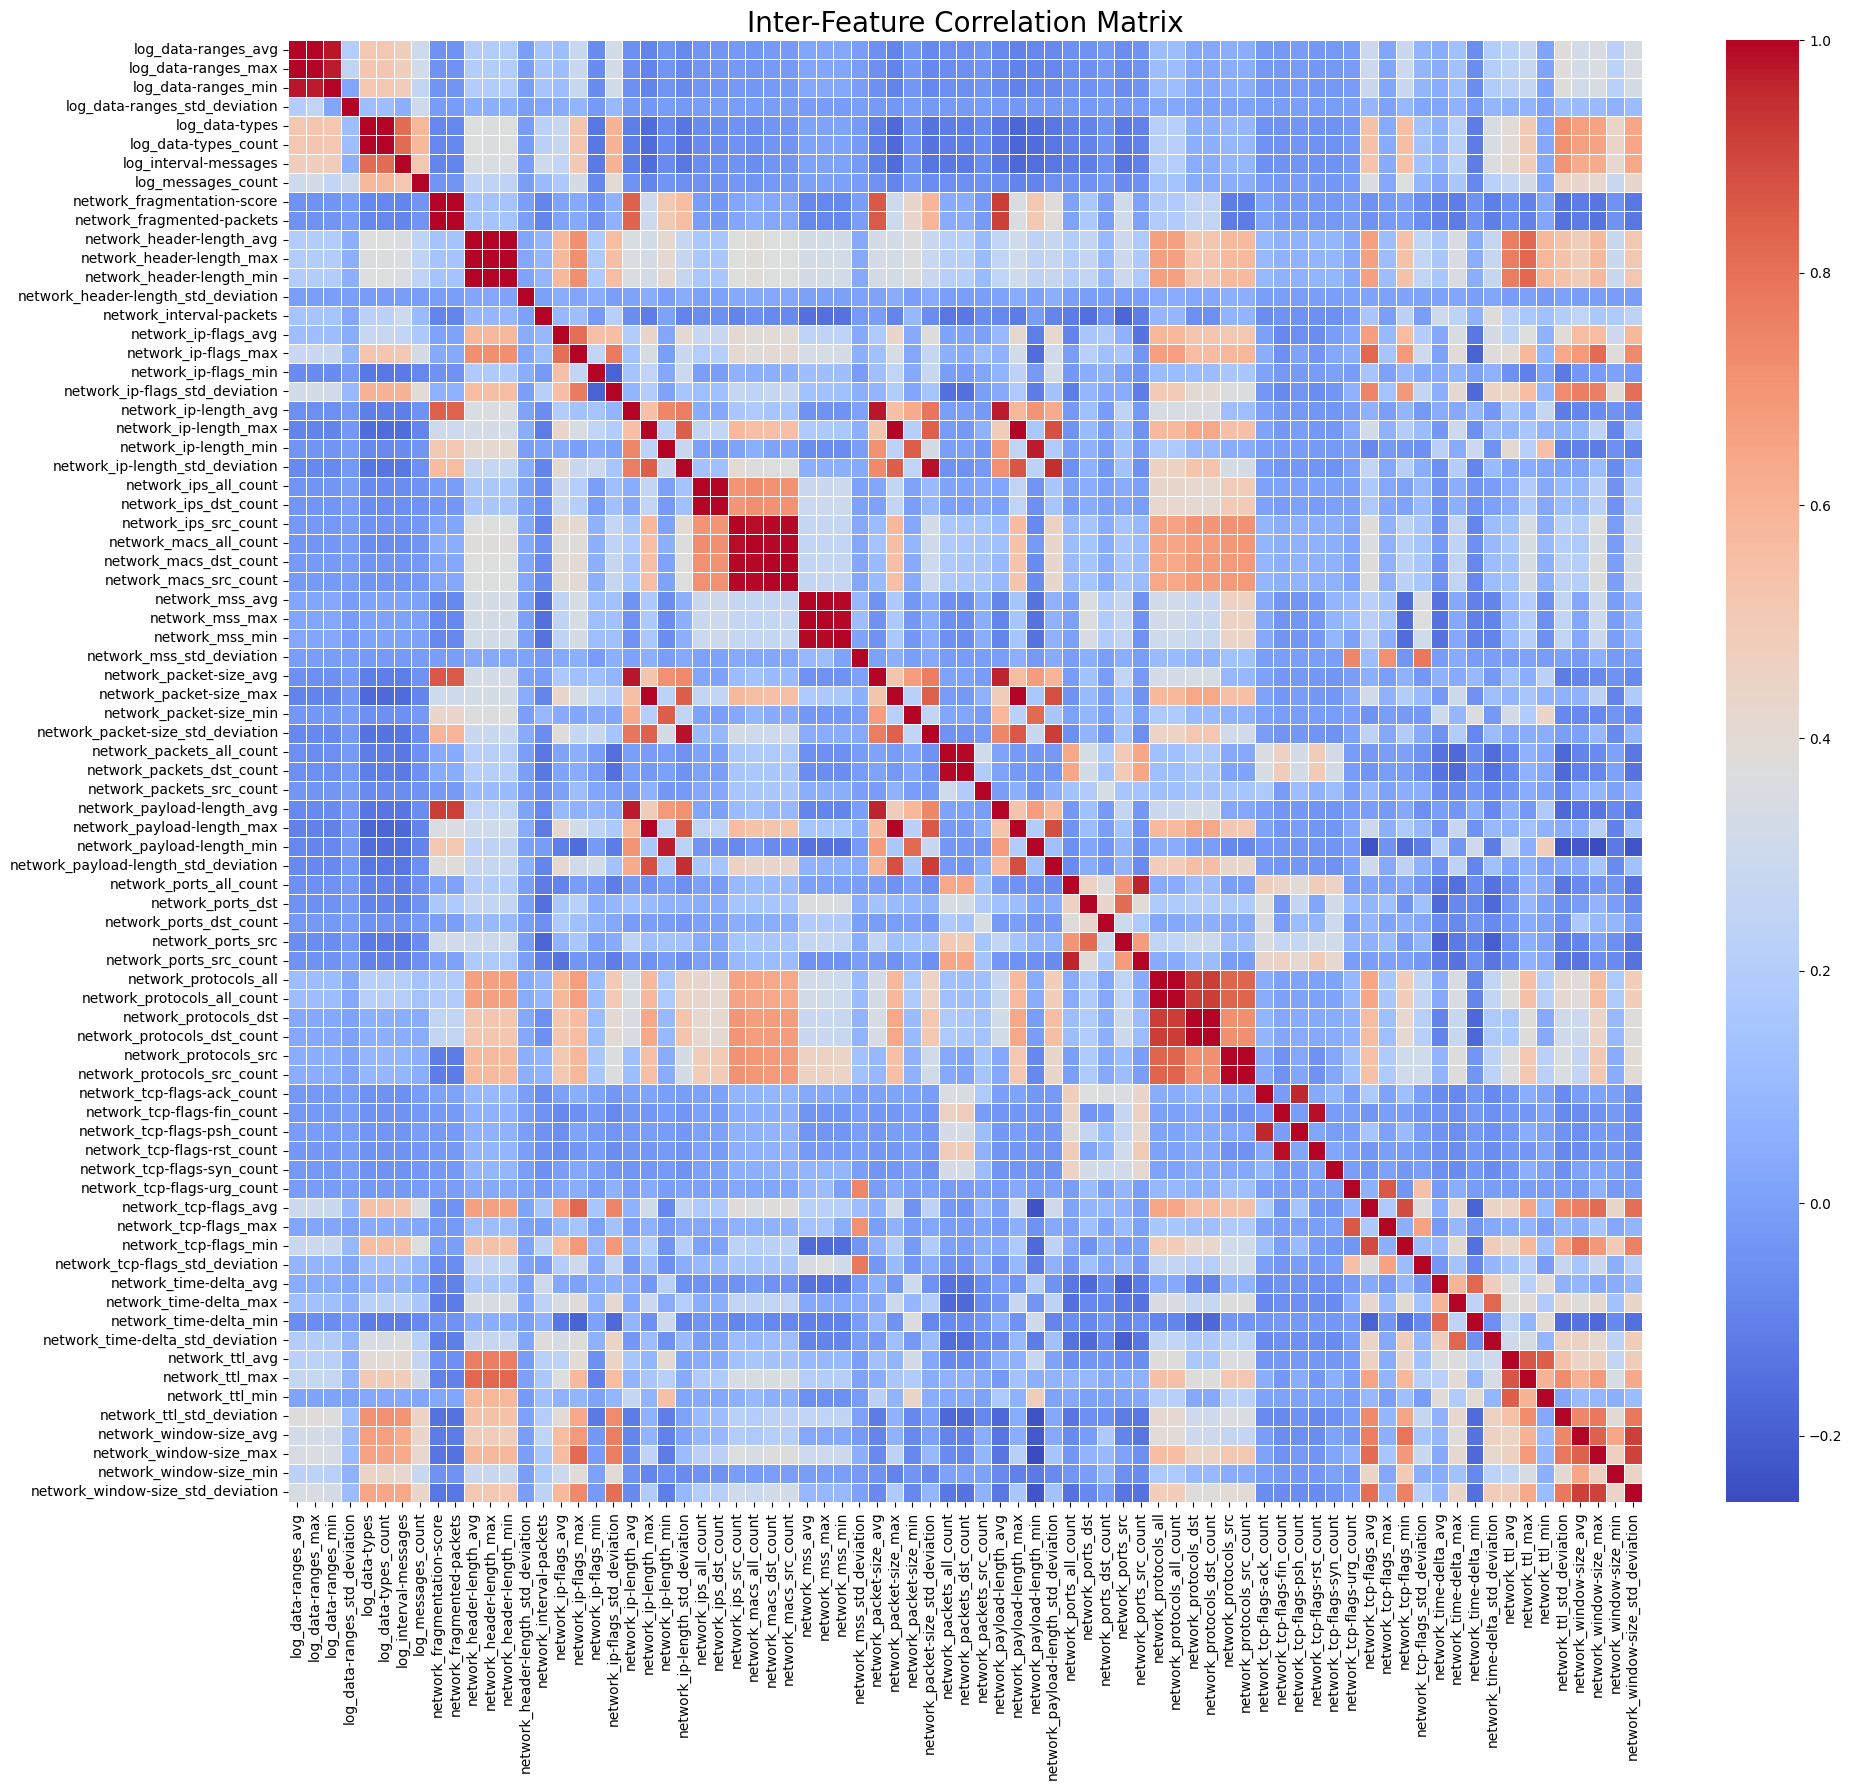
\includegraphics[width=5in]{Images/correlation_heatmap.png}}
			{\rule{5in}{4in} % Placeholder -- add file at Images/correlation_heatmap.png
			\\[-4.2cm]\centering\textit{\small [Image not yet added: Images/correlation\_heatmap.png]}\\[4in]}
	\end{center}
	\caption{Pairwise correlation heatmap of the 81-feature dataset used to identify the 25 features removed in Step 3 of the preprocessing pipeline (correlation $>0.95$ with another retained feature).}
	\label{fig:correlation_heatmap}
\end{figure}

\FloatBarrier
\section{Cloud Layer: Threat Classification and XAI}\label{sec:cloud_classification}

The edge gateway forwards every completed traffic window to the cloud tier over the \textbf{Cloud-Edge Communication} channel shown in Figure \ref{fig:architecture}, via a single HTTP ingestion endpoint that accepts the window's raw, per-connection records (device identifier, window start/end timestamps, and the list of individual connection-log entries observed in that window) rather than a pre-computed feature vector or risk score. This channel is deliberately bidirectional and is drawn as a distinct component in the architecture rather than folded into either tier, because it carries two structurally different kinds of traffic that must both be accommodated without contending with the gateway's normal operational load: raw windowed telemetry flows upward from the edge gateway to the cloud tier's classification pipeline, while \textit{Commands \& Healing Actions} flow downward from the healing-decision pipeline back to the edge gateway. As noted in Section \ref{sec:hybrid_ensemble}, this upward flow is independent of the edge's own risk score; the cloud performs its own classification on every window it receives.

\textbf{Feature construction.} A feature-builder module converts the list of raw connection records in a window into a fixed-length numeric vector matching the schema the classifier was trained on. This schema was derived offline through a four-stage preprocessing pipeline applied to the CIC IIoT 2025 dataset (also released as DataSense), a real-time sensor-and-network-traffic benchmark developed by the Canadian Institute for Cybersecurity from a 40-device industrial testbed spanning more than 15 sensor types, released in December 2024 \cite{Firouzi2025}. The dataset's native representation begins at 94 columns per two-second aggregation window (47 numerical, 24 count-based, and 23 object-type or identifier columns); Step 1 removes device-specific identifiers and overlapping multi-level label columns (94 $\to$ 88 features); Step 2 removes raw address-list object-type columns (full IP- and MAC-address lists) that are unique to the collection testbed and would otherwise let a classifier memorise specific devices rather than learn transferable attack patterns, retaining only their associated count-based features (88 $\to$ 81); Step 3 removes 25 features found to be pairwise-correlated above 0.95 with another retained feature (81 $\to$ 53), eliminating redundant signal rather than distinct information (Figure \ref{fig:correlation_heatmap}); and Step 4 fits an XGBoost classifier on the resulting 53-feature, 112{,}117-record cleaned dataset and retains only the top 30 features by gain-based importance, a 43\% reduction from 53 (Figure \ref{fig:feature_importance})-this final 30-feature set is the schema the deployed classifier described in this section expects. Because the edge layer forwards connection-log-style aggregates-per-connection byte and packet counts, connection state, ports, protocol-rather than true packet-level captures, only a subset of this 30-feature schema can be populated from genuinely observed data at inference time; features that depend on packet-level signals unavailable at this granularity (for example, IP time-to-live statistics, TCP window size, and maximum-segment-size) are populated with a fixed placeholder value rather than left undefined, so that the vector remains well-formed but is not fully informative on every dimension. This gap between the granularity the classifier was trained on and the granularity the edge layer can practically supply is, as discussed in Chapter \ref{cha:results}, the single most consequential limitation identified when this pipeline was evaluated end-to-end.

\begin{figure}[htbp]
	\begin{center}
		\IfFileExists{Images/feature_importance.png}
			{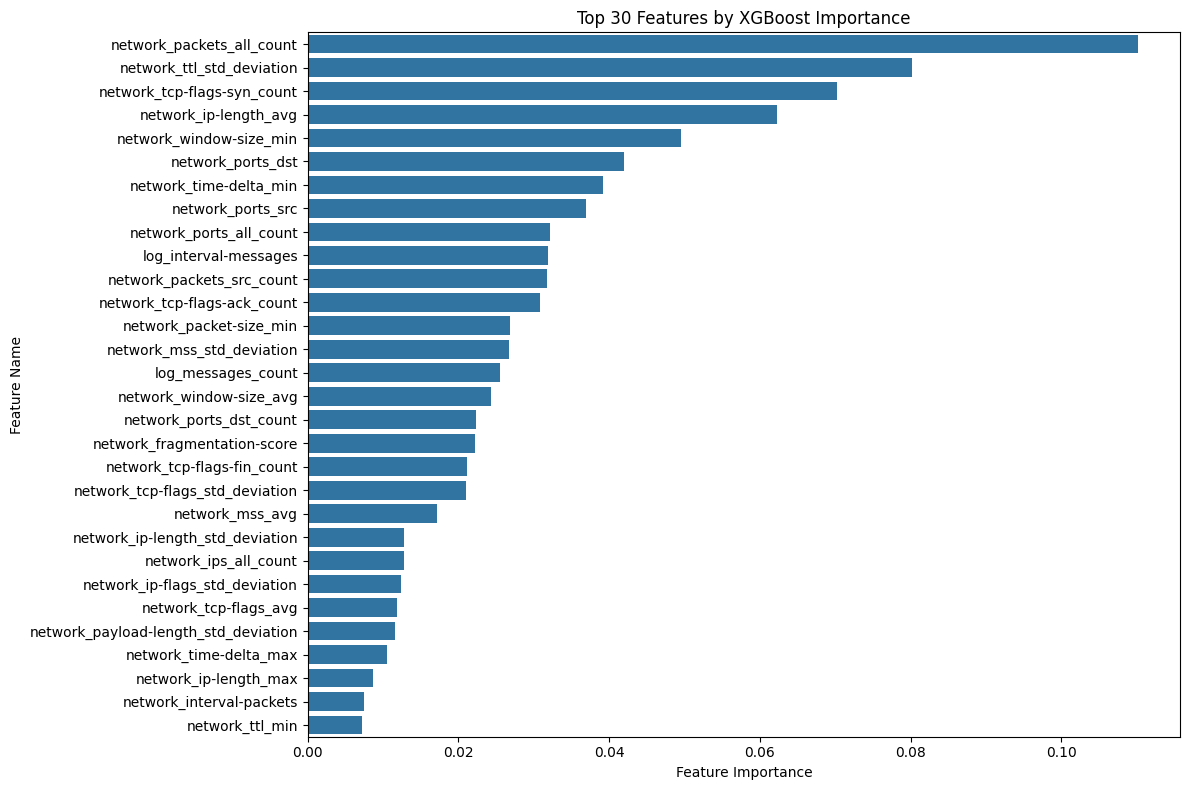
\includegraphics[width=5in]{Images/feature_importance.png}}
			{\rule{5in}{4in} % Placeholder -- add file at Images/feature_importance.png
			\\[-4.2cm]\centering\textit{\small [Image not yet added: Images/feature\_importance.png]}\\[4in]}
	\end{center}
	\caption{Gain-based feature importance ranking from the XGBoost model fitted in Step 4 of the preprocessing pipeline, used to select the top 30 of the remaining 53 features.}
	\label{fig:feature_importance}
\end{figure}

\textbf{Classification.} In the cloud, a pre-trained XGBoost classifier categorizes the specific attack type from the constructed feature vector. XGBoost \cite{ChenGuestrin2016} is a gradient-boosted decision-tree ensemble that builds an additive sequence of shallow regression trees $\hat{y} = \sum_{k=1}^{K} f_k(x)$, where each tree $f_k$ is fitted to reduce the residual error left by the trees before it, subject to an explicit regularization penalty on tree complexity that discourages overfitting to any single training batch of attack traffic. It is selected for this stage over a comparable neural classifier because, on the tabular, engineered flow-features produced by the edge layer's windowing step, tree-boosting ensembles of this kind have consistently matched or exceeded deep-learning classifiers in both accuracy and inference speed on network-flow benchmarks, as discussed in the literature reviewed in Chapter \ref{cha:literature_review}, while remaining directly compatible with the feature-attribution method described next.

The classifier is trained against a fine-grained label set considerably larger than the set of remediation playbooks documented in Appendix \ref{app:healing_actions}: dozens of specific attack sub-types (for example, distinct fine-grained labels for different DDoS flood variants, or for SSH- versus Telnet-targeted brute-force) rather than one label per attack class. Rather than requiring a separate healing playbook for every fine-grained label, the classifier's predicted class probabilities are summed into a small number of \textit{grouped buckets}-\texttt{benign}, \texttt{ddos}, \texttt{port\_scan}, \texttt{bruteforce}, \texttt{mirai\_botnet}, \texttt{lateral\_movement}, \texttt{exfiltration}, and a catch-all \texttt{unhandled\_attack} bucket for fine-grained labels (such as man-in-the-middle and web-application labels) that do not map onto any of the other seven-and the winning bucket's summed probability becomes the reported classification confidence. Both the fine-grained label and the grouped bucket are retained: the grouped bucket is what the healing ladder in Section \ref{sec:multi_agent} keys its playbook selection on, while the fine-grained label is what the SHAP explainer below explains against and what appears in every downstream forensic report. Two of the eight grouped buckets, \texttt{lateral\_movement} and \texttt{exfiltration}, are configured with their own healing playbooks in Appendix \ref{app:healing_actions} but, as verified during evaluation (Chapter \ref{cha:results}), are not currently reachable in practice: no fine-grained label the classifier can output maps onto either bucket, so these two playbooks exist as configured policy without a corresponding trigger path. The training data underlying the feature schema described above (Section \ref{sec:hybrid_ensemble}) itself documents 50 distinct attack types across seven categories-DDoS, DoS, Reconnaissance, Web, Bruteforce, MITM, and Malware/Mirai \cite{Firouzi2025}-and neither \texttt{lateral\_movement} nor \texttt{exfiltration} corresponds to a category in that taxonomy, which is consistent with, and a plausible explanation for, why the classifier has no path to either bucket. The deployed classifier's 76-label fine-grained set does not map one-to-one onto this 50-type source taxonomy, and confirming the exact relationship between the two-whether the production label set extends this dataset's categories with additional sub-types, or was assembled from a broader combination of sources-is noted as a further open item alongside the other integration gaps discussed in Section \ref{sec:limitations_integration}.

A classification is only acted upon by the healing pipeline once its confidence exceeds a fixed gate; classifications below the gate do not open an incident on their own, but are tracked as a rolling low-confidence signal for the same device and attack-type pairing, as described in Section \ref{sec:multi_agent}.

\textbf{Explainability.} Crucially, the classification is passed through a SHAP explainer, computed against the predicted \textit{fine-grained} label rather than the grouped bucket, so that the explanation reflects exactly which sub-type of attack the model believes it has seen. SHapley Additive exPlanations (SHAP), introduced by Lundberg and Lee \cite{Lundberg2017}, assigns each input feature $i$ a contribution value
\begin{equation}
\phi_i = \sum_{S \subseteq F \setminus \{i\}} \frac{|S|!\,(|F|-|S|-1)!}{|F|!} \Big[ f(S \cup \{i\}) - f(S) \Big],
\label{e:shap}
\end{equation}
where $F$ is the full set of input features, $S$ ranges over every subset of the other features, and $f(S)$ is the classifier's expected output when only the features in $S$ are known. Equation \ref{e:shap} is the Shapley value from cooperative game theory, applied here by treating each network feature as a ``player'' contributing to the classifier's output; it has the property that the contributions $\phi_i$ sum exactly to the difference between the model's prediction for a given window and its average prediction, so the attribution is additive and exact rather than a heuristic approximation. Only the top-3 contributing features by $|\phi_i|$ are retained, each tagged with the direction of its contribution, and translated from raw feature codes into short plain-English statements before being passed downstream (for example, describing a high count of unanswered SYN packets as evidence pushing the classification toward a particular attack class). Instead of presenting this XAI output solely to human administrators, the translated SHAP attributions and classification labels are serialized and fed directly into the cognitive healing pipeline described next.

\textbf{Attribution faithfulness.} Because the downstream healing pipeline consumes SHAP attributions directly rather than as an advisory overlay, the attributions themselves must be verified to reflect features the classifier actually relies on rather than plausible-looking but incidental ones. This is quantified with the standard \textit{correctness deletion curve}: features are removed in descending order of $|\phi_i|$ and, at each step, the classifier's average probability assigned to the originally predicted (true) class is measured on the remaining perturbed vector, tracing how quickly the model's confidence collapses as its own top-attributed features are withdrawn. Figure \ref{fig:correctness_deletion} shows the resulting curve on the held-out evaluation set: the true-class probability falls from 0.89 with all features present to 0.50 after removing only the top $\sim$3\% of features, and to 0.22 after removing the top $\sim$7\%, before flattening near the class-prior baseline once roughly 40\% of features have been withdrawn. The area under this perturbation curve (AUPC) is 0.1264, and the sharp, front-loaded drop directly supports the interpretation that the features SHAP surfaces are the ones the classifier is genuinely acting on; the top-3 statements passed to the healing pipeline can therefore be treated as decision-driving evidence rather than post-hoc rationalisation.

\begin{figure}[htbp]
	\begin{center}
		\IfFileExists{Images/correctness_deletion_curve.jpeg}
			{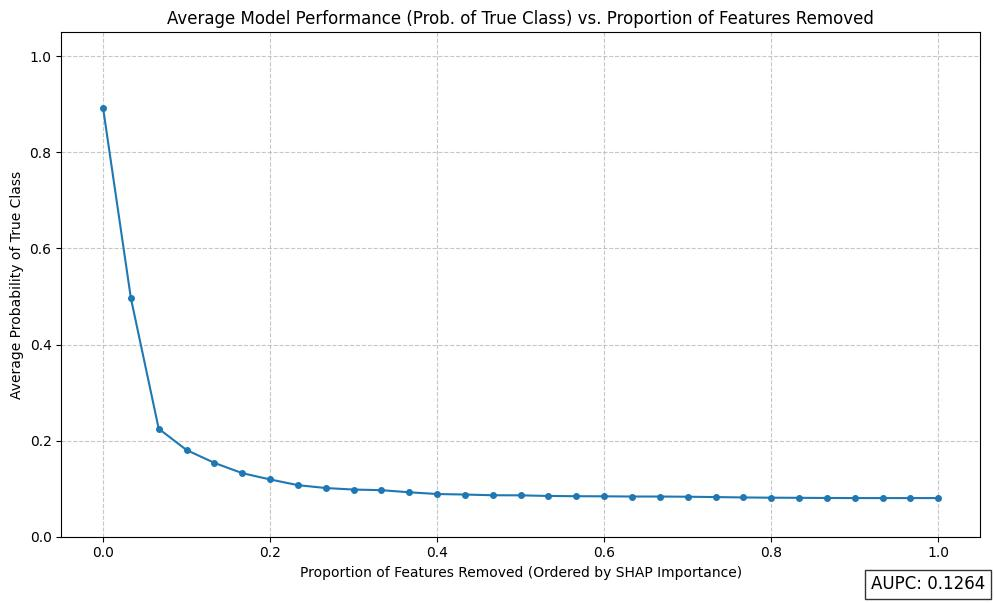
\includegraphics[width=5in]{Images/correctness_deletion_curve.jpeg}}
			{\rule{5in}{3in} % Placeholder -- add file at Images/correctness_deletion_curve.jpeg
			\\[-3.2cm]\centering\textit{\small [Image not yet added: Images/correctness\_deletion\_curve.jpeg]}\\[3in]}
	\end{center}
	\caption{Correctness deletion curve for the SHAP attributions produced by the cloud-tier XGBoost classifier: average probability of the originally predicted (true) class as a growing proportion of features, ordered by descending SHAP importance, is withheld from the input. The steep front-loaded drop (AUPC = 0.1264) indicates that the top-attributed features are the ones the classifier is genuinely acting on.}
	\label{fig:correctness_deletion}
\end{figure}

\FloatBarrier

\section{Multi-Agent System and Self-Healing Orchestration}\label{sec:multi_agent}

Unlike an architecture in which every classified window is handed to a language model to decide a response, the cognitive core of this framework treats the language model as a \textit{fallback} mechanism rather than the default decision-maker. The primary healing decision is made by a deterministic \textbf{ladder engine} operating over the prioritised playbooks documented in Appendix \ref{app:healing_actions}; a language-model agent is only consulted when that deterministic mechanism cannot make a confident decision on its own. This design choice follows directly from the explainability argument developed in Chapter \ref{cha:literature_review}: a playbook whose escalation order is fixed in advance and auditable in a table is inherently more inspectable, before the fact, than a decision an LLM generates fresh each time, so the deterministic path is preferred whenever it is applicable and the language model is reserved for the cases the playbook genuinely cannot cover.

Three distinct roles are served by language-model agents in this design, rather than a single sequential pipeline:

\begin{enumerate}
	\item \textbf{Dashboard Reporting Agent:} Runs on every classification the cloud tier produces, independently of and in parallel with the healing decision described below-a report is generated whether or not any healing action is taken, so that an operator watching the dashboard has visibility into benign and sub-threshold windows as well as acted-upon incidents. It synthesizes the classification, the translated SHAP attributions, and the raw window's descriptive statistics into a structured, human-readable security report (a summary, a severity rating, and a set of indicators), either through a language-model call or, in constrained deployments, a deterministic template.
	\item \textbf{Decision Agent (LLM Fallback):} Consulted only in two specific circumstances the ladder engine cannot resolve on its own: a classification whose confidence stays below the confidence gate on repeated occasions for the same device and attack-type pairing (a persistent low-confidence streak, rather than a single uncertain window), or a classification that lands in the \texttt{unhandled\_attack} bucket, for which no ladder is configured at all (Section \ref{sec:cloud_classification}). In either case, the Decision Agent is grounded by the same Retrieval-Augmented Generation (RAG) mechanism described below and chooses a single action from the healing catalogue, rather than free-composing an arbitrary command.
	\item \textbf{Escalation Agent (Human-Handoff Reporting):} Consulted only once an incident reaches the final tier of its playbook without the device's risk resolving, or once a Decision Agent-selected action itself proves ineffective. Rather than choosing a further automated action, this agent's sole output is a structured operator brief-a plain-language account of the incident timeline and everything already attempted-attached to the incident at the moment it is handed to a human, matching the escalation behaviour already described qualitatively in Chapter \ref{cha:introduction}.
\end{enumerate}

The RAG mechanism that grounds the Decision and Escalation Agents follows the general retrieval-augmented generation pattern introduced by Lewis et al. \cite{Lewis2020}: the markdown-formatted playbooks of Appendix \ref{app:healing_actions}, together with hardware, topology, and policy documents describing the specific edge deployment, are embedded into a vector representation and indexed in advance, and at query time an agent's request (informed by the classification and the translated SHAP attributions) is embedded in the same space and matched against the index to retrieve only the passages most relevant to the device and incident at hand. This retrieved context is then inserted into the prompt given to the language model, so that its output is conditioned on verified, deployment-specific facts-for instance, which VLANs actually exist on the affected switch-rather than on statistically plausible but potentially incorrect assumptions about the network's configuration. A successful Decision Agent action is, in turn, written back into this same retrieval corpus once its effectiveness is confirmed (see \textit{Healing Actions and Closed-Loop Feedback} below), so that the knowledge base a future incident is grounded against includes not only the static playbooks but a growing record of what has actually worked.

\begin{figure}[htbp]
	\begin{center}
	\resizebox{5.5in}{!}{%
	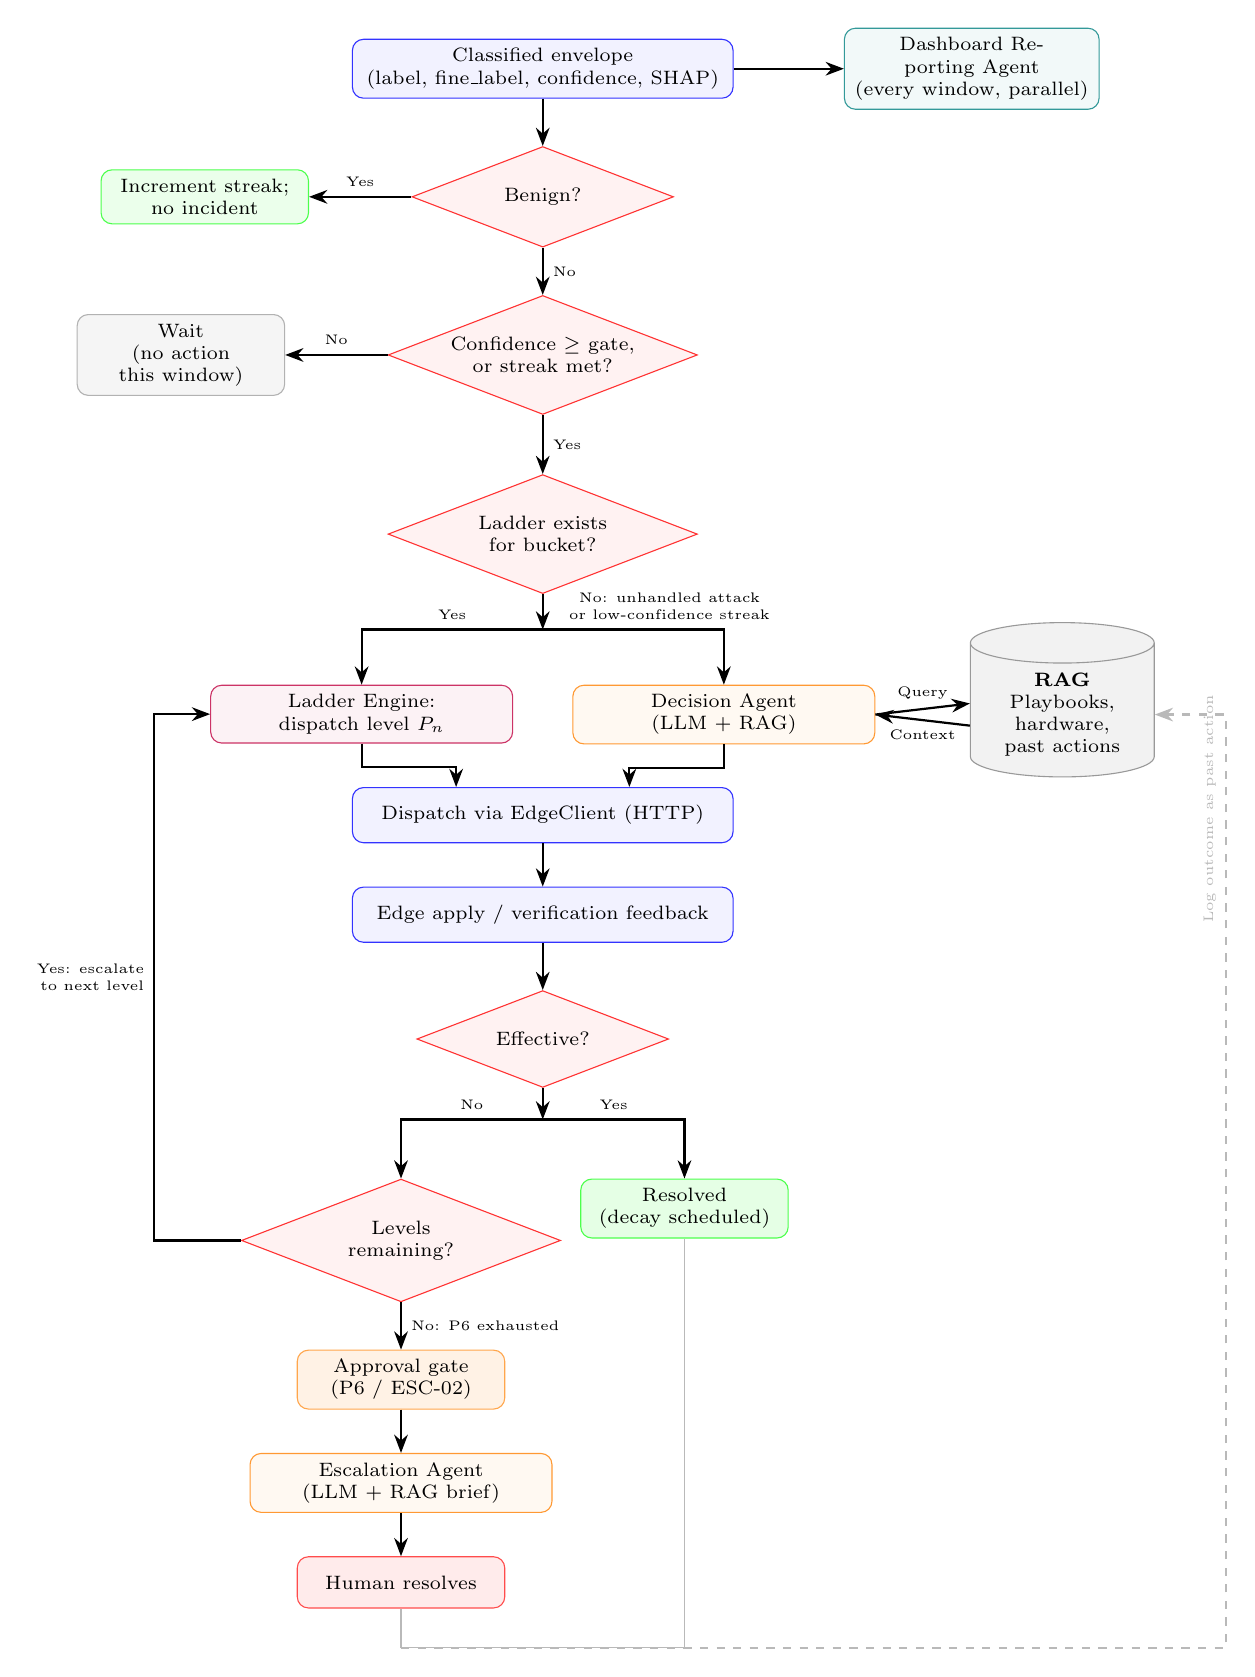
\begin{tikzpicture}[
		>=Stealth,
		node distance=0.65cm,
		data/.style={draw=blue!80, fill=blue!5, rectangle, rounded corners, minimum height=0.7cm, text centered, text width=4.6cm, font=\scriptsize},
		report/.style={draw=teal!80, fill=teal!5, rectangle, rounded corners, minimum height=0.7cm, text centered, text width=3.0cm, font=\scriptsize},
		ladder/.style={draw=purple!80, fill=purple!5, rectangle, rounded corners, minimum height=0.7cm, text centered, text width=3.6cm, font=\scriptsize},
		agent/.style={draw=orange!80, fill=orange!5, rectangle, rounded corners, minimum height=0.7cm, text centered, text width=3.6cm, font=\scriptsize},
		rag/.style={draw=gray!80, fill=gray!10, cylinder, shape border rotate=90, aspect=0.22, minimum height=1.3cm, text centered, text width=2.1cm, font=\scriptsize},
		decision/.style={draw=red!80, fill=red!5, diamond, aspect=2.6, inner sep=1pt, text centered, text width=2.5cm, font=\scriptsize},
		outcome/.style={draw, rectangle, rounded corners, minimum height=0.65cm, text centered, text width=2.4cm, font=\scriptsize},
		arrow/.style={->, thick}
	]

	\node[data] (env) {Classified envelope\\ (label, fine\_label, confidence, SHAP)};

	\node[report, right=1.4cm of env] (reporter) {Dashboard Reporting Agent\\ (every window, parallel)};

	\node[decision, below=0.6cm of env] (benign) {Benign?};
	\node[decision, below=0.6cm of benign] (gate) {Confidence $\geq$ gate,\\ or streak met?};
	\node[decision, below=0.75cm of gate] (haslad) {Ladder exists\\ for bucket?};

	\node[outcome, left=1.3cm of benign, fill=green!8, draw=green!70] (nostreak) {Increment streak;\\ no incident};
	\node[outcome, left=1.3cm of gate, fill=gray!8, draw=gray!60] (wait) {Wait\\ (no action\\ this window)};

	\node[ladder, below=1.15cm of haslad, xshift=-2.3cm] (laddereng) {Ladder Engine:\\ dispatch level $P_n$};
	\node[agent, below=1.15cm of haslad, xshift=2.3cm] (decagent) {Decision Agent\\ (LLM + RAG)};

	\node[rag, right=1.2cm of decagent] (rag) {\textbf{RAG}\\ Playbooks,\\ hardware,\\ past actions};

	\node[data, below=2.45cm of haslad] (dispatch) {Dispatch via EdgeClient (HTTP)};
	\node[data, below=0.55cm of dispatch] (feedback) {Edge apply / verification feedback};

	\node[decision, below=0.6cm of feedback] (effective) {Effective?};
	\node[decision, below=1.15cm of effective, xshift=-1.8cm] (levels) {Levels\\ remaining?};

	\node[outcome, fill=green!10, draw=green!70, below=1.15cm of effective, xshift=1.8cm] (resolved) {Resolved\\ (decay scheduled)};

	\node[outcome, fill=orange!10, draw=orange!70, below=0.6cm of levels] (approval) {Approval gate\\ (P6 / ESC-02)};
	\node[agent, below=0.55cm of approval] (escagent) {Escalation Agent\\ (LLM + RAG brief)};
	\node[outcome, fill=red!8, draw=red!70, below=0.55cm of escagent] (human) {Human resolves};

	% Arrows: top
	\draw[arrow] (env) -- (reporter);
	\draw[arrow] (env) -- (benign);
	\draw[arrow] (benign.west) -- node[above, font=\tiny] {Yes} (nostreak.east);
	\draw[arrow] (benign) -- node[right, font=\tiny] {No} (gate);
	\draw[arrow] (gate.west) -- node[above, font=\tiny] {No} (wait.east);
	\draw[arrow] (gate) -- node[right, font=\tiny] {Yes} (haslad);

	\coordinate (laddersplit) at ([yshift=-0.45cm]haslad.south);
	\draw[arrow] (haslad.south) -- (laddersplit);
	\draw[arrow] (laddersplit) -| node[pos=0.25, above, font=\tiny] {Yes} (laddereng.north);
	\draw[arrow] (laddersplit) -| node[pos=0.35, above, font=\tiny, align=center] {No: unhandled attack\\ or low-confidence streak} (decagent.north);

	\draw[arrow] (decagent.east) -- node[above, font=\tiny] {Query} ([yshift=4pt]rag.west);
	\draw[arrow] ([yshift=-4pt]rag.west) -- node[below, font=\tiny] {Context} (decagent.east);

	\draw[arrow] (laddereng.south) -- ++(0,-0.3cm) -| ([xshift=-1.1cm]dispatch.north);
	\draw[arrow] (decagent.south) -- ++(0,-0.3cm) -| ([xshift=1.1cm]dispatch.north);
	\draw[arrow] (dispatch) -- (feedback);
	\draw[arrow] (feedback) -- (effective);

	\coordinate (effectivesplit) at ([yshift=-0.4cm]effective.south);
	\draw[arrow] (effective.south) -- (effectivesplit);
	\draw[arrow] (effectivesplit) -| node[pos=0.25, above, font=\tiny] {No} (levels.north);
	\draw[arrow] (effectivesplit) -| node[pos=0.25, above, font=\tiny] {Yes} (resolved.north);
	\draw[arrow] (levels.west) -- ++(-1.1cm,0) |- node[pos=0.25, left, font=\tiny, align=right] {Yes: escalate\\ to next level} (laddereng.west);
	\draw[arrow] (levels.south) -- node[right, font=\tiny] {No: P6 exhausted} (approval);
	\draw[arrow] (approval) -- (escagent);
	\draw[arrow] (escagent) -- (human);

	\coordinate (join) at ([yshift=-0.5cm]human.south);
	\coordinate (rightlane) at ([xshift=0.9cm]rag.east);
	\draw[gray!55] (resolved.south) |- (join);
	\draw[gray!55] (human.south) |- (join);
	\draw[arrow, gray!55, dashed] (join) -| (rightlane) -- (rag.east);
	\node[rotate=90, font=\tiny, text=gray!55, anchor=south] at ([yshift=-1.2cm]rightlane) {Log outcome as past action};

	\end{tikzpicture}%
	}
	\end{center}
	\caption{Flowchart of the healing decision pipeline: a deterministic ladder engine is the primary path for any classification that crosses the confidence gate and maps to a configured playbook; the Decision Agent (LLM + RAG) is consulted only for the \texttt{unhandled\_attack} bucket or a sustained low-confidence streak, and the Escalation Agent (LLM + RAG) is consulted only once a ladder is exhausted or an LLM-selected action proves ineffective. The Dashboard Reporting Agent runs independently of this decision path on every classified window. Both terminal outcomes write their result back into the RAG knowledge base as a past action.}
	\label{fig:multiagent}
\end{figure}

\textbf{Healing Actions and Closed-Loop Feedback.} Once the Ladder Engine or Decision Agent selects an action, it is dispatched to the edge layer by a single code path (\texttt{EdgeClient}) as an HTTP request to a fixed healing-actions endpoint on the edge gateway; a \textit{dry-run} configuration flag allows every command to be built, logged, and shown on the operator dashboard without actually being delivered, which is the mode used during the verification testing reported in Chapter \ref{cha:results}. Figure \ref{fig:architecture} identifies four categories of action available at the \textbf{Edge Enforcement \& Mitigation} module: \textit{VLAN isolation}, which moves a compromised or suspect device into a restricted broadcast domain that limits which other hosts it can reach; \textit{bandwidth allocation}, which throttles the network capacity available to a specific device or port, directly limiting the volume of traffic-malicious or otherwise-it can generate; \textit{port blocking}, which disables a specific switch or device port outright; and \textit{local response actions}, a fallback category of gateway-local mitigations that do not require a network-wide reconfiguration, such as rate-limiting a single device's traffic locally at the gateway or flagging the device for manual inspection. Every dispatched command resolves to one or more atomic actions from the shared catalogue in Appendix \ref{app:healing_actions}, each of which falls into exactly one of these four categories.

The edge layer reports back on a dispatched command in one of two phases, and these are the only two evidence sources this framework has for ``did the action work'': an \textit{apply} report, confirming whether the command was actually enacted on the device (\texttt{applied}, \texttt{skipped}, \texttt{unsupported}, or \texttt{failed}), and a \textit{verification} report, sampled after a short delay, confirming whether the action actually resolved the condition it was dispatched for (\texttt{effective: true/false}). An apply failure short-circuits directly to the escalation decision without waiting for verification; where both signals are available, verification is authoritative. Separately, if the same device and attack-type classification recurs while an incident is already open, that recurrence is itself treated as evidence that the incident is still active, independently of whatever the edge reports.

If verification confirms the action was effective, the incident is marked resolved and, if it had escalated above the first level, a decay is scheduled so that any standing mitigation is relaxed once the hold period elapses-mirroring, at the remediation layer, the same decay behaviour the edge-side risk score exhibits in Equation \ref{e:risk_decay}. If verification reports the action was not effective (or the apply itself failed), the incident advances to the next tier of the same playbook rather than repeating the tier that already failed; if no further tier exists, the incident is parked at an approval gate and handed to the Escalation Agent for a human-readable operator brief, matching the escalation behaviour already described qualitatively in Chapter \ref{cha:introduction}. In either terminal case, the outcome-which action was taken, against which classification, and whether it worked-is written back into the RAG knowledge base's retrieval corpus as a past action, so that a Decision Agent facing a similar incident in future has access to a growing record of what has actually worked, not only the static playbook definitions.

\textbf{Prioritised Escalation Playbooks.} The four action categories in Figure \ref{fig:architecture} are deliberately abstract because each one is, in practice, backed by a structured, per-attack-class playbook rather than a single flat command. For every grouped bucket the cloud-tier classifier can output and for which a playbook is configured, the Ladder Engine holds an ordered sequence of priority tiers running from the least disruptive action to the most disruptive, so that the escalation path in Figure \ref{fig:multiagent} has a concrete ladder to climb rather than an unstructured set of options to choose between arbitrarily. For a classified DDoS attack, for instance, the first tier applies stateless rate limiting and flood-specific hardening at the gateway (enabling SYN cookies and capping half-open connections, without dropping any legitimate session); only if verification reports the action ineffective does the engine advance to blocking the highest-contributing sources, then to prefix-level aggregate blocking and uplink shaping, then to moving the device into a quarantine VLAN, then to a graceful reboot or power cycle, and finally, if none of the preceding tiers succeeds, to full isolation and escalation to a human operator. Every tier in every such playbook resolves to one or more atomic actions from the shared catalogue (for example, \texttt{NET-01} for adaptive rate limiting or \texttt{SEG-01} for quarantine VLAN assignment), and a small set of observation actions (packet capture, sensitivity boosting) run in parallel with the priority ladder rather than as a step within it, so that forensic evidence is preserved regardless of which remediation tier is ultimately reached. The benign case is handled by the same mechanism in reverse: as a device's classification returns to benign and any open incident's mitigation decay timer elapses, standing mitigations are relaxed in step-TTL-based blocks expire, rate limits lift, and a quarantined device is returned to its normal VLAN-so that a device is not left restricted indefinitely once the threat that triggered the restriction has genuinely passed, mirroring the edge-side risk-decay behaviour of Equation \ref{e:risk_decay}. As noted in Section \ref{sec:cloud_classification}, two of the eight grouped buckets (\texttt{lateral\_movement} and \texttt{exfiltration}) have a configured playbook in Appendix \ref{app:healing_actions} but no classifier path that currently reaches it; this is discussed further as a limitation in Chapter \ref{cha:results}. The full catalogue of atomic actions and the complete prioritised playbook for every reachable attack class this framework classifies are documented in Appendix \ref{app:healing_actions}.

\section{Communication and Transport-Layer Security}\label{sec:comm_security}

The healing pipeline described in Sections \ref{sec:cloud_classification} and \ref{sec:multi_agent} depends on two communication boundaries that must themselves be trustworthy before any telemetry, classification, or healing command is allowed to cross them: the link between an IoT device and its edge hub, and the link between the hub and the layer that surfaces its activity outward. Both boundaries are secured by mechanisms independent of, and prior to, the detection and remediation logic itself.

\subsection{Device to Hub (Edge): Two-Stage Mutual Authentication and Encrypted Telemetry}

Before any telemetry is accepted from a device, the hub validates that device through a two-stage handshake. In the first stage, every device is pre-provisioned by a dedicated provisioning script, which generates a 2048-bit RSA keypair, stores the private key on the device itself, and registers the corresponding public key in a shared device registry; each registry entry is signed by a 3072-bit root Certificate Authority (CA) key so that the registry itself cannot be tampered with undetected. When a device connects, the hub first looks up the registry and verifies that the device's public-key entry carries a valid root CA signature-a chain-of-trust check that rejects any device whose registry entry was not signed by the deployment's own root key. The hub then issues a 32-byte random nonce as a challenge; the device signs this nonce with its RSA private key using PKCS\#1~v1.5 padding over SHA-256, and the hub verifies the resulting signature against the device's registered public key. This proves the device possesses the private key corresponding to its registered identity without the private key ever being transmitted. Only once this proof-of-possession succeeds does the hub generate a fresh 256-bit AES session key, encrypt it under the device's RSA public key using PKCS\#1-OAEP padding, and return it to the device, ensuring that only the device which just proved its identity can unwrap the session key.

The second stage governs the telemetry itself. Every subsequent packet is encrypted with AES-256 in CBC mode under a random initialisation vector generated per packet, so that no two packets, even with identical plaintext, produce the same ciphertext. Each packet additionally carries a SHA-256 integrity hash, a UTC timestamp that the hub rejects if its drift from the hub's own clock exceeds five seconds, and a strictly monotonic per-device counter; together, these three fields defend against replay attacks, out-of-order packet injection, and in-flight tampering, independently of the confidentiality provided by the AES encryption itself. At the transport level, the hub additionally enforces per-source-IP rate limiting (a maximum of 40 connection attempts per 60-second window) and issues temporary IP bans on repeated authentication failures, mitigating brute-force key-guessing and connection-exhaustion denial-of-service attempts against the handshake itself.

\subsection{Hub to Cloud (Dashboard) Communication}

In this architecture, the ``cloud'' boundary is the hub's own read-only HTTP dashboard endpoint (\texttt{/api/events}), which serves a JSON event log of activity across both handshake stages described above. Access to this boundary is deliberately narrow: it exposes only a single \texttt{GET} endpoint, every response is sent with a \texttt{Cache-Control: no-store} header so that event data is never retained in an intermediate cache, and all event data is HTML-escaped before rendering to prevent cross-site scripting (XSS) against any client viewing the dashboard. The hub never forwards raw device credentials, private keys, or session keys to this layer; only sanitised, already-decrypted telemetry summaries and audit events are surfaced outward, so that a compromise of the dashboard boundary cannot, by itself, expose the material needed to impersonate a device or decrypt its traffic.

\section{Time Plan and Resources Required}

\textbf{Time Plan.} Table \ref{tb:timeline} sets out the week-by-week schedule (rotated to landscape given its width) followed across the eight-month project timeline, from problem definition through to final documentation and dissemination. Progress is tracked at milestone granularity rather than by individual task, with each milestone spanning the number of weeks shown as shaded in the corresponding row; the three-stage implementation structure (edge node, ML detection and healing, then XAI and LLM-based adaptive reasoning) is deliberately sequential, with each stage's completion gating the start of the next, before the three stages are brought together in the integration and closed-loop learning milestone that precedes the evaluation phase (known-attack simulation, zero-day and stress testing, and comparative benchmarking) and the final write-up.

\newcommand{\Y}{\cellcolor{gray!70}}
\begin{sidewaystable}
\centering
\caption{Project timeline and progress by week (shaded cells indicate the completed period for each milestone).}
\label{tb:timeline}
\renewcommand{\arraystretch}{1.3}
\setlength{\tabcolsep}{2pt}
\footnotesize
\begin{tabular}{|p{4.5cm}|*{30}{c|}}
\hline
\textbf{Month} & \multicolumn{4}{c|}{Jan} & \multicolumn{4}{c|}{Feb} & \multicolumn{5}{c|}{Mar}
& \multicolumn{3}{c|}{Apr} & \multicolumn{4}{c|}{May} & \multicolumn{4}{c|}{Jun}
& \multicolumn{3}{c|}{Jul} & \multicolumn{3}{c|}{Aug} \\
\hline
\textbf{Milestone} &
1&2&3&4&5&6&7&8&9&10&11&12&13&14&15&16&17&18&19&20&21&22&23&24&25&26&27&28&29&30 \\
\hline
Problem Definition \& Literature Review Completed -- Research objectives, threat model, evaluation metrics, and dataset plan finalized. &
\Y&\Y&\Y&\Y& & & & & & & & & & & & & & & & & & & & & & & & & & \\
\hline
System Architecture \& Testbed Design Finalized &
& & & &\Y&\Y&\Y& & & & & & & & & & & & & & & & & & & & & & & \\
\hline
Stage 1 Edge Node Implementation Completed &
& & & & & & &\Y&\Y&\Y& & & & & & & & & & & & & & & & & & & & \\
\hline
Stage 2 ML Detection \& Healing Implemented &
& & & & & & & & & &\Y&\Y&\Y& & & & & & & & & & & & & & & & & \\
\hline
Stage 3 XAI + LLM Adaptive Reasoning Prototype Ready &
& & & & & & & & & & & & &\Y&\Y&\Y&\Y&\Y& & & & & & & & & & & &\\
\hline
Stage 1--3 Integration \& Closed-Loop Learning Operational &
& & & & & & & & & & & & & & & &  & &\Y&\Y&\Y&\Y& & & & & & & & \\
\hline
Known Attack Simulation Completed &
& & & & & & & & & & & & & & & & & & & & & &\Y&\Y& \Y& & & & & \\
\hline

\hline
Comparative Benchmarking Done &
& & & & & & & & & & & & & & & & & & & & & & & & &\Y& \Y& & & \\
\hline

Final Documentation \& Dissemination &
& & & & & & & & & & & & & & & & & & & & & & & & & & &\Y & &\\
\hline
\end{tabular}
\end{sidewaystable}

\textbf{Resources Required.} Table \ref{tb:budget} itemises the gateway hardware, supporting components, and representative smart-IoT devices required to build and evaluate the prototype. Prices are approximate planning figures in Sri Lankan rupees and should be reconfirmed with local suppliers before procurement. Where no reliable local price was available, the item is marked as to be determined (TBD); consequently, the subtotal reports a range for priced items and excludes the three TBD devices.

{\small
\begin{longtable}{|p{0.48\textwidth}|p{0.14\textwidth}|p{0.28\textwidth}|}
\caption{Project budget and representative IoT-device inventory for the edge-gateway prototype.}
\label{tb:budget}\\
\hline
\textbf{Item} & \textbf{Units} & \textbf{Price (LKR)} \\
\hline
\endfirsthead
\multicolumn{3}{c}{\tablename\ \thetable{} -- continued from previous page}\\
\hline
\textbf{Item} & \textbf{Units} & \textbf{Approx. price (LKR)} \\
\hline
\endhead
\hline \multicolumn{3}{r}{\textit{Continued on next page}}\\
\endfoot
\hline
\endlastfoot
Raspberry Pi 5 & 1 unit & 50{,}400 \\
\hline
Raspberry Pi Zero 2W & 1 unit & 7{,}400 \\
\hline
Cables, wires and AC plugs & 1 lot & 2{,}000 \\
\hline
Enclosure -- Pi 5 & 1 unit & 2{,}250 \\
\hline
Power supply -- Pi 5 & 1 unit & 1{,}100 \\
\hline
Switch & 2 units & 5{,}800 \\
\hline
Wi-Fi Mini Smart Switch & 1 unit & 2{,}390 \\
\hline
Echo Pop (Alexa) & 1 unit & 13{,}300 \\
\hline
Smart Camera & 1 unit & 2{,}800 \\
\hline
Smart Plug & 1 unit & 2{,}790 \\
\hline
Wi-Fi Door/Window Sensor & 1 unit & 2{,}890 \\
\hline
Smart Switch & 1 unit & 2{,}990 \\
\hline
Temperature and Humidity Sensor & 1 unit & 330 \\
\hline
Door/Window Sensor (non-Wi-Fi) & 1 unit & 2{,}000 \\
\hline
Comfast Driver-Free Wireless Adapter & 1 unit & 2{,}800 \\
\hline

\multicolumn{2}{|l|}{\textbf{Priced subtotal }} & \textbf{101{,}240} \\
\hline
\end{longtable}
}

%%%%%%%%%%%%%%%%%%%%%%%%%%%%%%%%%%%%%%%%%%%%%%%%%%%%%%%%%%%%%%%%%%%%%%%%%%%%%%%%%%%%%%%%%%%%%%%%%%
%%%%%%%%%%% END OF FILE
%%%%%%%%%%%%%%%%%%%%%%%%%%%%%%%%%%%%%%%%%%%%%%%%%%%%%%%%%%%%%%%%%%%%%%%%%%%%%%%%%%%%%%%%%%%%%%%%%%
\chapter{Experiments, Results and Discussion}\label{cha:results}

To evaluate the efficacy of the proposed self-healing security framework, a series of experiments were conducted assessing both the edge-layer detection capabilities and the cloud-tier multi-agent remediation performance.

\section{Experimental Setup}

\textbf{Dataset:} The framework's edge-layer detection ensemble and the offline classifier feature schema were both evaluated using the CIC IIoT 2025 dataset (DataSense), a real-time sensor-and-network-traffic benchmark released by the Canadian Institute for Cybersecurity in December 2024 \cite{Firouzi2025}. The full dataset comprises 685{,}671 labelled instances (58.44\% benign, 41.56\% attack) spanning 50 attack types across seven categories (DDoS, DoS, Reconnaissance, Web, Bruteforce, MITM, and Malware/Mirai); the subset used for the preprocessing and evaluation reported in this chapter aggregates traffic into 2-second windows, yielding 113{,}144 records with 94 initial columns, no null values, and no duplicate records (approximately 81.1\,MB in raw form). Figure \ref{fig:class_distribution} shows the resulting class distribution at the 8-category grouping (benign plus the seven attack categories) used for the offline classifier validation in Section \ref{sec:cloud_eval}; as the figure shows, the dataset is substantially imbalanced toward benign traffic, which is why evaluation throughout this chapter reports precision, recall, F1-score, and confusion matrices rather than accuracy alone. Section \ref{sec:hybrid_ensemble} details the four-stage preprocessing pipeline (94 $\to$ 30 features) applied to this dataset to derive the feature schema evaluated below.

\begin{figure}[htbp]
	\begin{center}
		\IfFileExists{Images/class_distribution.png}
			{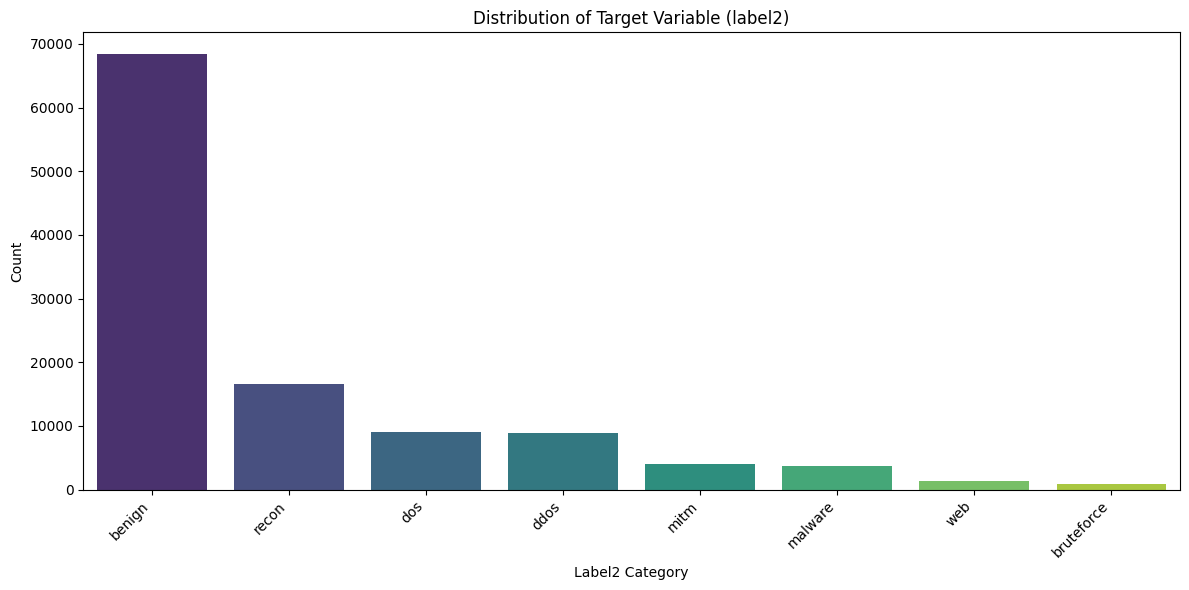
\includegraphics[width=5in]{Images/class_distribution.png}}
			{\rule{5in}{3.5in} % Placeholder -- add file at Images/class_distribution.png
			\\[-3.7in]\centering\textit{\small [Image not yet added: Images/class\_distribution.png]}\\[3.5in]}
	\end{center}
	\caption{Class distribution of the 8-category grouped label (benign plus seven attack categories) in the CIC IIoT 2025 evaluation subset: benign ($\approx$68{,}000), Recon ($\approx$16{,}500), DoS ($\approx$9{,}000), DDoS ($\approx$8{,}800), MITM ($\approx$4{,}000), Malware ($\approx$3{,}700), Web ($\approx$1{,}300), and Bruteforce ($<$1{,}000).}
	\label{fig:class_distribution}
\end{figure}

\textbf{Hardware and Software Environment:} The edge-layer models (GRU and Deep SVDD) were deployed on a simulated edge device using a [Insert Edge Hardware, e.g., Raspberry Pi 4 Model B with 4GB RAM]. As detailed in Section \ref{sec:edge_eval}, device-level latency and throughput benchmarking to date has been performed on the standalone baseline models compared against the proposed ensemble, run in a notebook development environment rather than on constrained edge hardware itself; benchmarking the deployed fused GRU + Deep SVDD ensemble under the same conditions, and repeating both on the target edge hardware, remains an open item noted in Section \ref{sec:limitations_integration}. The cloud-layer components run as a single Python process (a FastAPI application driven by \texttt{asyncio}, with no separate message broker or worker processes): a pre-trained XGBoost classifier and SHAP \texttt{TreeExplainer} for classification and explainability, and a LangChain-based Decision/Escalation Agent pipeline grounded by a FAISS vector store (falling back to a TF-IDF retriever when no embedding API key is configured) for the two LLM fallback touchpoints described in Section \ref{sec:multi_agent}. Because both the classifier and its explainer are tree-based rather than deep-learning models, this cloud tier has no GPU dependency; it was run on commodity CPU-only compute. The language-model calls in the \texttt{openai} configuration used [Insert Model, e.g., \texttt{gpt-4o-mini}] as the underlying LLM.

\textbf{Verification methodology:} In addition to the offline, dataset-driven evaluation of the edge-layer ensemble reported in Section \ref{sec:edge_eval}, the cloud-layer pipeline was verified through two rounds of live testing driven entirely over its two edge-facing HTTP endpoints, i.e. with a test harness playing the role of ``an edge layer,'' independently of this project's own edge-layer implementation (Section \ref{sec:limitations_integration} discusses why this separation was necessary). The first round exercised classification in isolation against a set of hand-crafted, unambiguous attack windows. The second round first performed a systematic grid search of the classifier's confidence boundary across roughly 40 traffic patterns at multiple volumes, then drove the full downstream chain-ladder escalation, edge apply/verification feedback, the final-tier approval gate, benign-state decay scheduling, both LLM fallback triggers, and the RAG self-learning write-back-end to end over HTTP for five representative scenarios. The findings from both rounds are reported in Sections \ref{sec:cloud_eval} and \ref{sec:mas_eval}.

\section{Edge Layer: Anomaly Detection Performance}\label{sec:edge_eval}

The proposed Cascaded Hybrid Ensemble (GRU + Deep SVDD) was benchmarked against eight alternative models trained and evaluated on the same held-out data: four standard supervised tree ensembles (Hist Gradient Boosting, Random Forest, Extra Trees, and the unsupervised Isolation Forest baseline), three classical linear/kernel classifiers (Gaussian Naive Bayes, Logistic Regression, and a Support Vector Classifier), and a standalone Deep SVDD model receiving only the point features, without the GRU's temporal embedding. This last comparison is the ensemble's ablation: it isolates what the GRU's temporal context specifically contributes, holding the Deep SVDD boundary itself fixed.

Table \ref{tb:edge_results} summarizes the detection performance of all nine models. The proposed ensemble achieved the highest score on every reported metric, and by a wide margin over standalone Deep SVDD specifically: accuracy improved by approximately 44.0 percentage points (55.6\% $\to$ 99.61\%), precision by approximately 46.4 points (53.3\% $\to$ 99.65\%), recall by approximately 8.8 points (91.0\% $\to$ 99.77\%), F1 by approximately 32.5 points (67.2\% $\to$ 99.71\%), and ROC-AUC by approximately 54.1 points (45.9\% $\to$ 99.98\%). Because the ensemble and the standalone Deep SVDD figures were produced by separate evaluation pipelines rather than a single controlled ablation run holding every other variable fixed, these deltas are reported here as descriptive rather than as a strictly paired ablation result, consistent with how the underlying evaluation itself qualifies the comparison. The direction and scale of the improvement are nonetheless consistent with the design argument of Section \ref{sec:hybrid_ensemble}: the GRU's temporal embedding gives Deep SVDD a materially richer representation to draw a boundary around than point features alone, particularly for recall, where standalone Deep SVDD's 91.0\% already indicates it detects most attacks in isolation but at the cost of far more false positives (53.3\% precision) than the fused ensemble ever exhibits. Figure \ref{fig:f1_benchmark} presents this same comparison visually, ranking all nine models by F1-score and showing the full five-metric heatmap side by side, which makes the size of the proposed ensemble's margin over every baseline immediately apparent.

\begin{table}[htbp]
\caption{Performance comparison of the proposed GRU + Deep SVDD ensemble against eight baseline models on the same held-out evaluation data.}
\label{tb:edge_results}
\begin{center}
\begin{tabular}{|l|c|c|c|c|}
\hline
\textbf{Model} & \textbf{Accuracy} & \textbf{Precision} & \textbf{Recall} & \textbf{F1-Score} \\
\hline
\textbf{GRU + Deep SVDD Ensemble} & \textbf{0.9961} & \textbf{0.9965} & \textbf{0.9977} & \textbf{0.9971} \\
\hline
Hist Gradient Boosting & 0.964 & 0.991 & 0.937 & 0.963 \\
\hline
Random Forest & 0.961 & 0.988 & 0.932 & 0.959 \\
\hline
Extra Trees & 0.958 & 0.990 & 0.925 & 0.957 \\
\hline
Isolation Forest & 0.886 & 0.904 & 0.864 & 0.883 \\
\hline
Gaussian Naive Bayes & 0.888 & 0.933 & 0.835 & 0.881 \\
\hline
Logistic Regression & 0.891 & 0.969 & 0.807 & 0.881 \\
\hline
Support Vector Classifier & 0.887 & 0.942 & 0.824 & 0.879 \\
\hline
Standalone Deep SVDD & 0.556 & 0.533 & 0.910 & 0.672 \\
\hline
\end{tabular}
\end{center}
\raggedright \textit{*Note: Standalone Deep SVDD receives point features only (no GRU temporal embedding) and constitutes the ablation baseline for the proposed ensemble.}
\end{table}

\begin{figure}[htbp]
	\begin{center}
		\IfFileExists{Images/edge/Fused GRU + Deep SVDD Against Individual Approaches.png}
			{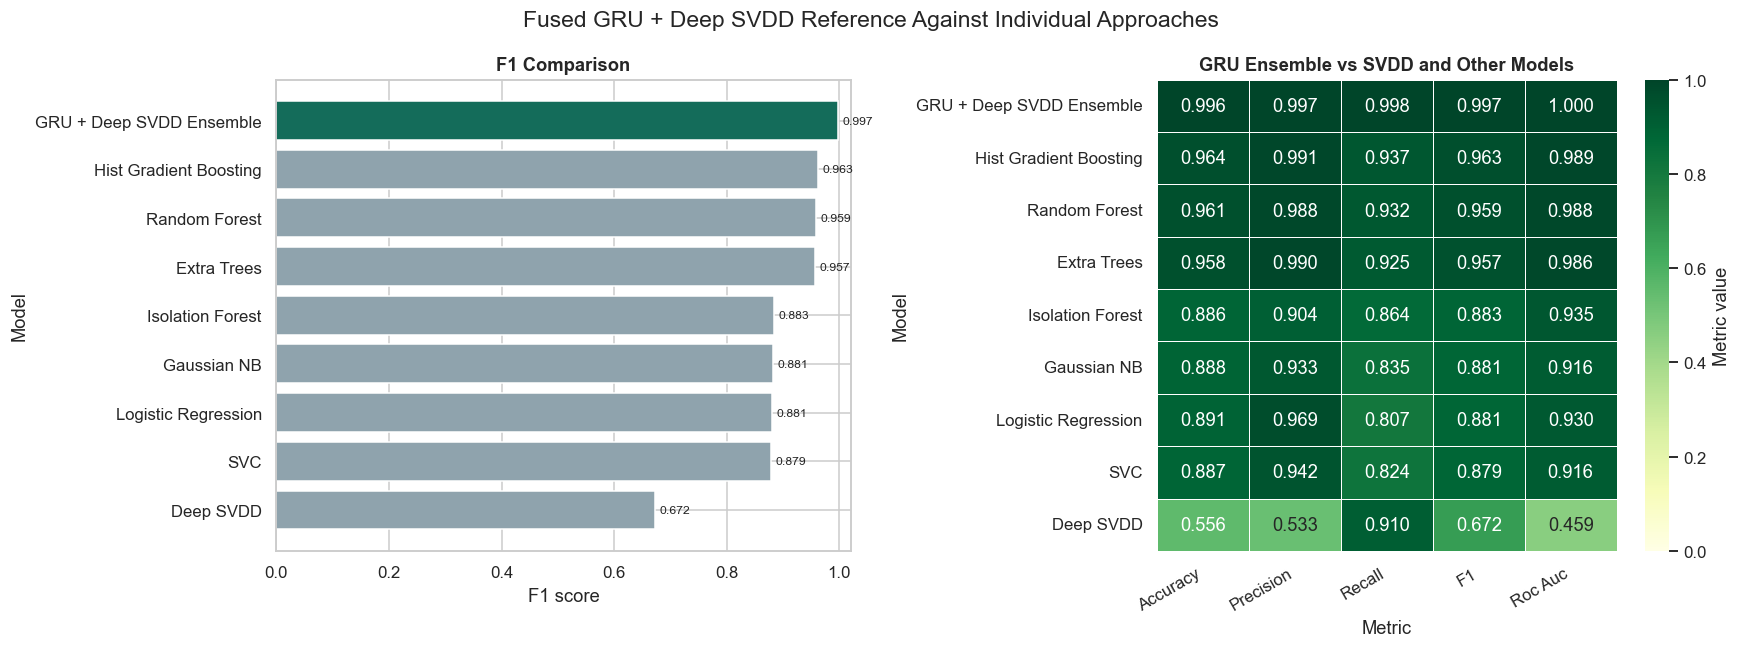
\includegraphics[width=5.5in]{Images/edge/Fused GRU + Deep SVDD Against Individual Approaches.png}}
			{\rule{5.5in}{4cm} % Placeholder -- add file at Images/edge/Fused GRU + Deep SVDD Against Individual Approaches.png
			\\[-4.2cm]\centering\textit{\small [Image not yet added: Images/f1\_benchmark\_comparison.png]}\\[4cm]}
	\end{center}
	\caption{F1-score comparison across all nine models (bar chart), alongside a heatmap of all five metrics per model, corresponding to the figures reported in Table \ref{tb:edge_results}.}
	\label{fig:f1_benchmark}
\end{figure}

Figure \ref{fig:fusion_comparison} isolates this ablation on its own axes, plotting the standalone Deep SVDD baseline against the fused ensemble across all five metrics so that the per-metric size of the fusion benefit-smallest for recall, largest for ROC-AUC-can be read directly rather than reconstructed from the percentage-point deltas above.

\begin{figure}[htbp]
	\begin{center}
		\IfFileExists{Images/edge/What fusion adds over standalone Deep SVDD.png}
			{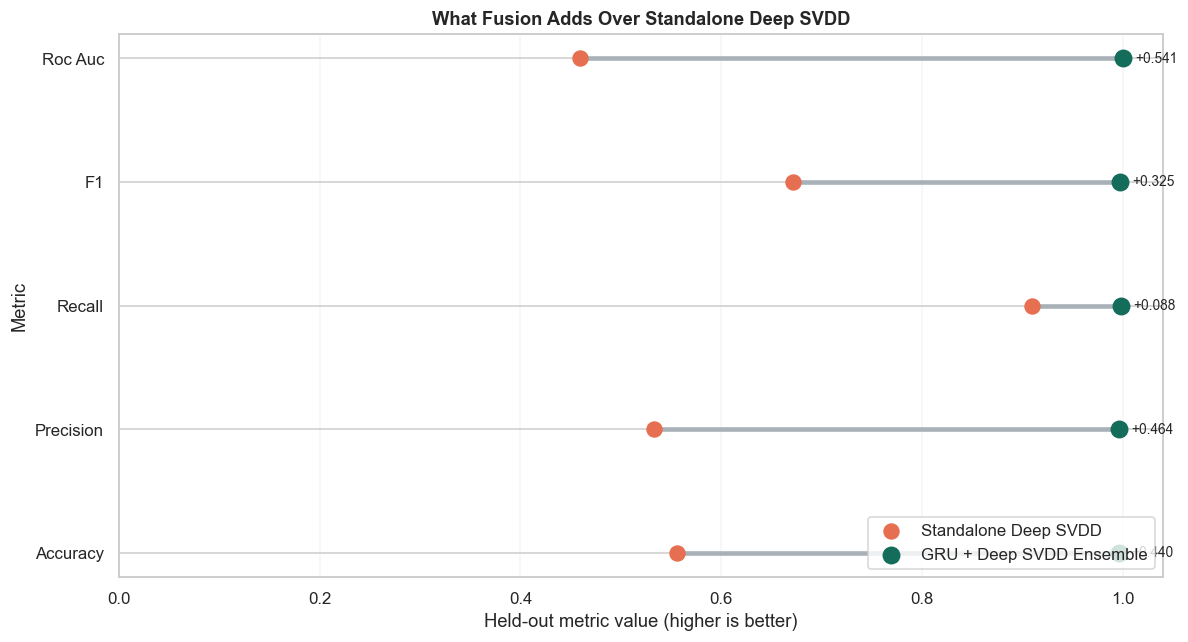
\includegraphics[width=5.5in]{Images/edge/What fusion adds over standalone Deep SVDD.png}}
			{\rule{5.5in}{4cm} % Placeholder -- add file at Images/edge/What fusion adds over standalone Deep SVDD.png
			\\[-4.2cm]\centering\textit{\small [Image not yet added: Images/fusion\_comparison.png]}\\[4cm]}
	\end{center}
	\caption{What fusion adds over standalone Deep SVDD: a per-metric comparison (accuracy, precision, recall, F1, ROC-AUC) between the standalone Deep SVDD baseline and the fused GRU + Deep SVDD ensemble, corresponding to the deltas discussed above.}
	\label{fig:fusion_comparison}
\end{figure}

At its selected operating threshold, the proposed ensemble's detailed classification breakdown on the 9{,}000-sample held-out set (3{,}000 benign, 6{,}000 attack) is reported in Table \ref{tb:edge_confusion} and visualised as a confusion matrix in Figure \ref{fig:confusion_matrix}. Of 3{,}000 benign windows, 21 were incorrectly flagged as attacks (a 0.70\% false-positive rate); of 6{,}000 attack windows, 14 were missed (a 0.23\% false-negative rate).

\begin{table}[htbp]
\caption{Confusion matrix and per-class detection metrics for the proposed GRU + Deep SVDD ensemble at its selected operating threshold.}
\label{tb:edge_confusion}
\centering
\begin{tabular*}{\textwidth}{@{\extracolsep{\fill}}|l|c|c|c|c|}
\hline
\textbf{Class} & \textbf{Precision} & \textbf{Recall} & \textbf{F1-Score} & \textbf{Support} \\
\hline
Normal (benign) & 0.9953 & 0.9930 & 0.9942 & 3{,}000 \\
\hline
Attack & 0.9965 & 0.9977 & 0.9971 & 6{,}000 \\
\hline
\end{tabular*}
\end{table}

\begin{figure}[htbp]
	\begin{center}
		\IfFileExists{Images/edge/Confusion Matrix GRU-SVDD.png}
			{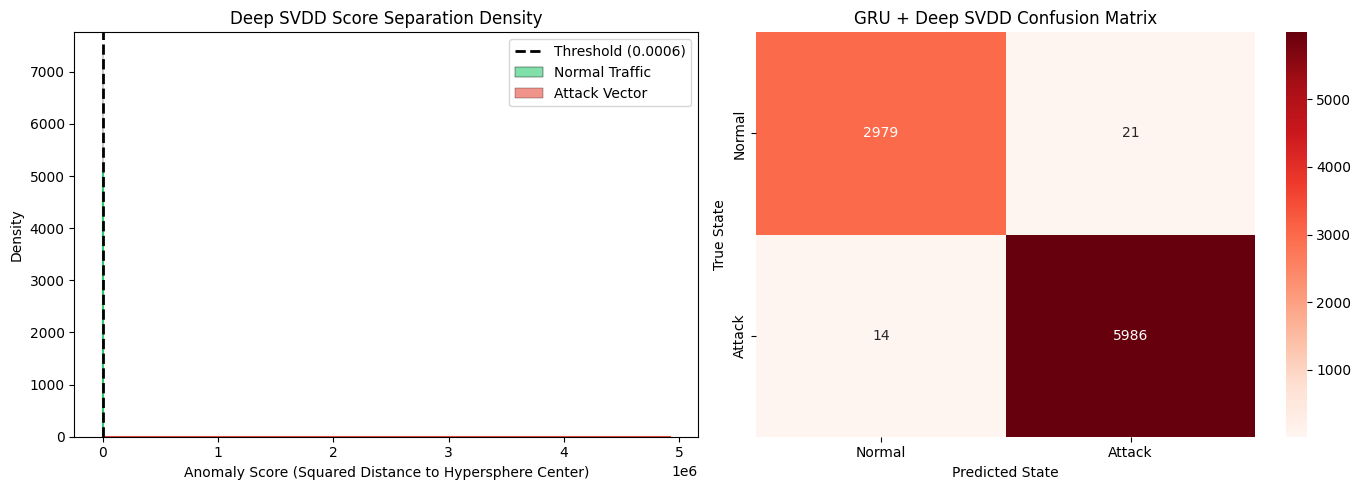
\includegraphics[width=5.5in]{Images/edge/Confusion Matrix GRU-SVDD.png}}
			{\rule{3.5in}{3.5in} % Placeholder -- add file at Images/edge/Confusion Matrix GRU-SVDD.png
			\\[-3.7in]\centering\textit{\small [Image not yet added: Images/confusion\_matrix.png]}\\[3.5in]}
	\end{center}
	\caption{Confusion matrix for the fused GRU + Deep SVDD ensemble at its selected operating threshold, corresponding to the figures reported in Table \ref{tb:edge_confusion}.}
	\label{fig:confusion_matrix}
\end{figure}

The operating threshold itself was selected via the same offline precision-recall/F1 search described in Section \ref{sec:hybrid_ensemble}, applied to the log-normalized distance score $d(v)$; the resulting threshold ($d(v) \approx 0.0006$) sits at the point where the precision and recall curves cross, balancing the two error types rather than minimising either in isolation. Figure \ref{fig:threshold_selection} shows the full basis for this choice: the log-normalized separation between benign and attack scores, the precision/recall/F1 trade-off curve, and the resulting false-positive/false-negative rate trade-off, with the selected threshold marked on each panel.

\begin{figure}[htbp]
	\begin{center}
		\IfFileExists{Images/edge/GRU + Deep SVDD Fused Anomaly_Benign Threshold Selection.png}
			{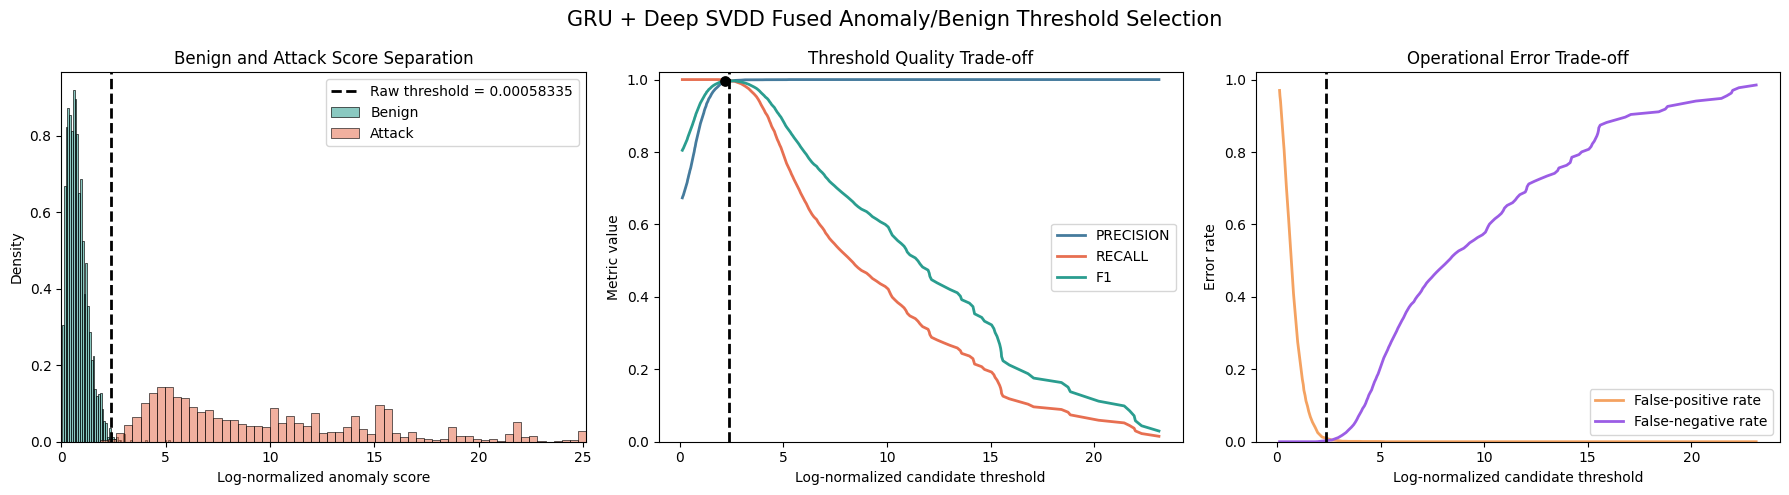
\includegraphics[width=\textwidth]{Images/edge/GRU + Deep SVDD Fused Anomaly_Benign Threshold Selection.png}}
			{\rule{5.5in}{4cm} % Placeholder -- add file at Images/edge/GRU + Deep SVDD Fused Anomaly_Benign Threshold Selection.png
			\\[-4.2cm]\centering\textit{\small [Image not yet added: Images/threshold\_selection.png]}\\[4cm]}
	\end{center}
	\caption{Threshold selection for the fused GRU + Deep SVDD score: benign/attack score separation on a log-normalized scale, the precision/recall/F1 trade-off curve, and the resulting false-positive/false-negative rate trade-off, with the selected operating threshold marked.}
	\label{fig:threshold_selection}
\end{figure}

\textbf{Edge-device hardware constraints.} Predictive quality must ultimately be balanced against the resource budget available on the target edge hardware (Chapter \ref{cha:introduction}). This trade-off was first characterised only for the baseline models evaluated in a notebook development environment: under those notebook conditions, the selected Random Forest configuration (250 trees, maximum depth 18) required 0.57 seconds to fit and scored the held-out batch in 0.0258 seconds, corresponding to approximately 309{,}543 rows per second; Hist Gradient Boosting scored the same batch in 0.0081 seconds (approximately 987{,}822 rows per second); and standalone Deep SVDD scored it in 0.0070 seconds (approximately 1{,}144{,}247 rows per second). These notebook-environment figures cover only the standalone baseline models and say nothing about the fused ensemble's own recurrent-inference and sequence-buffering overhead, nor about behaviour on the constrained target hardware itself, since large tree ensembles such as Random Forest additionally carry a memory and storage cost that a resource-constrained gateway may not be able to absorb regardless of raw throughput.

\textbf{On-device benchmark of the deployed fused ensemble.} The deployed, production GRU--Deep SVDD pipeline (artifact \texttt{gru-svdd-e3d39953d09f}) was subsequently benchmarked directly on a Raspberry Pi-class edge device (4-core ARM Cortex-A76, up to 2.4\,GHz, 8\,GiB RAM), closing part of the open item raised above. For each candidate CPU-thread configuration, 1{,}000 inferences were measured following 50 discarded warm-up runs; Table \ref{tb:edge_hw_benchmark} reports the resulting latency distribution and throughput.

\begin{table}[htbp]
\caption{On-device inference benchmark for the deployed fused GRU + Deep SVDD ensemble on the target Raspberry Pi-class gateway, across candidate CPU-thread configurations (1{,}000 measured inferences after 50 warm-up runs); all latency values are reported in milliseconds.}
\label{tb:edge_hw_benchmark}
\begin{center}
\begin{tabular}{|c|c|c|c|c|c|c|}
\hline
\textbf{Threads} & \textbf{Mean} & \textbf{Median} & \textbf{p95} & \textbf{p99} & \textbf{Max} & \textbf{Throughput (dec/s)} \\
\hline
\textbf{1} & \textbf{2.64} & \textbf{1.45} & \textbf{8.11} & \textbf{10.36} & 36.45 & \textbf{379} \\
\hline
2 & 2.78 & -- & -- & -- & -- & 360 \\
\hline
4 & 2.95 & 1.43 & 11.09 & 13.37 & 31.16 & 339 \\
\hline
\end{tabular}
\end{center}
\raggedright \textit{*Note: only the figures reported for the 1-thread and 4-thread configurations were directly available from the underlying benchmark run; the 2-thread row reports mean latency and throughput only.}
\end{table}

A single CPU thread gave the best balance of latency and throughput ($\approx$379 decisions/second at a mean latency of 2.64\,ms); two and four threads were both slower (360 and 339 decisions/second respectively), indicating that thread-management overhead outweighs any parallelism this comparatively compact model can exploit. Model initialisation took approximately 1.05 seconds with cached artifacts and approximately 4.28 seconds on a cold load, and the Python inference process reached a peak of approximately 332\,MiB RAM. Measured against the 2-second and 10-second scoring intervals the edge layer operates on (Chapter 3, Methodology), even the four-thread configuration's worst-case p99 latency (13.37\,ms) leaves substantial headroom, indicating that CPU and memory budget are not the binding constraint on scoring frequency for this ensemble on this hardware class.

Separately, the exported production model reports a detection quality of 0.913 F1, 99.49\% precision, 84.29\% recall, a ROC-AUC of 0.939, and a 1.97\% benign false-positive rate. These figures are noticeably weaker on recall than the 0.9971 F1 (99.65\% precision, 99.77\% recall) reported for the same ensemble on the notebook-evaluated held-out set in Table \ref{tb:edge_confusion}, and the gap is not yet reconciled: it may reflect a different train/evaluation split, a quantised or otherwise reduced export of the model used for the hardware benchmark, or a different operating threshold than the one selected in Figure \ref{fig:threshold_selection}. This discrepancy is noted here rather than resolved, consistent with this report's practice of surfacing rather than silently smoothing over inconsistencies between evaluation runs, and is carried forward as an open item in Section \ref{sec:limitations_integration}.

\section{Cloud Layer: Threat Classification and XAI}\label{sec:cloud_eval}

The cloud tier's classifier is trained against 76 fine-grained attack labels, grouped by summed class probability into the eight buckets described in Section \ref{sec:cloud_classification} (\texttt{benign}, \texttt{ddos}, \texttt{port\_scan}, \texttt{bruteforce}, \texttt{mirai\_botnet}, \texttt{lateral\_movement}, \texttt{exfiltration}, \texttt{unhandled\_attack}). Of the 30 numeric features the classifier expects, only a subset can be populated from data the edge layer actually forwards, because the edge sends connection-log-style aggregates rather than the packet-level captures (TCP window size, time-to-live statistics, maximum segment size, IP flags) the classifier was originally trained on; the remaining features are populated with a fixed placeholder value rather than left undefined. This is a structural mismatch between the granularity the model expects and the granularity the pipeline can supply, not a bug in either component individually, and it is the dominant factor behind the findings below.

\textbf{Offline validation on native features.} Before considering what happens when the edge layer supplies an incomplete feature vector, it is worth establishing whether the classification approach is sound at all when given the dataset's complete, native feature set. Table \ref{tb:offline_validation} reports validation performance for five candidate classifiers trained and evaluated at the 8-category grouped-label granularity (\texttt{label2}: benign plus the seven attack categories introduced in this chapter's Experimental Setup section above) on the same CIC IIoT 2025 subset. XGBoost was the strongest of the five, with 94.55\% accuracy and a macro F1-score of 92.60\%, ahead of Random Forest (93.09\%, 91.12\%), KNeighbors (92.83\%, 88.45\%), and Decision Tree (92.32\%, 89.49\%); GaussianNB was markedly weaker on every metric (76.47\% accuracy, 53.86\% macro F1), consistent with a linear-boundary model struggling against the non-linear decision boundaries a tree ensemble captures naturally. Figure \ref{fig:validation_accuracy} plots this same accuracy ranking, making GaussianNB's gap from the other four candidates visually unambiguous.

\begin{table}[htbp]
\caption{Offline validation performance of five candidate classifiers at the 8-category grouped-label granularity, evaluated on the CIC IIoT 2025 dataset with its complete native feature set.}
\label{tb:offline_validation}
\begin{center}
\begin{tabular}{|l|c|c|c|c|}
\hline
\textbf{Model} & \textbf{Accuracy} & \textbf{Macro Precision} & \textbf{Macro Recall} & \textbf{Macro F1-score} \\
\hline
\textbf{XGBoost} & \textbf{0.9455} & \textbf{0.9702} & 0.8887 & \textbf{0.9260} \\
\hline
Random Forest & 0.9309 & 0.9419 & 0.8842 & 0.9112 \\
\hline
KNeighbors & 0.9283 & 0.9337 & 0.8436 & 0.8845 \\
\hline
Decision Tree & 0.9232 & 0.9183 & 0.8735 & 0.8949 \\
\hline
GaussianNB & 0.7647 & 0.5947 & 0.5894 & 0.5386 \\
\hline
\end{tabular}
\end{center}
\end{table}

\begin{figure}[htbp]
	\begin{center}
		\IfFileExists{Images/validation_accuracy_comparison.png}
			{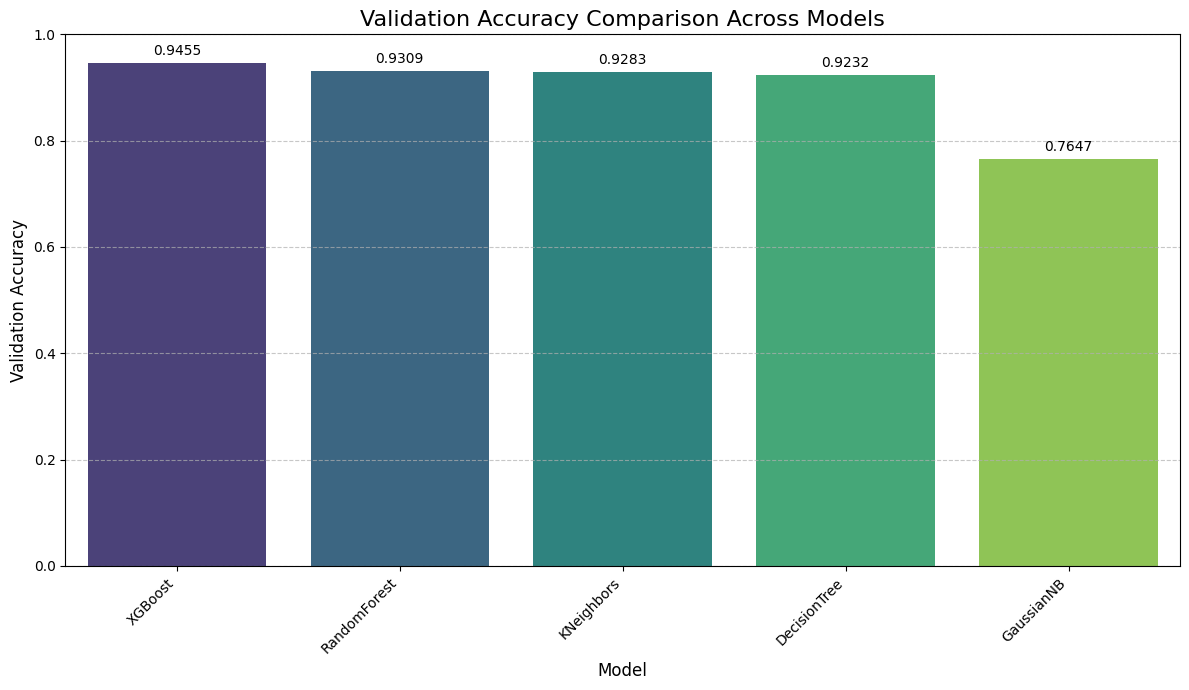
\includegraphics[width=5in]{Images/validation_accuracy_comparison.png}}
			{\rule{5in}{3.5in} % Placeholder -- add file at Images/validation_accuracy_comparison.png
			\\[-3.7in]\centering\textit{\small [Image not yet added: Images/validation\_accuracy\_comparison.png]}\\[3.5in]}
	\end{center}
	\caption{Validation accuracy comparison across the five candidate classifiers reported in Table \ref{tb:offline_validation}.}
	\label{fig:validation_accuracy}
\end{figure}

This result is a useful counterpoint to the live findings that follow: it indicates that XGBoost, given the features it was actually designed around, discriminates this dataset's attack categories well. The gap between this offline result and the live, edge-simulated findings below is consequently attributable to the feature-completeness gap described above, not to the underlying classification approach being unsound. XGBoost's macro recall (88.87\%) was nonetheless the weakest of its four reported metrics, and not uniformly so across classes: two of the eight categories showed recall as low as 77.86\% and 81.72\% respectively even with the complete native feature set, indicating that some attack categories are harder to separate from the majority-benign traffic than others regardless of feature completeness, a caveat worth carrying forward alongside the feature-gap explanation rather than treating the offline result as an unqualified upper bound.

The systematic confidence-boundary probe described in this chapter's Experimental Setup section above-roughly 40 traffic patterns evaluated against the live classifier across a range of record volumes per window-produced the following findings, each independently reproduced rather than observed once:

\begin{itemize}
	\item \textbf{False negatives at high confidence.} Port scans, SSH/Telnet dictionary brute-force attempts, and Mirai-style outbound scanning traffic were classified as \texttt{benign} at 90--98\% confidence across every volume tested (50 to 20,000 records per window)-never once crossing into a detected state.
	\item \textbf{False positives at high confidence.} A purely legitimate, heavy but ordinary HTTPS session was classified \texttt{ddos} at 55\% confidence. This was reproduced end to end through the full downstream pipeline, and it dispatched real containment actions (flood hardening and rate limiting, \texttt{NET-02} + \texttt{NET-01}) against a device that was never actually under attack.
	\item \textbf{Confidence is non-monotonic with attack volume.} A SYN flood crossed the confidence gate at 50 records per window; the same attack pattern at 300 records did not; at 1,000 or more records it flipped to a confidently \texttt{benign} classification. Confidence at this classifier's output is consequently not a reliable proxy for attack severity, or even attack presence, in this pipeline.
	\item \textbf{The fine-grained label is frequently wrong even when the grouped bucket's gate is crossed.} UDP floods were classified into fine-grained labels such as \texttt{unhandled\_attack} or \texttt{web\_sql-injection} rather than any \texttt{ddos}-family label, even in cases where a large-payload flood happened to land on a correct \texttt{ddos} fine label.
\end{itemize}

Taken together, these findings indicate that classification accuracy on real-world, connection-log-shaped input is the dominant limitation of the cloud tier as currently integrated, in both directions: attacks are missed, and benign traffic is acted against. This is discussed further, alongside its likely cause and possible remediations, in Section \ref{sec:limitations_integration}.

Crucially, the classification is still passed through a SHAP explainer regardless of its correctness, computed against the predicted fine-grained label. The top-3 contributing features by $|\phi_i|$ (Equation \ref{e:shap}) are translated into short plain-English statements-for example, describing a high count of unanswered SYN packets as evidence pushing the classification toward a particular attack class-and this translated attribution, rather than the raw SHAP vector, is what is passed to the Dashboard Reporting Agent and to either LLM fallback agent when one is consulted. The explainer's correctness is bounded by the classifier's own correctness: SHAP faithfully explains \textit{why} the model produced a given output, but on the evidence above it cannot compensate for the model being asked to classify against features it was never actually given.

\subsection{Explanation-Quality Metrics}\label{sec:xai_eval}

Because the healing pipeline consumes SHAP attributions as first-class evidence rather than as an advisory overlay, the attributions were evaluated as a subsystem in their own right, in addition to the correctness deletion curve reported in Section \ref{sec:cloud_classification} (Figure \ref{fig:correctness_deletion}, AUPC = 0.1264). The four metrics reported below assess complementary properties: completeness (do the attributions add up to what the model actually output?), continuity (do neighbouring inputs receive comparable explanations?), contrastivity (do different attack classes rely on distinguishably different feature sets?), compactness (how few features are needed to account for most of the attribution mass?), and global feature importance (which features drive one representative class overall?).

\textbf{Completeness (additivity).} SHAP's defining property is that the model's output for a given sample should equal the baseline prediction plus the sum of the per-feature contributions, so a residual close to zero indicates that the returned explanation faithfully reproduces the model output rather than approximating it. Figure \ref{fig:xai_completeness} plots the distribution of absolute residuals $|f(x) - (\text{base value} + \sum_i \phi_i)|$ across the evaluation set. The values are concentrated at an extremely small scale (on the order of $10^{-6}$), with virtually the entire distribution below $5 \times 10^{-6}$, which is strong evidence that the SHAP implementation used here is numerically complete and that the summed contributions reconstruct the raw model output with negligible error.

\begin{figure}[htbp]
	\begin{center}
		\IfFileExists{Images/xai_evaluation/completeness_residuals.jpeg}
			{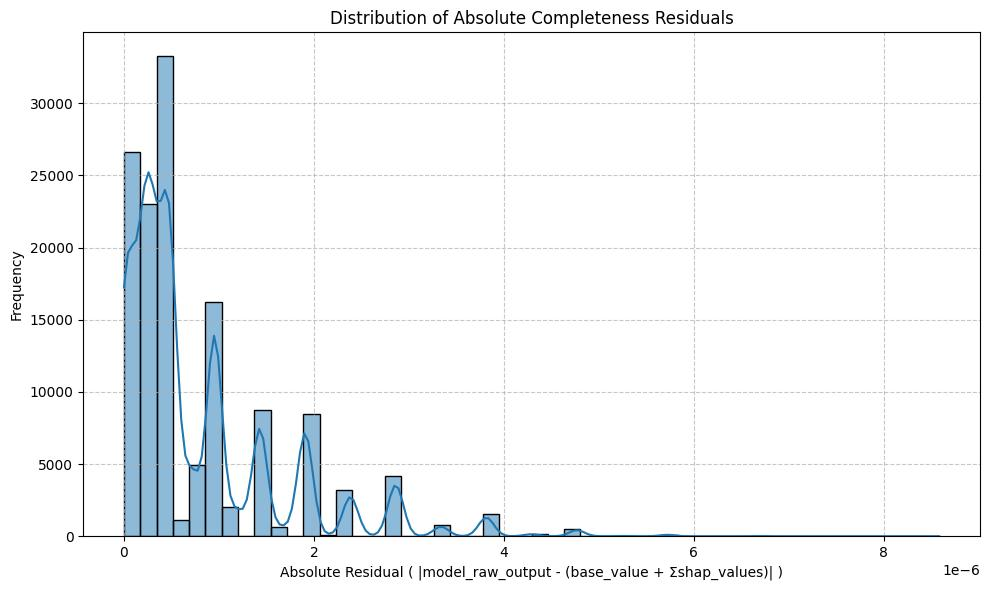
\includegraphics[width=5.5in]{Images/xai_evaluation/completeness_residuals.jpeg}}
			{\rule{5.5in}{3in}
			\\[-3.2cm]\centering\textit{\small [Image not yet added: Images/xai\_evaluation/completeness\_residuals.jpeg]}\\[3in]}
	\end{center}
	\caption{Distribution of absolute completeness residuals, $|f(x) - (\text{base value} + \sum_i \phi_i)|$, across the evaluation set. The residuals are concentrated at the $10^{-6}$ scale, confirming that the SHAP attributions returned by the pipeline reconstruct the raw model output to within numerical noise.}
	\label{fig:xai_completeness}
\end{figure}

\textbf{Continuity (explanation stability).} Continuity measures the average absolute change in SHAP values between comparable or neighbouring samples, capturing whether small input variations produce correspondingly small attribution changes rather than arbitrary shifts. The average continuity score on this classifier is 0.7787 (Figure \ref{fig:xai_continuity}), with the histogram showing that per-sample explanation changes span a range rather than being uniformly near zero. This indicates moderate-to-good continuity: attributions are stable in bulk, but not perfectly so, and some neighbouring windows do receive noticeably different attributions. This is expected near classifier decision boundaries and in regions where network-traffic behaviour changes abruptly between windows, and it is consistent with the non-monotonic-confidence finding reported earlier in this section: where the classifier's own output shifts sharply with small input changes, its explanations shift with it.

\begin{figure}[htbp]
	\begin{center}
		\IfFileExists{Images/xai_evaluation/continuity_distribution.jpeg}
			{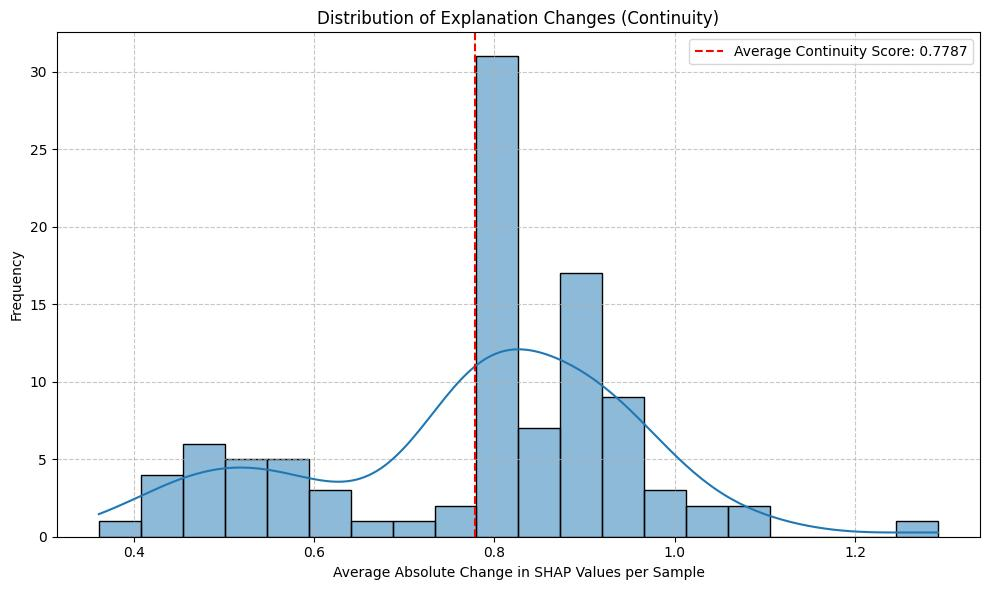
\includegraphics[width=5.5in]{Images/xai_evaluation/continuity_distribution.jpeg}}
			{\rule{5.5in}{3in}
			\\[-3.2cm]\centering\textit{\small [Image not yet added: Images/xai\_evaluation/continuity\_distribution.jpeg]}\\[3in]}
	\end{center}
	\caption{Distribution of per-sample explanation changes (continuity). The dashed line marks the average continuity score of 0.7787; the spread indicates moderate-to-good stability, with the tail representing samples near classifier decision boundaries where attributions shift more sharply.}
	\label{fig:xai_continuity}
\end{figure}

\textbf{Contrastivity (class discrimination).} Contrastivity measures the Jaccard distance between the sets of top-10 influential features for each pair of predicted classes: a value of 0.00 means both classes rely on identical top-10 feature sets, while 1.00 means the two classes share no top-10 features at all, so larger values indicate more class-specific explanations. Figure \ref{fig:xai_contrastivity} shows the resulting pairwise heatmap over the eight grouped labels. Most off-diagonal values sit between 0.46 and 0.75, so the classifier's explanations are largely contrastive across attack families. The one notable exception is the \texttt{ddos}--\texttt{recon} pair at 0.18, which indicates substantial overlap in top-attributed features between DDoS and reconnaissance windows-plausible given that both classes are dominated by network-volume and packet-pattern indicators, and worth targeted feature-overlap and confusion analysis. The highest observed distances (0.75) occur for multiple pairs, including \texttt{benign}--\texttt{bruteforce}, \texttt{benign}--\texttt{dos}, \texttt{benign}--\texttt{web}, \texttt{dos}--\texttt{mitm}, \texttt{malware}--\texttt{mitm}, and \texttt{mitm}--\texttt{web}, indicating that these class pairs are being explained through effectively disjoint feature sets.

\begin{figure}[htbp]
	\begin{center}
		\IfFileExists{Images/xai_evaluation/contrastivity_jaccard.jpeg}
			{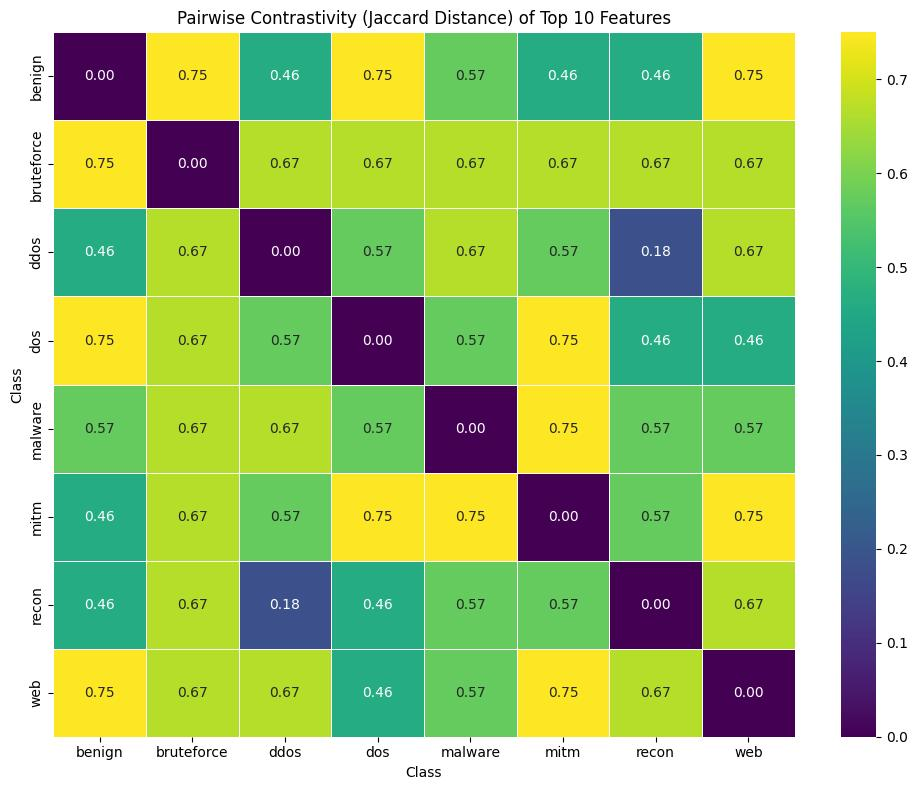
\includegraphics[width=5in]{Images/xai_evaluation/contrastivity_jaccard.jpeg}}
			{\rule{5in}{4in}
			\\[-4.2cm]\centering\textit{\small [Image not yet added: Images/xai\_evaluation/contrastivity\_jaccard.jpeg]}\\[4in]}
	\end{center}
	\caption{Pairwise contrastivity (Jaccard distance) between the top-10 influential features of each pair of predicted classes. Higher values indicate more class-specific explanations; the \texttt{ddos}--\texttt{recon} entry at 0.18 is the main low-contrastivity outlier and is flagged for targeted feature-overlap analysis.}
	\label{fig:xai_contrastivity}
\end{figure}

\textbf{Compactness.} For each sample, the number of features $k$ needed to account for 90\% of the total absolute attribution mass was computed after sorting features by $|\phi_i|$. The average across the evaluation set is $k \approx 9.13$: although the classifier consumes a 30-feature vector, roughly nine features usually explain the bulk of any given prediction. This is directly useful for the downstream healing pipeline, since the top-3 statements passed to the Dashboard Reporting Agent and the LLM fallback agents (Section \ref{sec:multi_agent}) are drawn from precisely this concentrated head of the attribution ranking rather than from a diffuse feature cloud.

\textbf{Global feature importance for the benign class.} Figure \ref{fig:xai_shap_benign} reports the mean absolute SHAP value per feature for the \texttt{benign} output across the evaluation set, expressing global importance magnitude but not direction. The leading features are \path{network_packet-size_min}, \path{network_packets_all_count}, \path{network_window-size_min}, \path{network_ip-length_min}, and \path{network_window-size_max}, followed by \path{network_ports_dst_count}, \path{network_ips_all_count}, and \path{log_data-types}. The \texttt{benign} decision is therefore shaped predominantly by packet-size, packet-count, TCP-window, and IP-length behaviour, which is plausible for traffic classification given that benign traffic typically has a characteristic distribution of flow sizes, packet volumes, and protocol-level properties. Two caveats apply. First, global importance does not establish causality, and the bar chart does not indicate whether a high or low value of each feature increases or decreases the probability of the \texttt{benign} class; per-sample directional plots are the appropriate instrument for that question. Second, this ranking must be read against the granularity mismatch flagged earlier in this section: several of the leading features are precisely the packet-level signals the current edge layer does not natively forward, so the very features on which the model relies most for a \texttt{benign} verdict are the ones most exposed to placeholder-value inference at runtime.

\begin{figure}[htbp]
	\begin{center}
		\IfFileExists{Images/xai_evaluation/shap_importance_benign.jpeg}
			{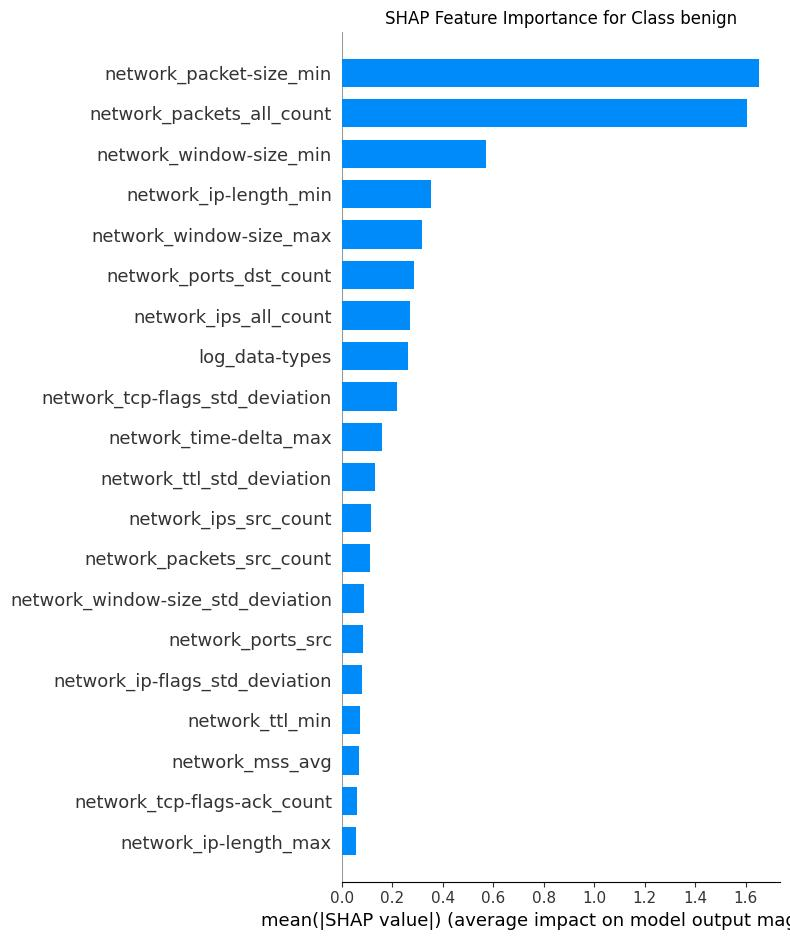
\includegraphics[width=5in]{Images/xai_evaluation/shap_importance_benign.jpeg}}
			{\rule{5in}{4in}
			\\[-4.2cm]\centering\textit{\small [Image not yet added: Images/xai\_evaluation/shap\_importance\_benign.jpeg]}\\[4in]}
	\end{center}
	\caption{Mean absolute SHAP value per feature for the \texttt{benign} class across the evaluation set. Packet-size, packet-count, TCP-window, and IP-length features dominate the \texttt{benign} decision; several of these are also the packet-level signals most affected by the edge-side granularity mismatch discussed in this section.}
	\label{fig:xai_shap_benign}
\end{figure}

\textbf{Per-class global importance across the seven attack families.} The same mean-$|\phi_i|$ ranking was computed for each of the seven attack-class outputs; the results are shown as a grid in Figure \ref{fig:xai_importance_attacks}. Four of the seven classes-\texttt{ddos}, \texttt{dos}, \texttt{malware}, and \texttt{recon}-are led by \path{network_packets_all_count}, indicating that the classifier's top signal for all four is total-volume-per-window rather than any structural fingerprint distinguishing them from one another. This is the same overlap flagged by the contrastivity heatmap (Figure \ref{fig:xai_contrastivity}), where the smallest non-diagonal Jaccard distance was recorded between \texttt{ddos} and \texttt{recon} at 0.18, and it is the most likely explanatory cause of the fine-grained-label errors reported earlier in this section (UDP floods landing on \texttt{unhandled\_attack} or \texttt{web\_sql-injection} rather than a \texttt{ddos}-family label). The remaining three classes are distinguished by different leading features: \texttt{bruteforce} is led by \path{network_time-delta_max}, consistent with the paced, retry-driven timing signature of dictionary attacks; \texttt{mitm} by \path{network_packet-size_min}, consistent with the small, manipulated packets characteristic of man-in-the-middle interception; and \texttt{web} by \path{network_ttl_max}, consistent with the extra routing hops incurred by many web-application attack paths. Log-level features (for example \path{log_data-types}) appear in the top-20 for most classes but rarely near the top, reflecting the classifier's overall bias toward network-layer signals over application-log signals on this feature schema.

\begin{figure}[htbp]
	\centering
	\begin{subfigure}[t]{0.48\textwidth}
		\centering
		\IfFileExists{Images/xai_evaluation/shap_importance_ddos.jpeg}
			{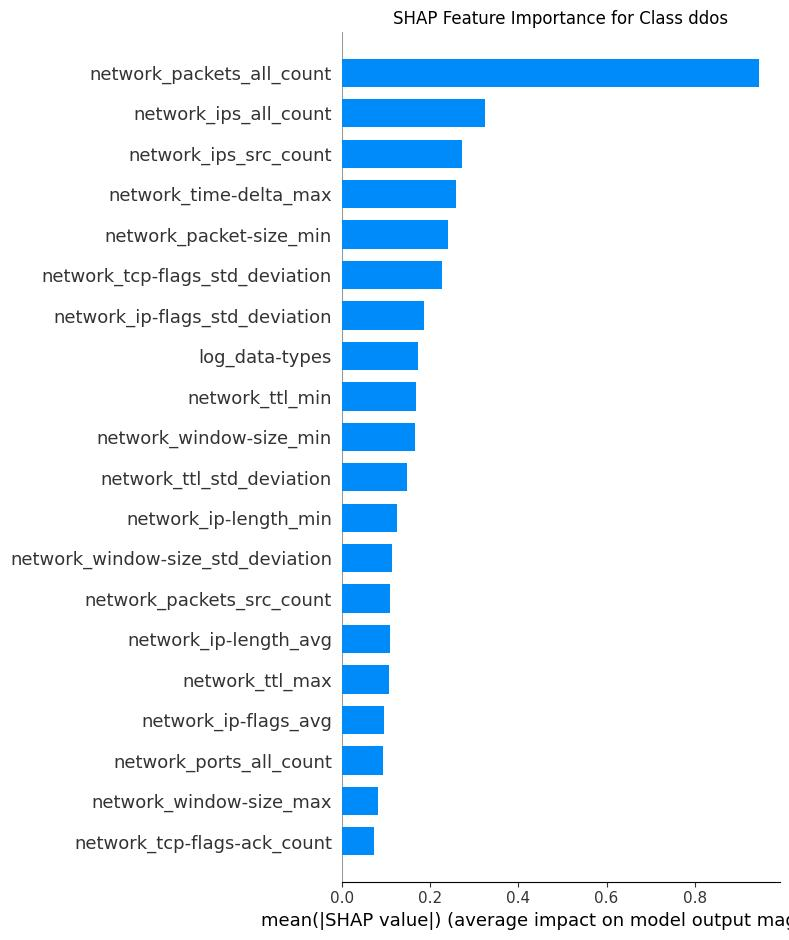
\includegraphics[width=\linewidth]{Images/xai_evaluation/shap_importance_ddos.jpeg}}
			{\rule{\linewidth}{2in}}
		\caption{\texttt{ddos}}
	\end{subfigure}
	\hfill
	\begin{subfigure}[t]{0.48\textwidth}
		\centering
		\IfFileExists{Images/xai_evaluation/shap_importance_dos.jpeg}
			{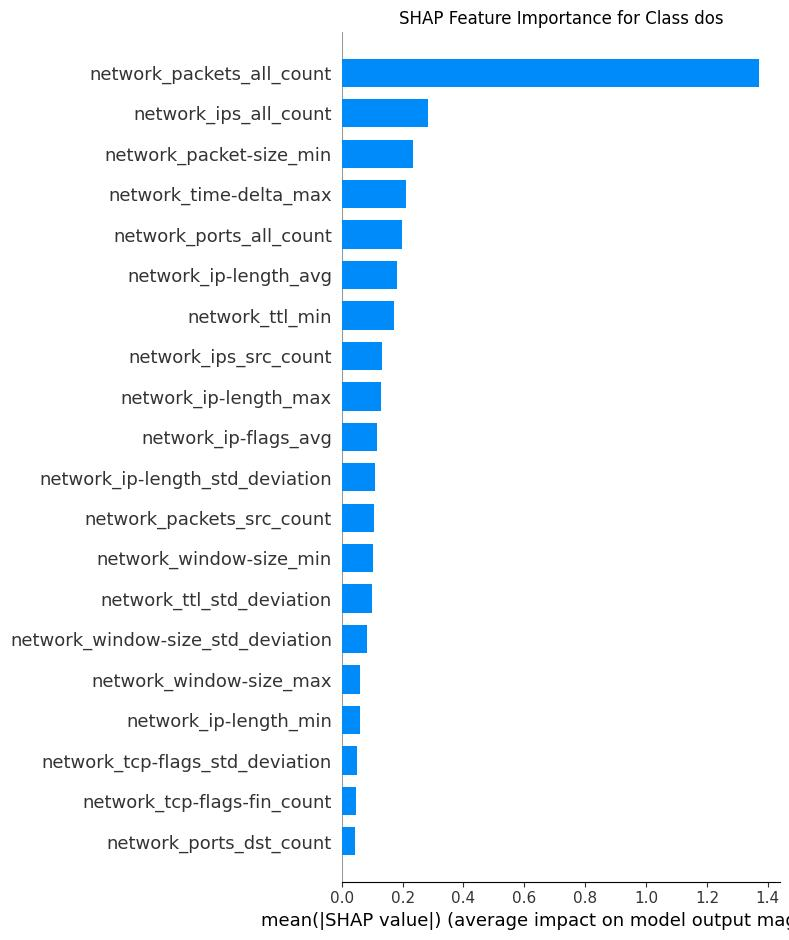
\includegraphics[width=\linewidth]{Images/xai_evaluation/shap_importance_dos.jpeg}}
			{\rule{\linewidth}{2in}}
		\caption{\texttt{dos}}
	\end{subfigure}

	\vspace{0.5em}

	\begin{subfigure}[t]{0.48\textwidth}
		\centering
		\IfFileExists{Images/xai_evaluation/shap_importance_recon.jpeg}
			{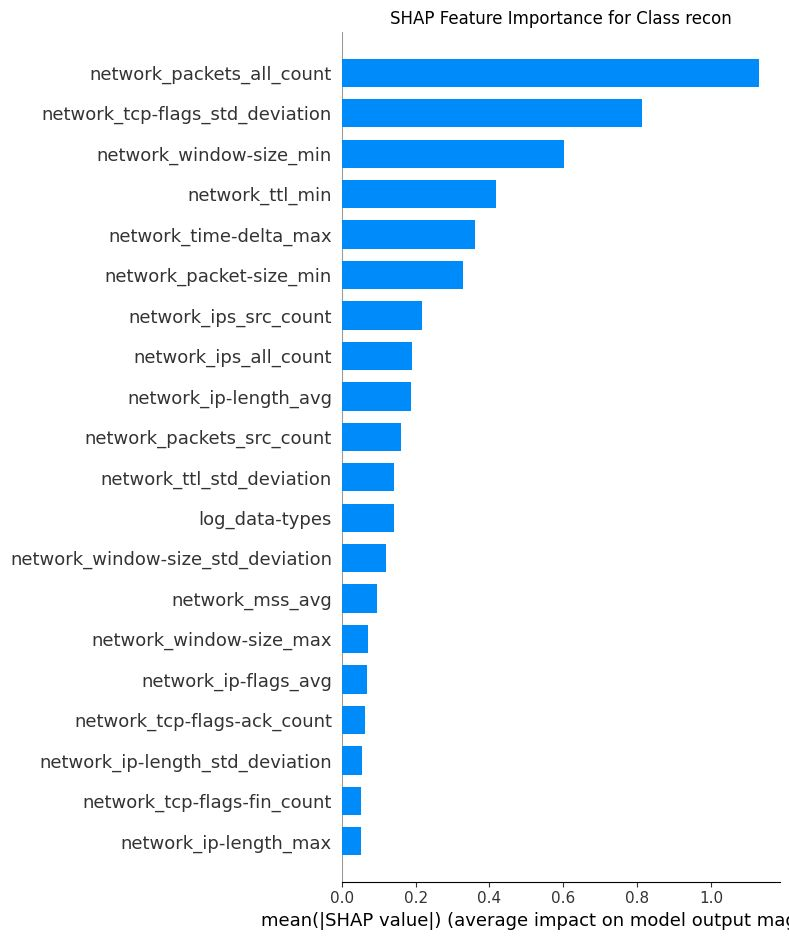
\includegraphics[width=\linewidth]{Images/xai_evaluation/shap_importance_recon.jpeg}}
			{\rule{\linewidth}{2in}}
		\caption{\texttt{recon}}
	\end{subfigure}
	\hfill
	\begin{subfigure}[t]{0.48\textwidth}
		\centering
		\IfFileExists{Images/xai_evaluation/shap_importance_malware.jpeg}
			{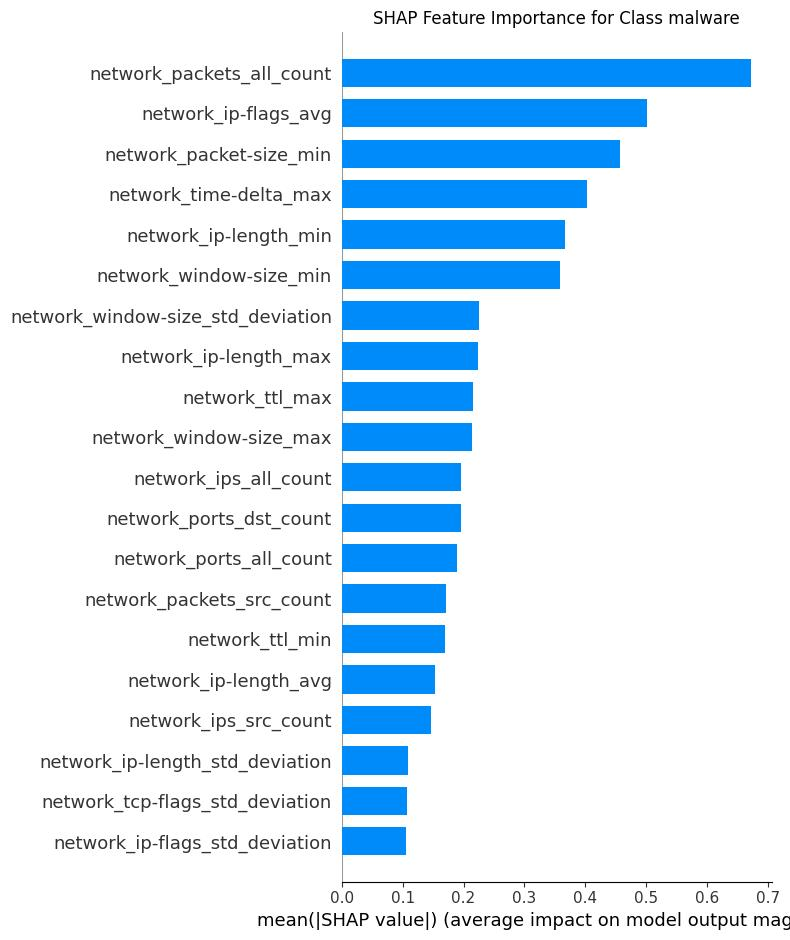
\includegraphics[width=\linewidth]{Images/xai_evaluation/shap_importance_malware.jpeg}}
			{\rule{\linewidth}{2in}}
		\caption{\texttt{malware}}
	\end{subfigure}
	\caption{Mean absolute SHAP value per feature (top-20) for the four volume-led attack-class outputs. All four are led by \texttt{network\_packets\_all\_count}, consistent with the low pairwise-contrastivity outlier flagged in Figure \ref{fig:xai_contrastivity}.}
	\label{fig:xai_importance_attacks}
\end{figure}

\begin{figure}[htbp]\ContinuedFloat
	\centering
	\begin{subfigure}[t]{0.32\textwidth}
		\centering
		\IfFileExists{Images/xai_evaluation/shap_importance_bruteforce.jpeg}
			{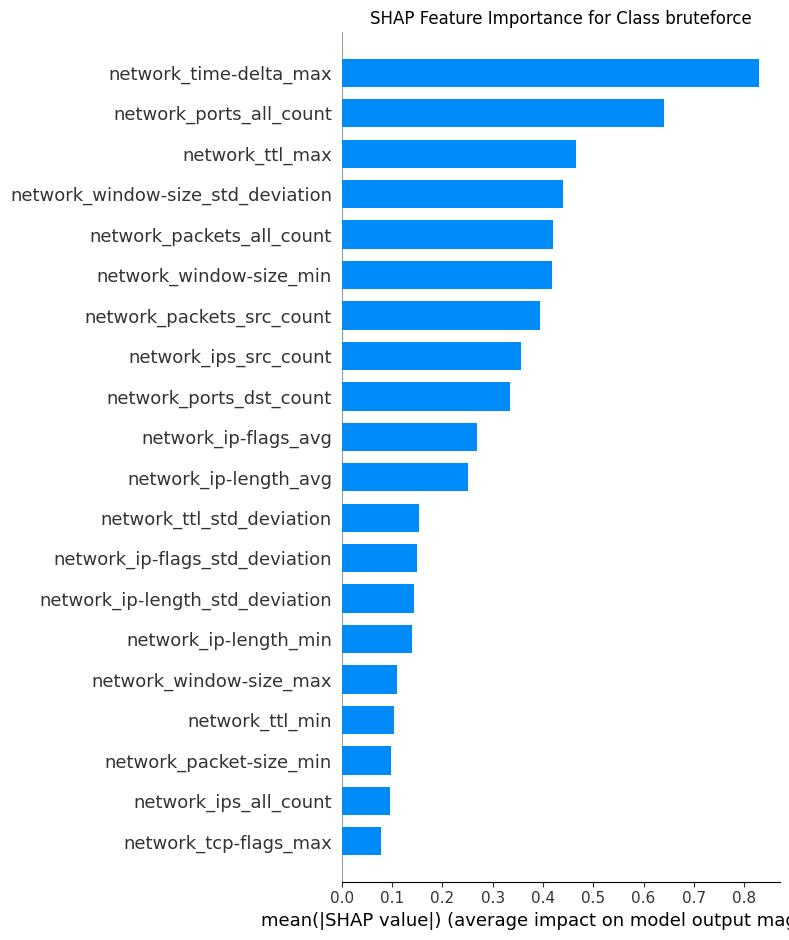
\includegraphics[width=\linewidth]{Images/xai_evaluation/shap_importance_bruteforce.jpeg}}
			{\rule{\linewidth}{2in}}
		\caption{\texttt{bruteforce}}
	\end{subfigure}
	\hfill
	\begin{subfigure}[t]{0.32\textwidth}
		\centering
		\IfFileExists{Images/xai_evaluation/shap_importance_mitm.jpeg}
			{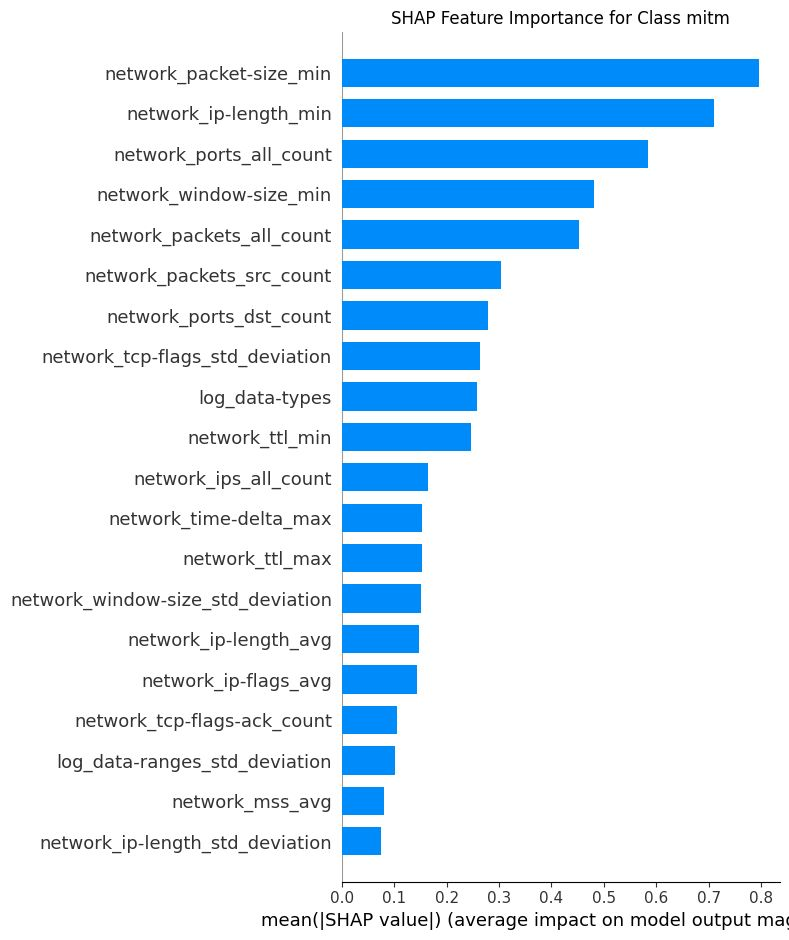
\includegraphics[width=\linewidth]{Images/xai_evaluation/shap_importance_mitm.jpeg}}
			{\rule{\linewidth}{2in}}
		\caption{\texttt{mitm}}
	\end{subfigure}
	\hfill
	\begin{subfigure}[t]{0.32\textwidth}
		\centering
		\IfFileExists{Images/xai_evaluation/shap_importance_web.jpeg}
			{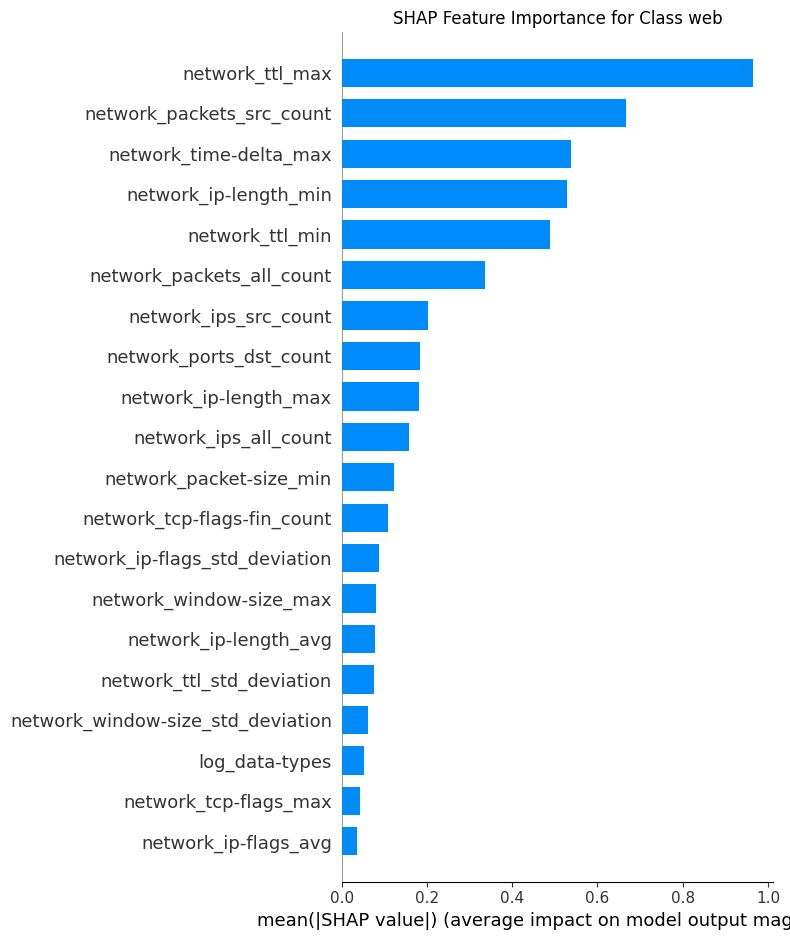
\includegraphics[width=\linewidth]{Images/xai_evaluation/shap_importance_web.jpeg}}
			{\rule{\linewidth}{2in}}
		\caption{\texttt{web}}
	\end{subfigure}
	\caption{Mean absolute SHAP value per feature (top-20) for the three distinct-signature attack-class outputs. \texttt{bruteforce}, \texttt{mitm}, and \texttt{web} are distinguished by timing, small-packet, and TTL-based leading features respectively.}
	\label{fig:xai_importance_attacks_distinct}
\end{figure}

\FloatBarrier

\textbf{Directional analysis via SHAP summary plots.} The bar-chart importance ranking captures magnitude but not the direction in which each feature pushes the class output, and does not reveal whether the relationship between feature value and SHAP contribution is monotonic or not. Figure \ref{fig:xai_summary_attacks} shows the corresponding SHAP summary (beeswarm) plots for the same seven classes: each point represents one sample-feature pair, its horizontal position is the SHAP value contributed by that feature for that sample, and its colour encodes the raw feature value from low (blue) to high (red). Positive SHAP values on the horizontal axis push the model toward the class in question and negative values push it away, so a feature whose high-value points cluster on the right supports the class when observed at a high value, and one whose high-value points cluster on the left opposes it. Two systematic patterns emerge across the attack classes. First, the beeswarms for the four volume-led classes (\texttt{ddos}, \texttt{dos}, \texttt{malware}, \texttt{recon}) show a long red tail of \path{network_packets_all_count} points on the positive side, confirming that high packet counts per window push the model toward each of these attack labels as expected, but also that the same directional signal is being reused for all four. Second, several features show pronounced non-linearity: for \texttt{mitm}, both very-low and moderate values of \path{network_packet-size_min} can produce large positive SHAP values, indicating that the model does not treat this feature as a simple threshold. The wide horizontal spreads visible on the top-ranked features across every class are also the direct empirical explanation for the moderate continuity score reported earlier (0.7787, Figure \ref{fig:xai_continuity}): where a single feature can contribute across a broad SHAP range depending on its raw value, small input differences will produce correspondingly wider attribution differences than they would for a strictly monotonic classifier.

\begin{figure}[htbp]
	\centering
	\begin{subfigure}[t]{0.48\textwidth}
		\centering
		\IfFileExists{Images/xai_evaluation/shap_summary_ddos.jpeg}
			{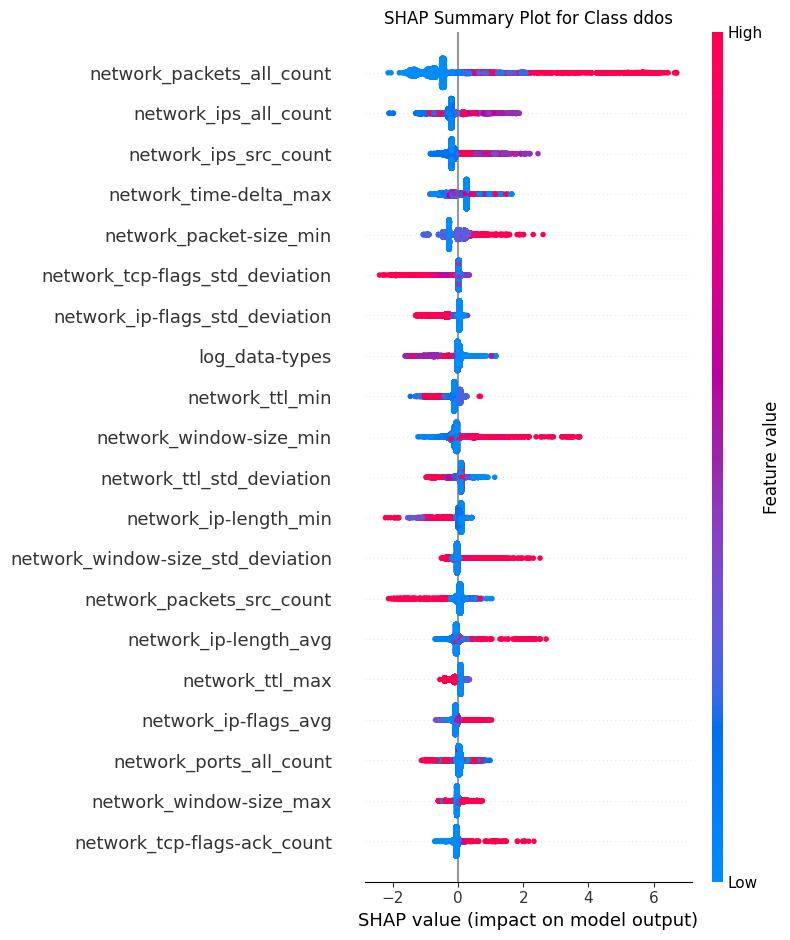
\includegraphics[width=\linewidth]{Images/xai_evaluation/shap_summary_ddos.jpeg}}
			{\rule{\linewidth}{2in}}
		\caption{\texttt{ddos}}
	\end{subfigure}
	\hfill
	\begin{subfigure}[t]{0.48\textwidth}
		\centering
		\IfFileExists{Images/xai_evaluation/shap_summary_dos.jpeg}
			{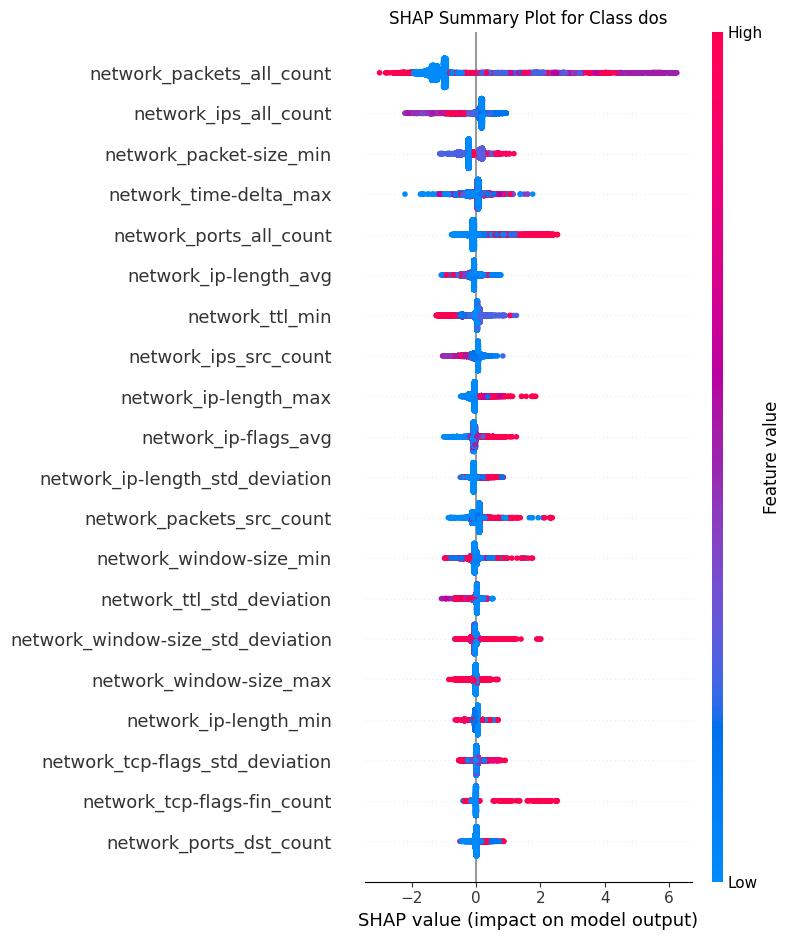
\includegraphics[width=\linewidth]{Images/xai_evaluation/shap_summary_dos.jpeg}}
			{\rule{\linewidth}{2in}}
		\caption{\texttt{dos}}
	\end{subfigure}

	\vspace{0.5em}

	\begin{subfigure}[t]{0.48\textwidth}
		\centering
		\IfFileExists{Images/xai_evaluation/shap_summary_recon.jpeg}
			{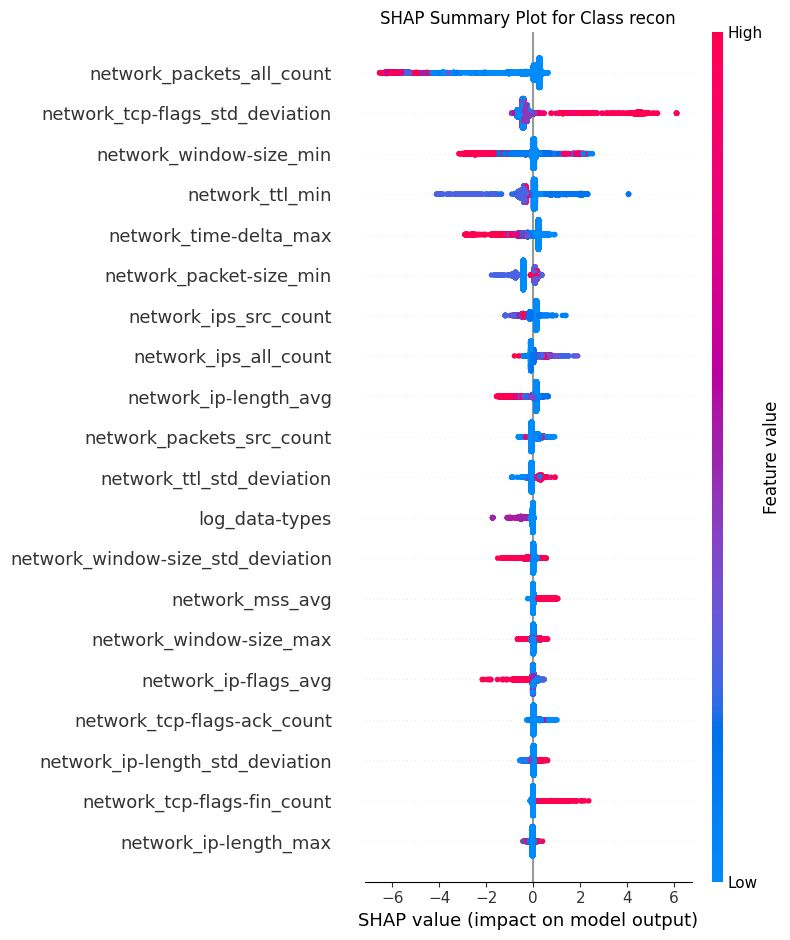
\includegraphics[width=\linewidth]{Images/xai_evaluation/shap_summary_recon.jpeg}}
			{\rule{\linewidth}{2in}}
		\caption{\texttt{recon}}
	\end{subfigure}
	\hfill
	\begin{subfigure}[t]{0.48\textwidth}
		\centering
		\IfFileExists{Images/xai_evaluation/shap_summary_malware.jpeg}
			{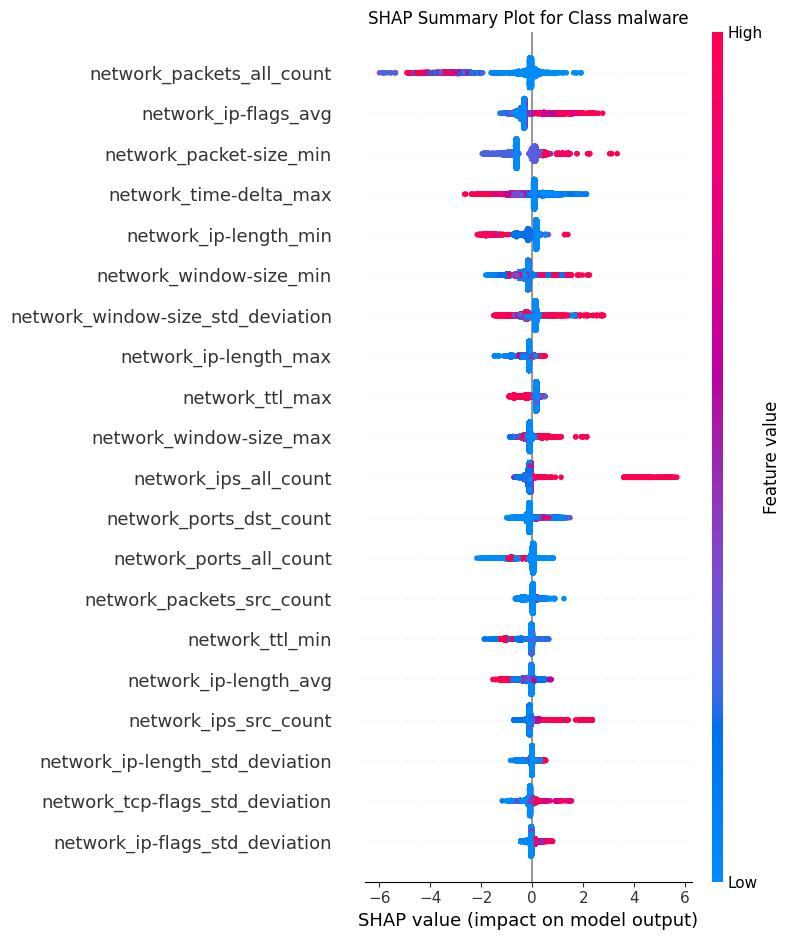
\includegraphics[width=\linewidth]{Images/xai_evaluation/shap_summary_malware.jpeg}}
			{\rule{\linewidth}{2in}}
		\caption{\texttt{malware}}
	\end{subfigure}
	\caption{SHAP summary (beeswarm) plots for the four volume-led attack classes. Long red positive tails on \texttt{network\_packets\_all\_count} across \texttt{ddos}, \texttt{dos}, \texttt{malware}, and \texttt{recon} confirm the shared volume-led direction of those classes.}
	\label{fig:xai_summary_attacks}
\end{figure}

\begin{figure}[htbp]\ContinuedFloat
	\centering
	\begin{subfigure}[t]{0.32\textwidth}
		\centering
		\IfFileExists{Images/xai_evaluation/shap_summary_bruteforce.jpeg}
			{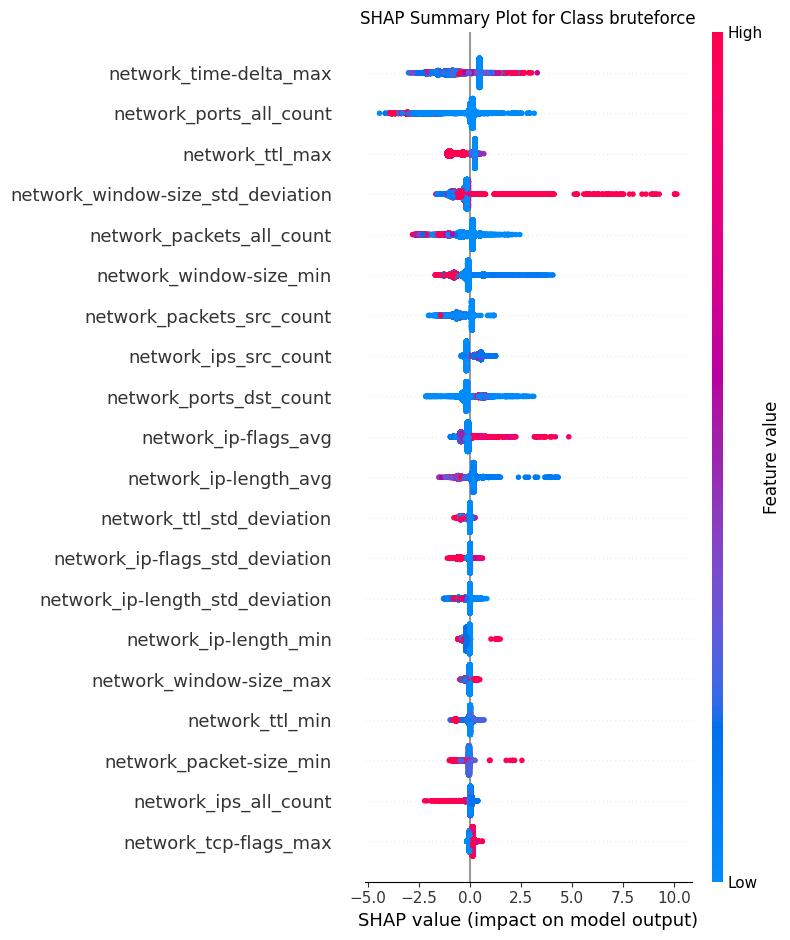
\includegraphics[width=\linewidth]{Images/xai_evaluation/shap_summary_bruteforce.jpeg}}
			{\rule{\linewidth}{2in}}
		\caption{\texttt{bruteforce}}
	\end{subfigure}
	\hfill
	\begin{subfigure}[t]{0.32\textwidth}
		\centering
		\IfFileExists{Images/xai_evaluation/shap_summary_mitm.jpeg}
			{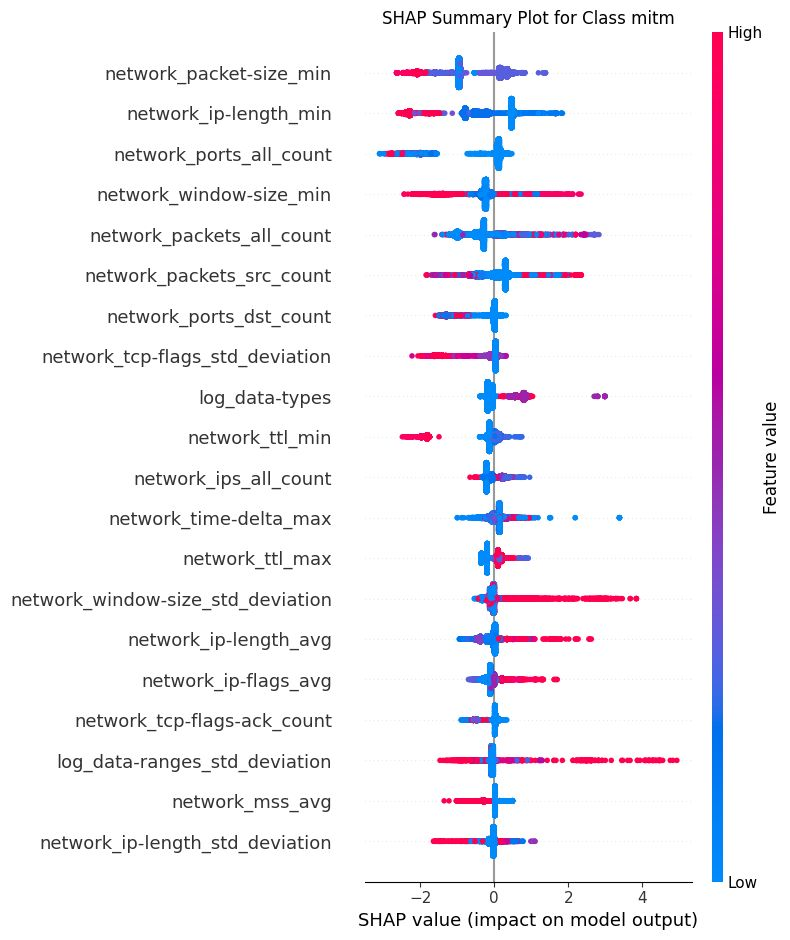
\includegraphics[width=\linewidth]{Images/xai_evaluation/shap_summary_mitm.jpeg}}
			{\rule{\linewidth}{2in}}
		\caption{\texttt{mitm}}
	\end{subfigure}
	\hfill
	\begin{subfigure}[t]{0.32\textwidth}
		\centering
		\IfFileExists{Images/xai_evaluation/shap_summary_web.jpeg}
			{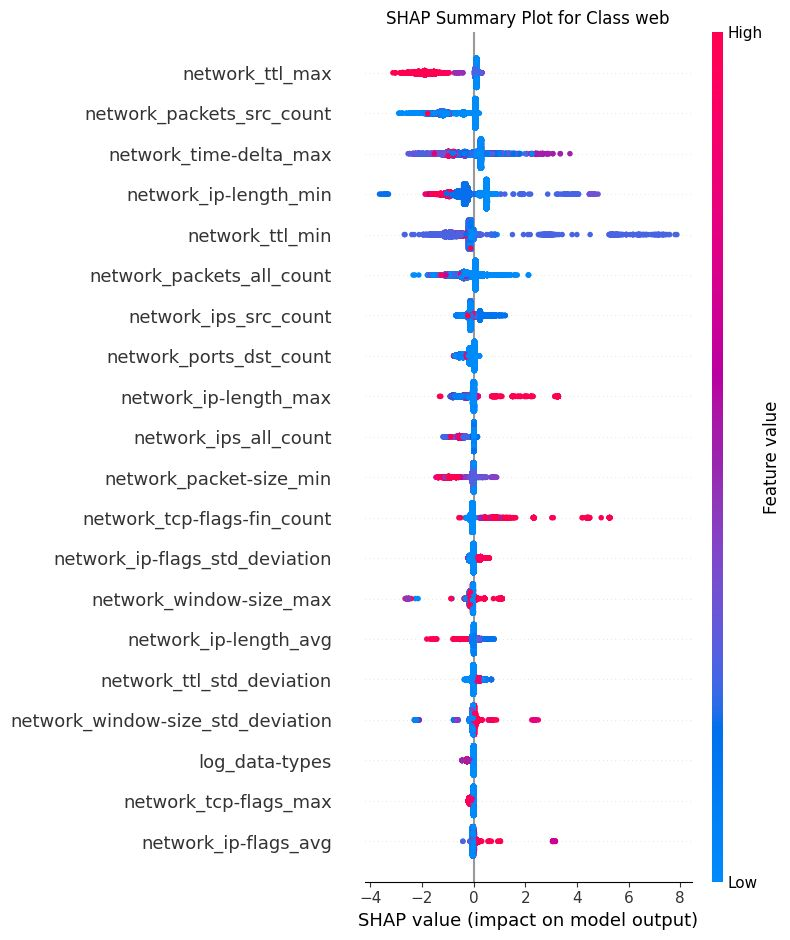
\includegraphics[width=\linewidth]{Images/xai_evaluation/shap_summary_web.jpeg}}
			{\rule{\linewidth}{2in}}
		\caption{\texttt{web}}
	\end{subfigure}
	\caption{SHAP summary (beeswarm) plots for the three distinct-signature attack classes. The visible non-linearity on top-ranked features (particularly for \texttt{mitm}) is the empirical basis for the moderate continuity score reported in Figure \ref{fig:xai_continuity}.}
	\label{fig:xai_summary_attacks_distinct}
\end{figure}

\FloatBarrier

Read together, these metrics indicate that the SHAP subsystem itself is technically sound: attributions are numerically complete, moderately stable, largely contrastive across attack families, and concentrated in a compact head that maps cleanly onto the top-3 statements the healing pipeline ingests. The only two structural concerns they surface, the \texttt{ddos}--\texttt{recon} feature overlap and the leading role of packet-level features in the \texttt{benign} decision, both point at the classifier itself rather than at the explainer, and are consistent with the accuracy findings reported earlier in this section.

\section{Multi-Agent Self-Healing Evaluation}\label{sec:mas_eval}

The true novelty of this framework lies in the autonomous self-healing loop described in Section \ref{sec:multi_agent}: a deterministic ladder engine as the primary decision path, with an LLM consulted only as a fallback. Because the classifier itself is the weak link identified in Section \ref{sec:cloud_eval}, the second round of live testing was deliberately structured to isolate the question of whether the \textit{downstream} mechanics behave correctly \textit{given} a classification that does cross the confidence gate, rather than to report an aggregate end-to-end success percentage that a broken classifier would make meaningless. Each mechanic below was exercised at least once, live, over the full HTTP-driven pipeline, and the outcome recorded as pass or fail rather than as a sampled success rate.

\begin{table}[htbp]
\caption{Self-healing mechanics verified by live, HTTP-driven testing against the full cloud pipeline.}
\label{tb:mas_results}
\centering
\begin{tabular*}{\textwidth}{@{\extracolsep{\fill}}|p{0.22\textwidth}|p{0.54\textwidth}|p{0.14\textwidth}|}
\hline
\textbf{Mechanic} & \textbf{What was exercised} & \textbf{Outcome} \\
\hline
Ladder escalation (P1$\to$P6) & Full \texttt{ddos} playbook escalation driven by simulated edge apply/verification feedback, including a scaled same-level re-apply before advancing to the next tier & Pass \\
\hline
Approval gate at P6 & \texttt{ESC-02} parking the incident in \texttt{pending\_approval}; operator approval correctly dispatching the final action and closing the incident as \texttt{human\_handoff} with an Escalation Agent-authored report & Pass \\
\hline
Benign-state decay & Decay scheduling correctly triggered after a resolution at a ladder level above 0 & Pass \\
\hline
Unhandled-attack routing & An \texttt{unhandled\_attack} classification (no configured ladder) routed directly to the Decision Agent, which retrieved grounded RAG context and selected a coherent action & Pass \\
\hline
Low-confidence-streak trigger & Decision Agent correctly consulted on the second consecutive sub-threshold classification for the same device/attack-type pairing & Pass \\
\hline
Ineffective-LLM-action handling & A Decision Agent action that verification reported as ineffective correctly triggered device isolation (\texttt{SEG-01}) and parked the incident in \texttt{awaiting\_human\_review} until explicitly resolved & Pass \\
\hline
RAG self-learning write-back & Initially found broken for the explicit-verification-feedback path (only the silent no-redetection timeout path worked); confirmed zero \texttt{learned/*.md} entries before the fix and a real entry written after it & Fixed during testing \\
\hline
\end{tabular*}
\end{table}

Every mechanic in Table \ref{tb:mas_results} passed once the classification driving it crossed the confidence gate, which is the central qualitative finding of this evaluation: the resilience-by-design argument of this framework-deterministic ladder, LLM safety net, human handoff, with a human always reachable if every automated tier is exhausted-is validated as engineering, independently of the primary classifier's real-world accuracy. The one mechanic that did not pass on first attempt, RAG self-learning write-back, illustrates why this live-testing methodology was adopted in the first place: a unit-level or code-review check would not necessarily have surfaced that the expected production feedback path (explicit edge verification) bypassed the code that records a successful decision into the retrieval corpus, whereas driving the full loop over HTTP did.

The two grouped buckets noted in Section \ref{sec:cloud_classification} as configured but unreachable, \texttt{lateral\_movement} and \texttt{exfiltration}, could not be exercised by this testing for exactly that reason: no fine-grained label the classifier can currently output maps onto either bucket, so no live classification ever reaches their playbooks. This directly resolves an inconsistency flagged in an earlier draft of this chapter, which reported a \textit{Data Exfiltration} row in this table without a corresponding playbook in Appendix \ref{app:healing_actions}; that row has been removed here, since it described a code path that, as now verified, cannot currently be reached by any classification this system produces. Reconciling the two taxonomies-either by extending the classifier's fine-grained labels to cover exfiltration and lateral-movement patterns, or by removing the two orphaned playbooks until such labels exist-is carried forward as a limitation in Section \ref{sec:limitations_integration} rather than resolved here.

\section{Cloud Dashboard: Operator-Facing Interface}\label{sec:cloud_dashboard}

The cloud tier's evaluation surface, and the intended day-to-day interface for a human operator, is a single-page web dashboard organised into six routes. Every route consumes the same live WebSocket event stream published by the cloud pipeline, so tiles, charts, and log panels all update continuously as new edge-device windows are classified and remediated. This section describes each route in turn, both to document the interface that produced the live findings reported in Sections \ref{sec:edge_eval}--\ref{sec:mas_eval} and to make it clear which parts of the framework are exposed for human oversight and which run without operator involvement.

\subsection{Overview Page}\label{sec:dash_overview}

The Overview page is the default landing route and serves as the executive summary of the entire self-healing pipeline. It is a purely read-only, real-time situational-awareness screen: it does not let the operator take any action but instead aggregates data from every other subsystem (edge ingestion, the XGBoost classifier, the LLM reporting agent, and the healing engine) into a single glanceable view.

Its key UI components are as follows.
\begin{itemize}
	\item Four KPI stat tiles: Devices Monitored (with a currently-under-attack sub-count), Windows Classified (with a flagged-as-attack sub-count), High/Critical Reports, and Healing Actions Issued.
	\item A \textit{Risk timeline} line chart plotting maximum and average classifier confidence in rolling time buckets, giving a temporal view of how risk pressure is trending across the fleet.
	\item A \textit{Severity mix} bar chart summarising LLM report counts across the Low, Medium, High, and Critical bands.
	\item An \textit{Attack type distribution} donut chart summarising XGBoost classification output plus operator and report votes across attack categories (\texttt{benign}, \texttt{ddos}, \texttt{port\_scan}, \texttt{bruteforce}, \texttt{mitm}, \texttt{unhandled\_attack}, and others).
	\item A \textit{Top devices by confidence} ranked table showing device ID, classifier confidence, attack label, severity badge, record count, and last-seen timestamp.
	\item Two live-scrolling event logs shown side by side: \textit{Recent raw ingest} (raw edge windows as they arrive) and \textit{Latest LLM reports} (natural-language incident summaries generated by the reporting LLM agent).
\end{itemize}

\begin{figure}[htbp]
	\begin{center}
		\IfFileExists{Images/cloud/cloud_operations_dashboard.jpeg}
			{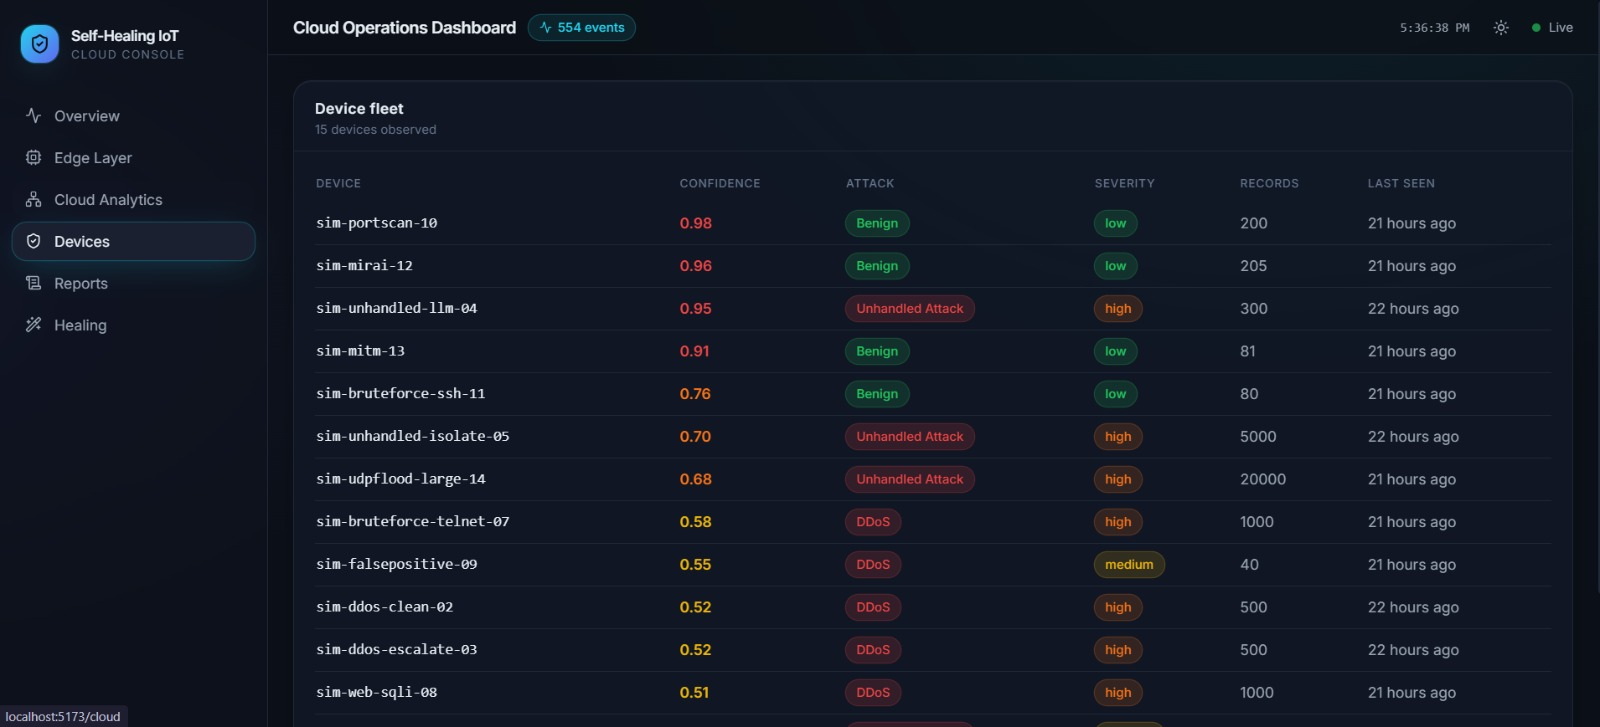
\includegraphics[width=6in]{Images/cloud/cloud_operations_dashboard.jpeg}}
			{\rule{6in}{3.5in}
			\\[-3.7cm]\centering\textit{\small [Image not yet added: Images/cloud/cloud\_operations\_dashboard.jpeg]}\\[3.5in]}
	\end{center}
	\caption{Overview page of the cloud dashboard, aggregating KPI tiles, the risk timeline, severity mix, attack-type distribution, top devices by confidence, and the raw-ingest and LLM-report live feeds into a single situational-awareness view.}
	\label{fig:dash_overview}
\end{figure}

\subsection{Edge Layer Page}\label{sec:dash_edge}

The Edge Layer page narrows the focus to the ingestion boundary of the system, the point at which raw traffic windows are received from simulated or real IoT edge devices and pushed into the XGBoost classifier. Its purpose is to let a developer or researcher validate and stress-test the edge-to-cloud pipeline in isolation, independent of the higher-level healing and reporting logic. It is the only page that contains an interactive traffic-generation control, making it the primary demonstration and testing surface of the dashboard.

Its key UI components are as follows.
\begin{itemize}
	\item Three KPI stat tiles: Raw Windows Received, Attacks Detected, and Average Classification Confidence across the observed fleet.
	\item A \textit{Confidence pressure} timeline chart tracking how the XGBoost classifier's confidence evolves over rolling five-minute windows.
	\item An embedded Edge-Layer Traffic Simulator panel with a Start/Stop control that drives a scripted 15-case test cycle (one simulated device window every approximately two minutes) through the real analytics and healing pipeline end-to-end, together with a \textit{Recent runs} log showing each simulated case as it completes.
	\item A \textit{Raw windows from edge} live log showing the \texttt{POST /api/edge/raw-ingest} payloads as they are received (device ID, record count, window duration, and timestamp).
	\item An \textit{XGBoost classifications} live log shown side by side with the raw feed, displaying the grouped label, the confidence score, and the top SHAP feature-attribution evidence for each classified window.
\end{itemize}

\subsection{Cloud Analytics Page}\label{sec:dash_cloud_analytics}

The Cloud Analytics page is a focused view of the machine-learning classification layer that runs in the cloud tier, distinct from the edge-side metrics on the Edge Layer page. Where the Edge Layer page emphasises ingestion volume and pipeline throughput, this page emphasises classification quality and outcome distribution: it answers ``what is the model finding, and how confident is it?'' rather than ``how much traffic is arriving?''.

Its key UI components are as follows.
\begin{itemize}
	\item Three KPI stat tiles: Classified Windows, Average Classifier Confidence, and Devices Monitored (distinct device IDs seen).
	\item An \textit{Attack type distribution} donut chart summarising the XGBoost classifier's output categories across the observed fleet.
	\item A \textit{Recent classifications} live log listing each classified window with device ID, predicted label and confidence score, and the SHAP feature attributions that explain the model's decision.
\end{itemize}

\begin{figure}[htbp]
	\begin{center}
		\IfFileExists{Images/cloud/cloud_analytics.jpeg}
			{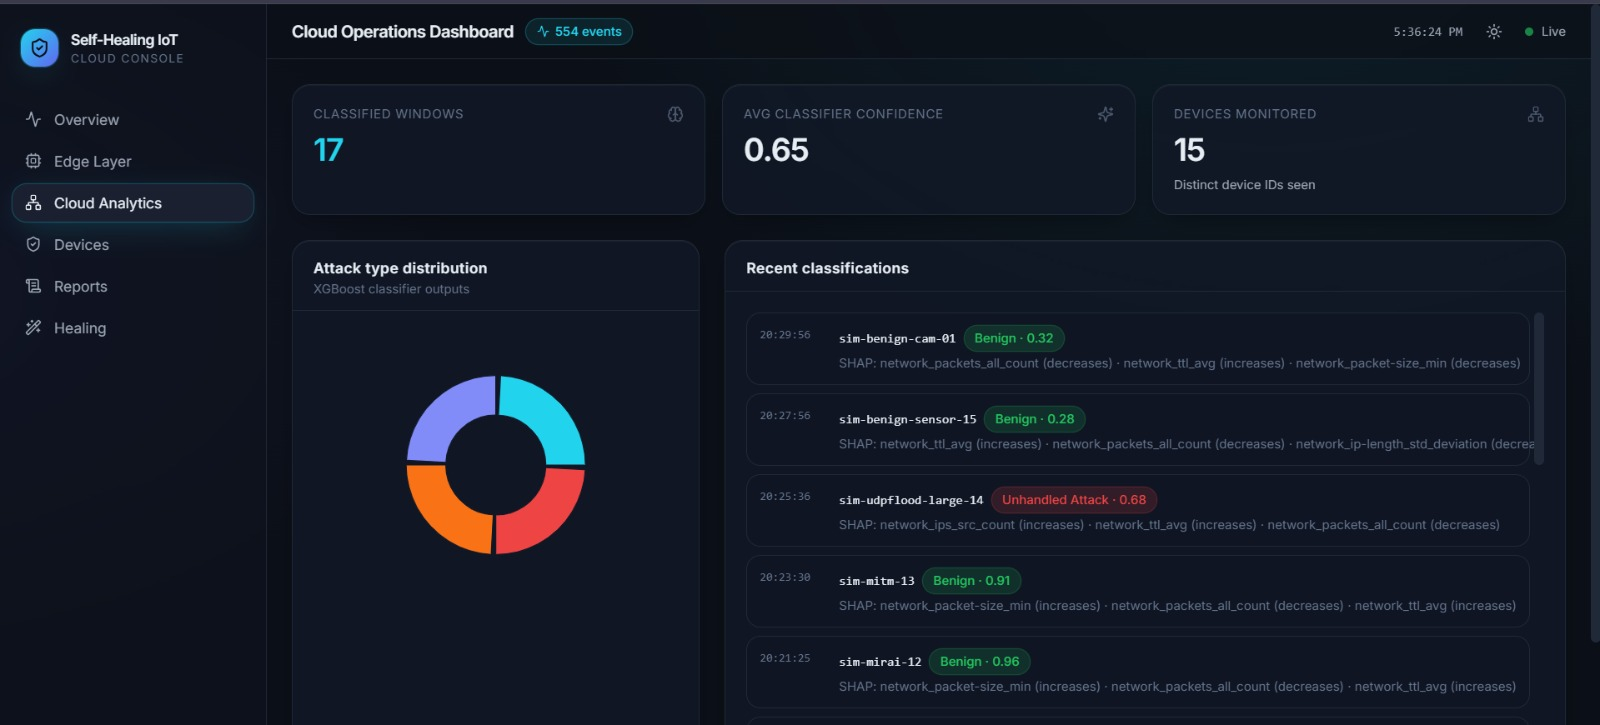
\includegraphics[width=6in]{Images/cloud/cloud_analytics.jpeg}}
			{\rule{6in}{3.5in}
			\\[-3.7cm]\centering\textit{\small [Image not yet added: Images/cloud/cloud\_analytics.jpeg]}\\[3.5in]}
	\end{center}
	\caption{Cloud Analytics page, presenting classifier-side KPIs, the attack-type distribution donut, and the recent-classifications log with per-window SHAP attributions.}
	\label{fig:dash_cloud_analytics}
\end{figure}

\subsection{Devices Page}\label{sec:dash_devices}

The Devices page provides a fleet-inventory view of every IoT device the system has observed, consolidated into a single sortable table rather than split across charts. It is the page an operator would use to look up a specific device's current risk posture, rather than to monitor system-wide trends.

Its key UI components are as follows.
\begin{itemize}
	\item A header showing the total count of observed devices (``Device fleet: $N$ devices observed'').
	\item A full device table (rendering up to 500 rows) with columns for Device ID, Confidence, Attack label (colour-coded, e.g.\ Benign, DDoS, Unhandled Attack), Severity badge (low, medium, or high), Records processed, and Last Seen timestamp.
	\item Rows colour-coded by risk: confidence values shift from green (low risk) through amber to red (high risk), and severity badges use the same low/medium/high colour language used throughout the rest of the dashboard for visual consistency.
\end{itemize}

\subsection{Reports Page}\label{sec:dash_reports}

The Reports page exposes the output of the LLM-based security reporting agent: every classified incident is summarised by the LLM into a structured natural-language report with recommended actions, and this page lets an operator browse and drill into that report history. It follows a master--detail interaction pattern, which distinguishes it from the purely passive log views on the Overview and Cloud Analytics pages.

Its key UI components are as follows.
\begin{itemize}
	\item Left panel: a scrollable, clickable list of \textit{LLM security reports}, each row showing device ID, a severity badge (low, medium, or high), the attack label, and the report timestamp.
	\item Right panel: the detail view for the selected report, showing a one-line natural-language summary; a badge row (severity, confidence score, and source engine, for example \texttt{mock} or \texttt{llm}); an \textit{Indicators} section listing the SHAP-derived signals that drove the classification (feature name, direction of influence, and SHAP value); a \textit{Recommended actions} panel with the suggested remediation, its category tag (for example \texttt{observation}), and rationale; and a raw JSON \textit{Evidence} viewer exposing the full underlying model output for auditability.
	\item User interaction: clicking any report in the left list refreshes the right-hand detail panel. This is the only page besides Healing where the user actively selects an item to inspect rather than only observing a live feed.
\end{itemize}

\begin{figure}[htbp]
	\begin{center}
		\IfFileExists{Images/cloud/reports_page.jpeg}
			{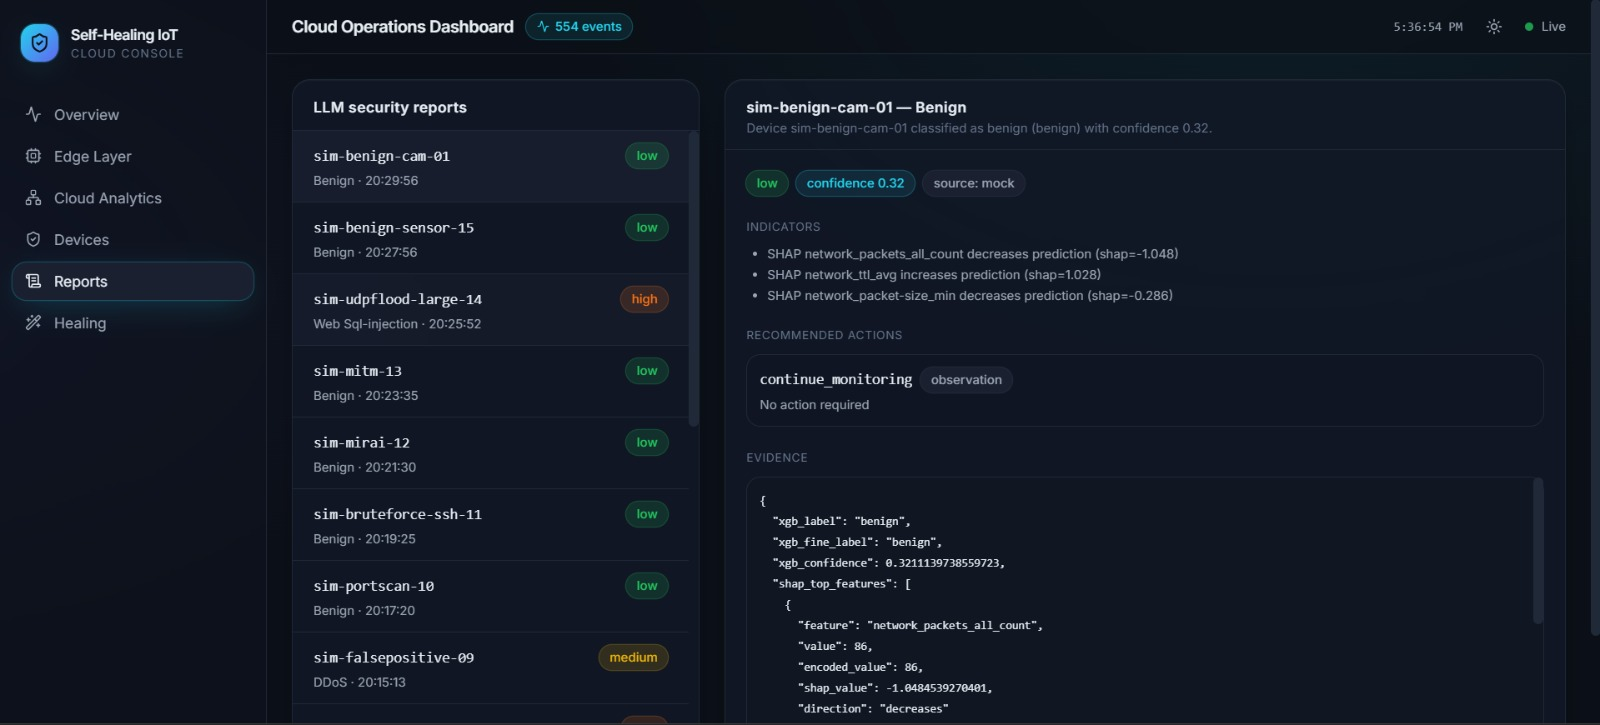
\includegraphics[width=6in]{Images/cloud/reports_page.jpeg}}
			{\rule{6in}{3.5in}
			\\[-3.7cm]\centering\textit{\small [Image not yet added: Images/cloud/reports\_page.jpeg]}\\[3.5in]}
	\end{center}
	\caption{Reports page, showing the master list of LLM-generated security reports on the left and the selected report's detail view (summary, indicators, recommended actions, and raw evidence JSON) on the right.}
	\label{fig:dash_reports}
\end{figure}

\subsection{Healing Page}\label{sec:dash_healing}

The Healing page is the operational core of the self-healing system and the most interactive page in the application. It visualises the automated incident-response workflow: a deterministic escalation ladder (P1 to P6 for network-layer responses, or B0 to B4 for device-layer responses) that attempts increasingly aggressive remediation actions, escalating to an LLM-based Decision Agent (grounded via Retrieval-Augmented Generation over a knowledge base of prior playbooks) when the deterministic ladder is exhausted or confidence is low, and finally isolating a device and handing it to a human operator when neither can resolve the incident with confidence. This page is where human-in-the-loop review and approval actually happens.

Its key UI components are as follows.
\begin{itemize}
	\item \textit{Active incidents} panel: incidents currently being remediated, each rendered as a card with status, attack-type, and device badges, and a chronological timeline of remediation attempts (ladder level, action taken, outcome, and whether the action ran in dry-run or audit mode).
	\item \textit{Resolved and handed-off} panel: closed incidents that fed back into the incident-memory store, shown with the same timeline format plus a final outcome badge (Resolved, Isolated, or Human handoff) and the resolution source (for example \texttt{via edge\_confirmed} or \texttt{via manual\_isolation\_released}).
	\item Decision Agent notes: rendered inline in an incident's timeline whenever the deterministic ladder escalates to the LLM, shown as a highlighted card with the trigger reason (for example \texttt{ladder exhausted} or \texttt{low-confidence streak}), a RAG-grounded tag, the chosen action code, a confidence percentage, and the agent's natural-language rationale for the decision.
	\item Approval Actions widget: Approve and Reject buttons shown on incidents awaiting operator sign-off before a remediation action is applied (wired to \texttt{api.approveIncident} and \texttt{api.rejectIncident}).
	\item Human Review Actions widget: for devices that have been isolated and require a human decision, three buttons are offered: \textit{Release isolation and resolve}, \textit{Handled manually}, and \textit{Escalate to permanent quarantine} (wired to \texttt{api.\allowbreak resolveHumanReview}).
	\item Operator Brief: a summary and recommendation box shown on handed-off incidents, generated by the LLM handoff agent to brief the human reviewer on what happened, what was tried, and what is recommended next (including a suggested follow-up action code).
\end{itemize}

\begin{figure}[htbp]
	\begin{center}
		\IfFileExists{Images/cloud/healing_page.jpeg}
			{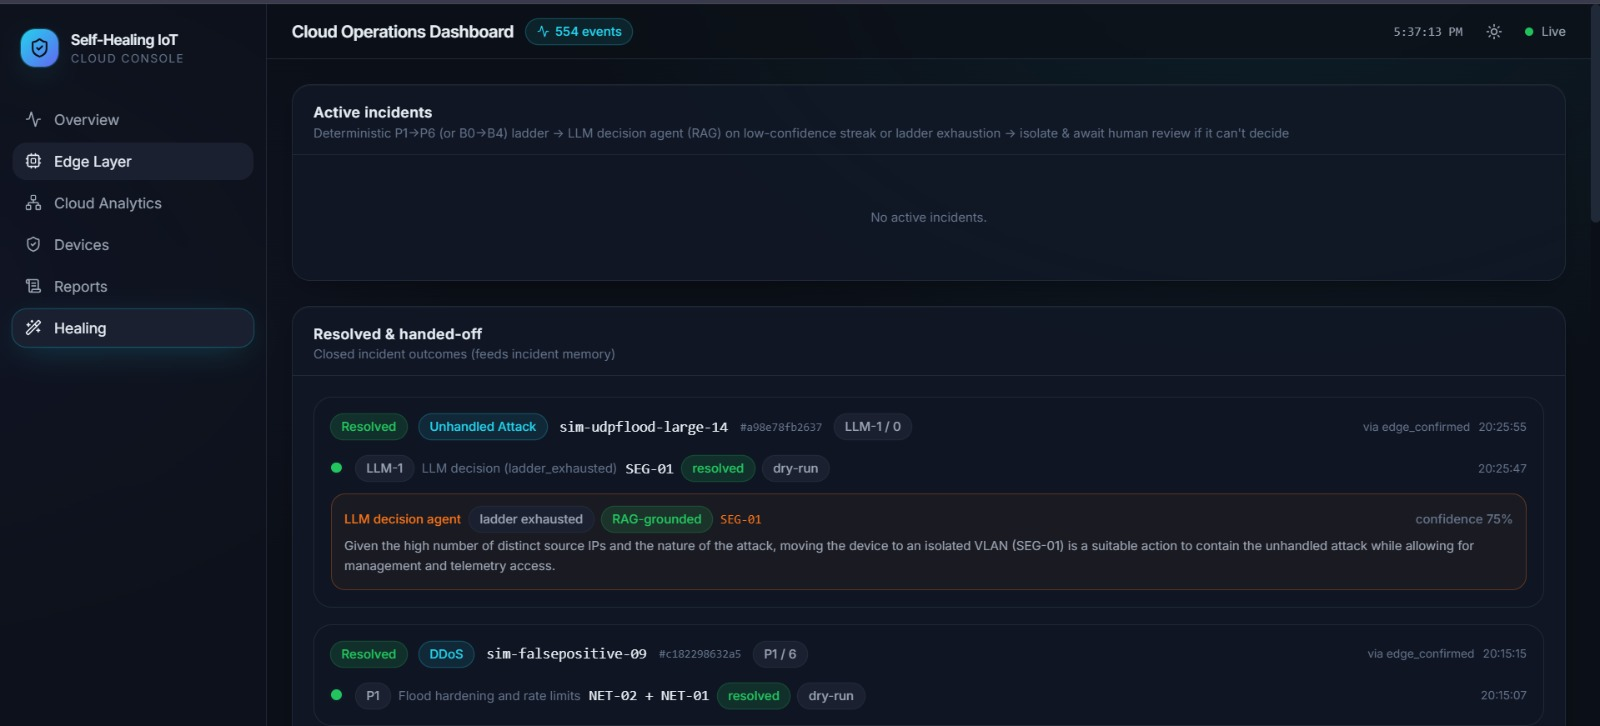
\includegraphics[width=6in]{Images/cloud/healing_page.jpeg}}
			{\rule{6in}{3.5in}
			\\[-3.7cm]\centering\textit{\small [Image not yet added: Images/cloud/healing\_page.jpeg]}\\[3.5in]}
	\end{center}
	\caption{Healing page, showing the active and resolved incident panels, inline Decision Agent notes, the approval and human-review widgets, and the LLM-generated Operator Brief on handed-off incidents.}
	\label{fig:dash_healing}
\end{figure}

\FloatBarrier

\section{Discussion}

The experimental results validate the core hypothesis of this research: a distributed, multi-stage architecture can successfully bridge the gap between lightweight anomaly detection and heavy, cognitive incident remediation in IoT networks.

\subsection{Edge Intelligence and the Mitigation of Alert Fatigue}
The superior performance of the Cascaded Hybrid Ensemble (F1-Score of 0.9971, Table \ref{tb:edge_results}) underscores the necessity of temporal awareness in IoT security. Standard static models, including the standalone Isolation Forest and standalone Deep SVDD baselines, both misclassify benign, bursty IoT telemetry as anomalous considerably more often than the fused ensemble, with standalone Deep SVDD in particular exhibiting a precision of only 53.3\% despite a comparable recall-consistent with a model that flags a great deal of benign traffic while still catching most attacks. By leveraging the GRU autoencoder to extract temporal embeddings via RMSprop optimization, the ensemble successfully captures the sequential state of the network before applying the Deep SVDD boundary. Furthermore, the Two-Stage Rolling Risk Score proved highly effective in practice. In production-like environments, security operations centers (SOCs) are often overwhelmed by transient network spikes. The rolling score acts as a low-pass filter, mathematically isolating sustained, systematic attacks from benign network jitter, effectively solving the alert fatigue problem at the edge. As discussed in Section \ref{sec:cloud_classification}, this edge-side mechanism currently operates independently of the cloud tier rather than gating what the cloud receives; Section \ref{sec:limitations_integration} discusses why.

\subsection{The Paradigm Shift to Machine-Readable XAI}
Traditionally, XAI frameworks like SHAP are designed as visualization tools for human analysts. A critical design choice in this framework is pivoting XAI to serve as a machine-to-machine interface as well: the same translated SHAP attributions that populate the Dashboard Reporting Agent's operator-facing summaries are also inserted into the prompt whenever the Decision Agent or Escalation Agent is consulted (Section \ref{sec:multi_agent}), rather than maintaining a separate, human-only explanation path. This enables whichever LLM component is invoked to reason over the specific network features that drove a classification, rather than the classification label alone, allowing for a more targeted fallback decision than a blunt default action would be. This benefit is, however, only as good as the classification being explained; Section \ref{sec:cloud_eval}'s findings on classifier accuracy apply equally to what the explainer is explaining.

\subsection{Autonomous Remediation and System Limitations}\label{sec:limitations_integration}
The multi-agent RAG pipeline demonstrated correct behaviour, mechanic by mechanic, in dynamically issuing and escalating healing commands once given a classification to act on (Table \ref{tb:mas_results}). The use of a RAG architecture successfully constrained the LLM fallback agents' outputs to physically viable commands drawn from the catalogue in Appendix \ref{app:healing_actions}, rather than free-composing network configurations that might not exist on the target device.

However, live verification testing surfaced limitations considerably more specific, and in places more serious, than could be identified from the architecture alone:

\begin{enumerate}
	\item \textbf{Classifier accuracy on real-world traffic is the framework's primary weakness, not the surrounding engineering.} Section \ref{sec:cloud_eval} documents false negatives at 90--98\% confidence, false positives that dispatched real containment against a benign device, non-monotonic confidence with attack volume, and frequently incorrect fine-grained labels even when the grouped bucket's gate is crossed. The root cause is a granularity mismatch: the classifier was trained on packet-level captures, and roughly half of its expected input features are permanently placeholder-filled because the edge layer forwards connection-log aggregates rather than packet captures. No amount of improvement to the ladder engine, the RAG grounding, or the LLM fallback agents corrects a decision made on a classification that was wrong to begin with; closing this gap requires either retraining the classifier on connection-log-derived features directly, or upgrading the edge layer's telemetry to genuinely supply the packet-level signals the current model expects.
	\item \textbf{Two of the eight configured healing playbooks are currently dead code.} \texttt{lateral\_movement} and \texttt{exfiltration} each have a full prioritised playbook in Appendix \ref{app:healing_actions}, but no fine-grained label the classifier produces maps onto either grouped bucket, so neither playbook can currently be triggered by any classification this system makes. As noted in Section \ref{sec:hybrid_ensemble}, this is at least partly explained by the training data itself: the CIC IIoT 2025 dataset's native taxonomy of 50 attack types spans seven categories (DDoS, DoS, Reconnaissance, Web, Bruteforce, MITM, and Malware/Mirai) that do not include either lateral movement or exfiltration as a category \cite{Firouzi2025}, so a classifier trained to discriminate that taxonomy has no basis for ever emitting a label that would route to either bucket. This was surfaced by, rather than hidden by, the verification process, and is recorded here as an open item rather than corrected silently.
	\item \textbf{Reliance on large cloud-based LLM APIs introduces API latency and recurring computational costs}, which may not be scalable for massively distributed micro-networks without optimization, and which is a further reason the ladder engine, rather than an LLM, is the primary decision path (Section \ref{sec:multi_agent}) rather than a secondary optimisation.
	\item \textbf{The cognitive cloud tier inherently relies on the availability of the edge-to-cloud communication link} once that link exists in a deployed sense. While the edge layer is designed to reserve bandwidth for this telemetry, a severe, distributed link-flooding attack could theoretically isolate the edge node before any healing action reaches it.
\end{enumerate}


%%%%%%%%%%%%%%%%%%%%%%%%%%%%%%%%%%%%%%%%%%%%%%%%%%%%%%%%%%%%%%%%%%%%%%%%%%%%%%%%%%%%%%%%%%%%%%%%%%
%%%%%%%%%%% END OF FILE
%%%%%%%%%%%%%%%%%%%%%%%%%%%%%%%%%%%%%%%%%%%%%%%%%%%%%%%%%%%%%%%%%%%%%%%%%%%%%%%%%%%%%%%%%%%%%%%%%%
\chapter{Conclusion and Future Work}\label{cha:conclusion}

\section{Summary of the Research}

As IoT ecosystems continue to scale and integrate into critical infrastructure, reactive and human-dependent security frameworks are no longer viable. This report presented a novel, self-healing security framework that leverages distributed intelligence to provide autonomous, closed-loop network resilience.

By pushing a cascaded hybrid GRU-Deep SVDD ensemble to the edge, the system achieves highly accurate, temporal-aware anomaly detection while maintaining a lightweight footprint. The integration of a Two-Stage Rolling Risk Score ensures that only sustained threats trigger further analysis at the edge. In the cloud tier, the framework transforms traditional black-box classification by utilizing SHAP to feed explainable telemetry into a cognitive healing pipeline: a deterministic ladder engine handles the great majority of classified incidents by escalating through a prioritised playbook, while a pair of LLM-backed agents, grounded by a RAG-enabled knowledge base, are consulted only as a fallback-for classifications the ladder cannot map to a known attack class, or for incidents that exhaust their playbook-and generate the forensic reports and human-handoff briefs that accompany every incident. This cognitive tier dynamically adjusts its strategy based on real-time edge feedback, escalating or relaxing mitigations as the evidence for an incident strengthens or resolves.

\section{Achievement of Objectives}

Section 1.3 set out five objectives for this project. Each is assessed below against the evidence gathered in Chapter~\ref{cha:results}, distinguishing what was fully achieved from what was achieved only in part.

\textbf{Objective 1-researching the feasibility of autonomic self-healing IoT security via a layered intelligence architecture-was substantively achieved.} A two-tier architecture was designed, implemented, and evaluated: a lightweight edge layer performing one-class anomaly detection and risk accumulation, and a cognitive cloud layer performing classification, explanation, and a deterministic-ladder-with-LLM-fallback healing decision. Every mechanic of that layered design passed live, HTTP-driven verification (Table 4.4), demonstrating that the layering itself-fast, local detection feeding a slower but more capable remediation tier-is a workable division of labour. The one respect in which this objective is not yet fully realised is that the two layers, as implemented, do not currently exchange data with one another in a deployed sense (Section 4.5.3); the layered architecture has been validated as a design and mechanically, but not yet as a single integrated system running end-to-end.

\textbf{Objective 2-balancing fast response with dynamic thinking to contain threats in time and sustain long-term resiliency-was partially achieved.} The deterministic ladder engine supplies the fast-response half of this objective, escalating through a prioritised playbook in a fixed, auditable order (Section 3.5), while the LLM-backed Decision and Escalation Agents supply the dynamic-thinking half for the cases the ladder cannot resolve on its own. Long-term resiliency is supported by the benign-state decay mechanism, which relaxes mitigations once a threat genuinely passes rather than leaving a device restricted indefinitely. However, Section 4.3 shows that containment ``in time'' is only as reliable as the classification that triggers it: port scans, brute-force attempts, and Mirai-style scanning traffic were classified as benign at 90--98\% confidence across every volume tested, meaning that for these attack types the fast-response path is never actually entered. The balance the objective calls for is architecturally present but not yet reliably achieved in practice for every attack class evaluated.

\textbf{Objective 3-supporting explainable and trustful decision-making through explainable AI procedures-was partially achieved.} SHAP-based feature attributions are computed for every classification and translated into structured, machine-consumable statements that are passed directly to the Dashboard Reporting Agent and, when consulted, to the Decision and Escalation Agents (Section 3.4), which is a genuine extension of XAI from a human-facing visualisation into a machine-to-machine interface. This mechanism functioned correctly wherever it was exercised. Trustworthiness, however, is undermined by the same root cause identified against Objective 2: an explanation is only as trustworthy as the decision it explains, and Section 4.3's findings on classifier accuracy-including cases where the explainer faithfully attributed a confident but incorrect classification-mean that the objective is met at the mechanism level without yet being met at the level of end-to-end decision trust.

\textbf{Objective 4-researching the use of large language models to extrapolate to previously unknown and evolving attack patterns-was achieved for the mechanism, with the caveat that it was validated against structurally unhandled classifications rather than a genuinely novel attack held out from training.} The Decision Agent, grounded by RAG over the playbooks and device-specific documentation of Appendix A, was specifically designed to be consulted when a classification falls into the \texttt{unhandled\_attack} bucket or persists at low confidence (Section 3.5), and Table 4.4 confirms that this routing worked correctly and produced a coherent, grounded action rather than a free-composed one. This demonstrates the intended extrapolation mechanism functioning as designed. What it does not yet demonstrate is extrapolation to attacks entirely outside the training distribution, since the cases exercised were drawn from the same evaluation dataset's label space rather than from a held-out, genuinely zero-day traffic pattern; this distinction is carried forward as a limitation below.

\textbf{Objective 5-creating a self-directed learning strategy for the ongoing revision of security policy-was achieved, following a defect found and corrected during evaluation.} The RAG knowledge base is designed to write every resolved incident's outcome back into its own retrieval corpus as a past action (Section 3.5), so that future incidents are grounded against an accumulating operational record rather than static playbooks alone. Live testing initially found this write-back broken for the explicit-verification-feedback path-the production path most incidents were expected to take-with only the silent no-redetection timeout path functioning; the defect was corrected during testing and confirmed via a real recorded entry (Table 4.4). With the fix in place, the self-directed learning strategy the objective calls for is in place and functioning, though it has so far been exercised only over a small number of incidents rather than validated for how policy quality evolves over a longer operational history.

Taken together, the objective most concerned with the anomaly-detection model's own accuracy and the mechanical correctness of the orchestration layer (Objectives 1, 4, and 5) were met either in full or with a narrow, clearly identified caveat; the two objectives whose fulfilment depends on the cloud-tier classifier being reliable on real-world, edge-supplied telemetry (Objectives 2 and 3) were met at the level of mechanism but not yet at the level of end-to-end trust, for the reasons documented in Section 4.3 and revisited in Section 5.4 below.

\section{Major Contributions}

This project makes the following contributions:

\begin{enumerate}
\item \textbf{A fused GRU--Deep SVDD anomaly ensemble with a quantified ablation.} Rather than presenting the hybrid model's accuracy in isolation, this report isolates and quantifies what the temporal component specifically adds over a one-class boundary method operating on point features alone (Section 4.2), giving the design choice an empirical justification beyond the architectural reasoning of Section 3.2.

\item \textbf{A two-stage, decay-based rolling risk score that treats detection as accumulating evidence rather than a single-shot decision.} The mechanism's deliberate asymmetry-risk rises faster than it decays-directly targets the alert-fatigue and transient-spike problems documented in Section 1.1.4, and is a concrete instantiation of the ``single-shot vs. persistent detection'' gap identified in Section 2.7.

\item \textbf{Repurposing SHAP as a machine-consumable interface rather than a human-facing visualisation.} Where the reviewed literature (Section 2.2) treats SHAP outputs as inputs to a human analyst's judgement, this framework serialises the same attributions into short, structured statements consumed directly by the Decision and Escalation Agents, extending explainability's role from usability aid to a precondition for automated action.

\item \textbf{A deterministic-ladder-with-LLM-fallback architecture for remediation.} Rather than delegating every healing decision to a language model, the framework reserves LLM reasoning for the specific cases a fixed, auditable playbook cannot resolve-an unhandled attack bucket or a sustained low-confidence streak-which keeps the majority of remediation decisions inspectable in advance while retaining LLM flexibility where it is actually needed. This directly addresses the diagnostic-versus-restorative gap discussed in Sections 2.3 and 2.7.

\item \textbf{A self-updating RAG knowledge base that writes its own outcomes back into its retrieval corpus.} Successful and unsuccessful healing actions are recorded as past actions alongside the static playbooks of Appendix A, so that future incidents are grounded against a growing operational record rather than fixed policy alone.

\item \textbf{A comprehensive, prioritised healing-action catalogue and playbook set (Appendix A).} The full atomic-action catalogue and its mapping into escalating, attack-specific playbooks for the classifier's grouped buckets provides a concrete, auditable enforcement vocabulary that grounds the LLM agents' outputs in physically valid actions rather than free-composed commands.

\item \textbf{A live, HTTP-driven verification methodology that surfaced defects an offline evaluation would not have.} Rather than reporting only dataset-derived metrics, Chapter~\ref{cha:results} drove the full cloud-tier pipeline end-to-end over its real interfaces, which is precisely what exposed the RAG write-back defect, the granularity mismatch between the edge's connection-log telemetry and the classifier's expected packet-level features, and the two structurally unreachable healing playbooks. This methodological choice is itself a contribution: several of the limitations reported in Section 4.5.3 are exactly the class of integration failure that a purely offline or unit-level evaluation would have missed.
\end{enumerate}

\section{Limitations}

The following limitations, most of which were surfaced directly by the live verification testing in Chapter~\ref{cha:results} rather than inferred from the architecture alone, qualify the contributions above and define the starting point for the future work in Section 5.5.

\begin{enumerate}
\item \textbf{Classifier accuracy on real-world, edge-supplied telemetry is the framework's most serious weakness.} Section 4.3 documents attacks classified as benign at 90--98\% confidence, a legitimate HTTPS session classified as a DDoS attack with real containment actions dispatched against it, classification confidence that is non-monotonic with attack volume, and fine-grained labels that are frequently wrong even when the grouped bucket's confidence gate is crossed. The underlying cause is architectural rather than a tuning defect: roughly half of the 30 features the classifier expects depend on packet-level signals the edge layer does not forward, and are populated with fixed placeholder values at inference time. No downstream component-the ladder engine, the RAG grounding, or the LLM fallback agents-can correct a decision made on an incomplete or mismatched feature vector.



\item \textbf{The framework's cloud-mediated tier is only as available as the link connecting it to the edge.} A sufficiently severe, distributed link-flooding attack could in principle isolate an edge gateway before a healing command reaches it, a risk that is independent of, and would persist even after, the transport-bridging work described in Section 5.5.





\end{enumerate}

\section{Future Research Directions}

Building on the layered edge--cloud architecture, GRU--SVDD anomaly detection, SHAP-based explanations, and multi-agent LLM orchestration presented in this work, several medium- to long-term research avenues can be identified for advancing autonomous IoT security. These directions target robustness, privacy, trustworthiness, and operational realism in large-scale deployments of self-healing IoT networks.

\subsection{Federated and Collaborative Self-Healing Across Gateways}

A first direction is to extend the proposed framework into a federated self-healing architecture where multiple IoT gateways collaboratively train anomaly-detection and threat-classification models without sharing raw telemetry. Recent work on federated IDS for IIoT has shown that distributed training can achieve accuracy close to centralized systems while preserving data privacy and improving scalability, suggesting that integrating FedAvg, FedProx, or attention-weighted aggregation into the GRU--SVDD and XGBoost components could make the self-healing pipeline resilient to heterogeneous traffic and non-IID data distributions.

\subsection{Hybrid AI--Blockchain Trust and Audit for Healing Actions}

A second avenue is the exploration of hybrid AI--blockchain architectures in which healing actions, model updates, and operator overrides are recorded on lightweight distributed ledgers to provide tamper-evident audit trails and cross-domain trust. Recent surveys on FL-based IDS and decentralized cybersecurity frameworks highlight blockchain as a promising foundation for secure data provenance and device authentication in autonomous IoT ecosystems, and coupling the orchestrator's decisions with on-chain verification could help balance extensive automation with regulatory and compliance requirements.

\subsection{Reinforcement and Meta-Learning for Adaptive Healing Policies}

Third, the rule-based healing catalogue can be evolved into a reinforcement-learning or meta-learning layer that continuously optimizes remediation policies under changing attack patterns, resource constraints, and business priorities. Studies on self-healing cybersecurity systems recommend leveraging deep reinforcement learning and meta-learning to adapt control strategies over time, suggesting that the framework's risk score and SHAP attributions could be used as state signals and rewards for agents that learn when to isolate, throttle, or reconfigure services while respecting safety and service-level objectives.

\subsection{Constrained Multi-Agent LLM Security Orchestration}

A fourth direction is to formalize the multi-agent LLM core using constrained decision-making and optimization techniques that explicitly separate stochastic plan generation from deterministic enforcement, reducing the risk of unsafe or conflicting actions. Recent multi-agent security systems propose architectures where LLM agents generate candidate mitigation portfolios while an optimization or rule-engine layer enforces closed-world action validity and resource feasibility, and adapting such self-adaptive pattern-selection schemes to IoT self-healing could strengthen runtime guarantees without sacrificing the flexibility of agentic reasoning.

\subsection{Dataset-Centric Evaluation and Real-World Benchmarking}

Fifth, future work should focus on dataset-centric evaluation and real-world benchmarking of the self-healing pipeline across multiple contemporary IoT security datasets and realistic testbeds. Recent studies emphasize that federated and edge-native IDS must be assessed on heterogeneous datasets and deployment scenarios to uncover drift, robustness issues, and performance gaps, indicating that systematic experiments on Edge-IIoTset, CIC-IoT2023, TON-IoT, and emerging mission-critical IoT environments would be essential for validating the generalizability of the proposed GRU--SVDD, XGBoost--SHAP, and multi-agent LLM stack.

\subsection{Safety, Explainability, and Human-in-the-Loop Assurance}

Finally, the integration of safety-aware design, explainable AI, and human-in-the-loop assurance mechanisms should be deepened beyond current SHAP-based explanations and operator escalation. Recent trustworthy IDS frameworks combine global and local explanations with adversarial hardening and continual replay to turn explanations into robustness actions, and extending this idea to the self-healing pipeline---by systematically linking explanatory artifacts to healing options and operator dashboards---could improve analyst trust, regulatory acceptance, and safe deployment in critical IoT infrastructures.

\section{Publications and Research Outcomes}

At the time of writing, no results from this project have been published or submitted to a peer-reviewed venue. The project budget (Table 3.3) reserves funding for a conference paper registration fee, reflecting the group's intention to prepare a submission distilling the cascaded GRU--Deep SVDD ensemble and its evaluation once the integration limitations identified in Section 5.4-most notably the edge-cloud transport bridge and the classifier's feature-granularity mismatch-have been addressed and the framework has been demonstrated end-to-end on the target edge hardware rather than through the test-harness-mediated verification reported in this report. A concrete submission target and timeline will be finalised once this remaining integration work is complete.

%%%%%%%%%%%%%%%%%%%%% Appendices %%%%%%%%%%%%%%%%%%%%%
\appendix
\chapter{Healing Action Catalogue and Prioritised Remediation Playbooks}\label{app:healing_actions}

This appendix documents the full policy content referenced in Section \ref{cha:methodology} as part of the Knowledge Base \& RAG System that the Decision and Escalation Agents query when an incident cannot be resolved by the deterministic path alone. Section \ref{app:catalogue} lists the atomic healing actions available to the gateway, grouped by mechanism. Section \ref{app:playbooks} then shows how the Ladder Engine composes these atomic actions into a prioritised, escalating playbook for each attack class the cloud-tier classifier can output, plus the benign case in which no attack is present at all. Together, these two tables are the concrete substance behind the four abstract action categories introduced in Figure \ref{fig:architecture} (VLAN isolation, bandwidth allocation, port blocking, and local response actions): every entry in the playbooks below resolves to one or more rows of the catalogue, and every row of the catalogue maps onto one of those four categories or the observation/escalation functions that support them.

\section{Healing Action Catalogue}\label{app:catalogue}

Table \ref{tab:healing_catalogue} lists every atomic action the gateway can execute, organised into seven functional groups: network and traffic control (\texttt{NET}), segmentation and Layer-2 integrity (\texttt{SEG}, \texttt{L2}), access/credential/session control (\texttt{ACC}), service and application-layer control (\texttt{SVC}), device recovery (\texttt{DEV}), observation and forensics (\texttt{OBS}), and escalation (\texttt{ESC}). Each ID is referenced directly in the playbooks of Section \ref{app:playbooks}; a playbook priority tier that lists, for example, ``\texttt{NET-02 + NET-01}'' is invoking both of those catalogue entries together as a single combined step.

\begin{longtable}{|p{0.10\textwidth}|p{0.16\textwidth}|p{0.20\textwidth}|p{0.415\textwidth}|}
\caption{Healing action catalogue: every atomic action available to the Pi 5 gateway, grouped by mechanism.}
\label{tab:healing_catalogue}\\
\hline
\textbf{ID} & \textbf{Group} & \textbf{Action} & \textbf{Mechanism on the Pi 5 gateway} \\
\hline
\endfirsthead
\multicolumn{4}{c}{\tablename\ \thetable{} -- continued from previous page}\\
\hline
\textbf{ID} & \textbf{Group} & \textbf{Action} & \textbf{Mechanism on the Pi 5 gateway} \\
\hline
\endhead
\hline \multicolumn{4}{r}{\textit{Continued on next page}}\\
\endfoot
\hline
\endlastfoot
NET-01 & Network and traffic control & Adaptive rate limiting & Per-source token-bucket / connection-rate limit on the gateway firewall for the offending 5-tuple or source. \\
\hline
NET-02 & Network and traffic control & Flood-specific hardening & SYN cookies, half-open connection caps, conntrack table limits, ICMP/UDP rate caps. \\
\hline
NET-03 & Network and traffic control & Temporary source block & Drop/blackhole the attacking source address with an escalating TTL (5 $\rightarrow$ 15 $\rightarrow$ 60 min). \\
\hline
NET-04 & Network and traffic control & Port / protocol block & Close the abused destination port or protocol at the gateway for that device. \\
\hline
NET-05 & Network and traffic control & Probe and scan filtering & Drop unsolicited SYN/FIN/NULL/Xmas probes and ICMP sweeps; suppress port-unreachable replies. \\
\hline
NET-06 & Network and traffic control & Egress and C2 blocking & Deny outbound to the observed command-and-control endpoint; DNS sinkhole the domain on the local resolver. \\
\hline
NET-07 & Network and traffic control & Aggregate source block & Block the offending prefix / subnet when many sources share it, instead of thousands of single rules. \\
\hline
NET-08 & Network and traffic control & Traffic shaping & Fair-queue and cap the victim device's share of uplink so the flood cannot starve neighbouring devices. \\
\hline
SEG-01 & Segmentation and L2 integrity & Quarantine VLAN & Move the device to an isolated VLAN that reaches only the gateway (management and telemetry only). \\
\hline
SEG-02 & Segmentation and L2 integrity & MAC-level block & Drop frames from the offending MAC at the bridge; deauthenticate / disassociate the wireless client. \\
\hline
SEG-03 & Segmentation and L2 integrity & Full isolation & Deny all traffic to and from the device except the controller heartbeat channel. \\
\hline
L2-01 & Segmentation and L2 integrity & ARP truth restoration & Install static ARP bindings for gateway and device; broadcast corrective gratuitous ARP; flush poisoned caches. \\
\hline
L2-02 & Segmentation and L2 integrity & ARP / DHCP inspection & Enable dynamic ARP inspection and DHCP snooping; drop offers from any non-authorised server. \\
\hline
L2-03 & Segmentation and L2 integrity & Force encrypted channel & Reject plaintext HTTP / MQTT / DNS for that device; pin traffic to TLS and to the gateway's DoT resolver. \\
\hline
L2-04 & Segmentation and L2 integrity & Re-key and re-provision & Rotate PSK, re-issue device certificate, invalidate key material that may have been observed. \\
\hline
ACC-01 & Access, credentials, sessions & Progressive source ban & Ban the source after N failed authentications with exponential back-off (jail-style rule set). \\
\hline
ACC-02 & Access, credentials, sessions & Target account lockout & Lock or throttle the specific account being guessed rather than the whole service. \\
\hline
ACC-03 & Access, credentials, sessions & Credential rotation & Force a new admin password / API token / MQTT credential for the device and its gateway record. \\
\hline
ACC-04 & Access, credentials, sessions & Harden authentication surface & Disable Telnet and password login, enforce key or certificate auth, restrict management ports to a gateway allowlist. \\
\hline
ACC-05 & Access, credentials, sessions & Session and token revocation & Kill active sessions, invalidate cookies and bearer tokens, force re-authentication. \\
\hline
SVC-01 & Service and application layer & Service restart & Restart the affected daemon on the device or its gateway-side proxy to clear exhausted resources. \\
\hline
SVC-02 & Service and application layer & Process kill and persistence removal & Terminate the malicious process and remove its persistence (init entry, cron job, watchdog respawn). \\
\hline
SVC-03 & Service and application layer & Virtual patch / WAF rule & Insert a reverse-proxy rule at the gateway blocking the observed payload class (injection, traversal, upload abuse). \\
\hline
SVC-04 & Service and application layer & Disable exposed function & Turn off the vulnerable endpoint, remote web UI, UPnP, or other non-essential service. \\
\hline
SVC-05 & Service and application layer & Request hygiene & Tighten body size, header and timeout limits; enforce strict input validation at the proxy. \\
\hline
DEV-01 & Device recovery & Network stack restart & Bounce the device's interface and re-DHCP without a full reboot. \\
\hline
DEV-02 & Device recovery & Graceful reboot & Reboot via device API or SSH; clears memory-resident state. \\
\hline
DEV-03 & Device recovery & Hard power cycle & Toggle the smart plug, PoE port or GPIO relay feeding the device when it is unresponsive. \\
\hline
DEV-04 & Device recovery & Golden-config restore & Push the last known-good configuration snapshot held by the gateway. \\
\hline
DEV-05 & Device recovery & Factory reset and re-provision & Reset to factory defaults, then re-provision inside quarantine with fresh unique credentials. \\
\hline
DEV-06 & Device recovery & Firmware re-flash / rollback & Re-flash a signed known-good image, or roll back to the previous verified version. \\
\hline
OBS-01 & Observation and forensics & Extended capture & Start full packet capture and verbose host logging for the incident window (evidence; always parallel). \\
\hline
OBS-02 & Observation and forensics & Honeypot / tarpit redirect & Redirect the attacker's flows to a deception service to profile behaviour without exposing the real device. \\
\hline
OBS-03 & Observation and forensics & Sensitivity boost & Lower the detection threshold and shorten the inference window for this device temporarily. \\
\hline
OBS-04 & Observation and forensics & Baseline update & Fold confirmed-benign behaviour back into the device profile / incremental model. \\
\hline
ESC-01 & Escalation & Operator notification & Dashboard alert plus out-of-band message with the incident timeline and the actions already tried. \\
\hline
ESC-02 & Escalation & Permanent quarantine & Keep the device isolated pending manual review; block automatic release. \\
\hline
ESC-03 & Escalation & Incident report & Generate machine- and human-readable reports, including the peer-device sweep results. \\
\hline
\end{longtable}

\section{Prioritised Healing-Action Playbooks}\label{app:playbooks}

For each attack class the cloud-tier classifier (Section \ref{cha:methodology}) can output, the Ladder Engine retrieves a playbook of the form shown below: a sequence of priority tiers, ordered from least disruptive (attempted first) to most disruptive (attempted only once cheaper tiers have failed), plus, where applicable, a parallel track of observation and forensics actions (denoted \texttt{P-par}) that run alongside the priority ladder rather than as a step within it. This ordering is what the ``iterate strategy'' loop in Figure \ref{fig:multiagent} steps through: each time verification reports that a dispatched action was not effective, the Ladder Engine advances to the next priority tier for the same attack class rather than repeating the tier that already failed or jumping directly to the most disruptive option.

\subsection{Benign}

The benign playbook (Table \ref{tab:playbook_benign}) is the counterpart, at the remediation layer, to the risk-score decay mechanism described in Section \ref{cha:methodology} (Equation \ref{e:risk_decay}): as a device's risk score relaxes toward its baseline, tier B2 relaxes any standing mitigations in step, rather than leaving a device quarantined or rate-limited indefinitely after the threat that triggered it has genuinely passed.

\begin{longtable}{|p{0.10\textwidth}|p{0.13\textwidth}|p{0.18\textwidth}|p{0.465\textwidth}|}
\caption{Benign playbook: tiers B0--B4.}
\label{tab:playbook_benign}\\
\hline
\textbf{Priority} & \textbf{Action ID(s)} & \textbf{Action name} & \textbf{What is done on/for the device} \\
\hline
\endfirsthead
\multicolumn{4}{c}{\tablename\ \thetable{} -- continued from previous page}\\
\hline
\textbf{Priority} & \textbf{Action ID(s)} & \textbf{Action name} & \textbf{What is done on/for the device} \\
\hline
\endhead
\hline \multicolumn{4}{r}{\textit{Continued on next page}}\\
\endfoot
\hline
\endlastfoot
B0 & - & No action & Continue passive monitoring. No firewall, service or device change of any kind. \\
\hline
B1 & OBS-04 & Close open incidents & If an incident is open for this device and Benign persists for the full window, mark the last executed action as successful at level $k$ and record $k$ in the effectiveness statistics. \\
\hline
B2 & - & Decay and roll back mitigations & After the hold time, relax standing mitigations one step at a time: release TTL blocks, lift rate limits, return the device from the quarantine VLAN, restore the original rule set from the snapshot. \\
\hline
B3 & OBS-04 & Baseline maintenance & Fold the confirmed-benign window into the per-device behavioural profile; retrain or update the incremental model on a schedule, never during an open incident. \\
\hline
B4 & - & Integrity self-check & Verify the gateway's own rule set matches the intended state, confirm log shipping works, and confirm golden config and firmware images are present and valid. \\
\hline
\end{longtable}

\newpage \subsection{DDoS}

\begin{longtable}{|p{0.10\textwidth}|p{0.13\textwidth}|p{0.18\textwidth}|p{0.465\textwidth}|}
\caption{DDoS playbook: priority tiers P1--P6 plus the parallel observation track.}
\label{tab:playbook_ddos}\\
\hline
\textbf{Priority} & \textbf{Action ID(s)} & \textbf{Action name} & \textbf{What is done on/for the device} \\
\hline
\endfirsthead
\multicolumn{4}{c}{\tablename\ \thetable{} -- continued from previous page}\\
\hline
\textbf{Priority} & \textbf{Action ID(s)} & \textbf{Action name} & \textbf{What is done on/for the device} \\
\hline
\endhead
\hline \multicolumn{4}{r}{\textit{Continued on next page}}\\
\endfoot
\hline
\endlastfoot
P1 & NET-02 + NET-01 & Flood hardening and rate limits & Enable SYN cookies, cap half-open connections and conntrack entries, apply per-source connection-rate and packet-rate limits at the gateway. Stateless; protects the device without dropping legitimate sessions. \\
\hline
P2 & NET-03 + NET-05 & Block top talkers & Rank sources by contribution over the window and blackhole the top offenders with a 15 min TTL; apply protocol-specific filtering for the observed vector. \\
\hline
P3 & NET-07 + NET-08 & Aggregate block and shaping & Collapse per-address rules into prefix-level blocks; fair-queue and cap the victim's uplink share so other IoT devices behind the Pi keep working. \\
\hline
P4 & SEG-01 & Quarantine VLAN for the victim & Move the device to the isolated VLAN so the flood no longer reaches it; it stays reachable from the gateway for telemetry and control. \\
\hline
P5 & DEV-02 $\rightarrow$ DEV-03 & Reboot, then power cycle & Graceful reboot while still quarantined to clear exhausted state; hard power cycle if it does not return or is unresponsive to the API. \\
\hline
P6 & SEG-03 + ESC-01/02/03 & Isolate and hand over & Hold full isolation, notify the operator with the timeline of everything tried, generate the incident report. No further automated action. \\
\hline
P-par & OBS-01 + OBS-03 & Capture and fleet sensitivity & Full capture from first confirmation; raised sensitivity on all sibling devices, since a flood against one node often coincides with recon or infection attempts against the rest. \\
\hline
\end{longtable}

\subsection{DoS}

\begin{longtable}{|p{0.10\textwidth}|p{0.13\textwidth}|p{0.18\textwidth}|p{0.465\textwidth}|}
\caption{DoS playbook: priority tiers P1--P6 plus the parallel observation track.}
\label{tab:playbook_dos}\\
\hline
\textbf{Priority} & \textbf{Action ID(s)} & \textbf{Action name} & \textbf{What is done on/for the device} \\
\hline
\endfirsthead
\multicolumn{4}{c}{\tablename\ \thetable{} -- continued from previous page}\\
\hline
\textbf{Priority} & \textbf{Action ID(s)} & \textbf{Action name} & \textbf{What is done on/for the device} \\
\hline
\endhead
\hline \multicolumn{4}{r}{\textit{Continued on next page}}\\
\endfoot
\hline
\endlastfoot
P1 & NET-01 + NET-02 & Rate limit the source & Per-source token bucket on the abused port plus a connection-count cap for that source. Reversible, no effect on other peers. \\
\hline
P2 & NET-03 & Temporary source block & Blackhole the source with an escalating TTL: 5 min first occurrence, 15 min on repeat, 60 min on a third within the hour. \\
\hline
P3 & SVC-01 + SVC-05 & Restart the exhausted service, tighten limits & Restart the affected daemon to release leaked sockets, threads and memory; tighten timeouts, max body size and per-client concurrency at the gateway proxy. \\
\hline
P4 & NET-04 (+ SVC-04) & Close the abused port / protocol & Block the targeted port at the gateway for this device, exposing only what it genuinely needs; disable the exposed function if non-essential. \\
\hline
P5 & DEV-01 $\rightarrow$ DEV-02 $\rightarrow$ DEV-04 & Recover the device & Restart the network stack first (cheapest), then a full reboot, then restore the golden configuration if the device returns misconfigured. \\
\hline
P6 & SEG-01 + ESC-01 & Quarantine and escalate & Quarantine, alert the operator with the resource-exhaustion evidence, recommend a firmware or vendor-side fix. \\
\hline
P-par & OBS-01 + OBS-03 & Capture and sensitivity & Full capture; sensitivity boost on the affected device only (unlike DDoS, no fleet-wide boost needed). \\
\hline
\end{longtable}

\subsection{Reconnaissance}

\begin{longtable}{|p{0.10\textwidth}|p{0.13\textwidth}|p{0.18\textwidth}|p{0.465\textwidth}|}
\caption{Reconnaissance playbook: priority tiers P1--P6.}
\label{tab:playbook_recon}\\
\hline
\textbf{Priority} & \textbf{Action ID(s)} & \textbf{Action name} & \textbf{What is done on/for the device} \\
\hline
\endfirsthead
\multicolumn{4}{c}{\tablename\ \thetable{} -- continued from previous page}\\
\hline
\textbf{Priority} & \textbf{Action ID(s)} & \textbf{Action name} & \textbf{What is done on/for the device} \\
\hline
\endhead
\hline \multicolumn{4}{r}{\textit{Continued on next page}}\\
\endfoot
\hline
\endlastfoot
P1 & OBS-01 + OBS-03 & Observe silently, raise sensitivity & Full capture of the scan, extract the source fingerprint and target list, lower detection thresholds for every device the scan touched. No blocking yet. \\
\hline
P2 & NET-05 & Filter probes, reduce leakage & Drop unsolicited SYN/FIN/NULL/Xmas probes and ICMP sweeps, suppress port-unreachable and TTL-expired replies, normalise responses so open and closed ports look alike. \\
\hline
P3 & NET-01 & Rate limit / tarpit the scanner & Cap new connections per second from that source and delay responses so a full scan becomes prohibitively slow without an outright block. \\
\hline
P4 & NET-03 + SVC-04 & Block the source, shrink the surface & Block the scanner for 30 min and permanently disable the non-essential exposed services it found (remote web UI, UPnP, Telnet, debug ports); apply the hardened config snapshot if one exists. \\
\hline
P5 & OBS-02 or SEG-01 & Deceive (external) or quarantine (internal) & External source: redirect its flows to a honeypot/tarpit while the real device is untouched. Internal source: the scanning device is presumed compromised - quarantine it and enter the Malware (Mirai) playbook. \\
\hline
P6 & ESC-01 + ESC-03 & Alert and report & Notify the operator that reconnaissance is sustained and targeted, attach the target/port map, recommend a segmentation review, sweep peers for the same indicators. \\
\hline
\end{longtable}

\subsection{Web}

\begin{longtable}{|p{0.10\textwidth}|p{0.13\textwidth}|p{0.18\textwidth}|p{0.465\textwidth}|}
\caption{Web playbook: priority tiers P1--P6.}
\label{tab:playbook_web}\\
\hline
\textbf{Priority} & \textbf{Action ID(s)} & \textbf{Action name} & \textbf{What is done on/for the device} \\
\hline
\endfirsthead
\multicolumn{4}{c}{\tablename\ \thetable{} -- continued from previous page}\\
\hline
\textbf{Priority} & \textbf{Action ID(s)} & \textbf{Action name} & \textbf{What is done on/for the device} \\
\hline
\endhead
\hline \multicolumn{4}{r}{\textit{Continued on next page}}\\
\endfoot
\hline
\endlastfoot
P1 & SVC-03 + SVC-05 & Virtual patch at the gateway proxy & Insert a rule blocking the observed payload class (injection strings, traversal sequences, oversized or unexpected uploads) and tighten body, header and method limits. Device firmware unchanged. \\
\hline
P2 & ACC-05 + ACC-01 & Revoke sessions, ban the source & Invalidate active sessions and tokens for the interface (any hijacked session dies), then ban the source after N blocked attempts. \\
\hline
P3 & SVC-04 & Disable the exposed interface & Turn off the vulnerable endpoint, or restrict the whole web UI to gateway-local access, keeping the device's primary function running. \\
\hline
P4 & ACC-03 + ACC-04 & Rotate credentials, harden auth & Assume the interface leaked or accepted something: rotate admin credentials and API tokens, enforce key/certificate auth, disable password login, re-check the account list for additions. \\
\hline
P5 & DEV-04 + SVC-01 & Restore known-good state & Push the golden configuration snapshot, restart the web service, re-verify the integrity baseline - with the device in quarantine so it cannot be re-hit mid-restore. \\
\hline
P6 & DEV-06 / ESC-02 & Re-flash or retire & Re-flash a signed known-good firmware image (operator approval), re-provision with fresh credentials, then report. If re-flash is impossible, hold permanent quarantine. \\
\hline
\end{longtable}

\subsection{Brute Force}

\begin{longtable}{|p{0.10\textwidth}|p{0.13\textwidth}|p{0.18\textwidth}|p{0.465\textwidth}|}
\caption{Brute Force playbook: priority tiers P1--P6.}
\label{tab:playbook_bruteforce}\\
\hline
\textbf{Priority} & \textbf{Action ID(s)} & \textbf{Action name} & \textbf{What is done on/for the device} \\
\hline
\endfirsthead
\multicolumn{4}{c}{\tablename\ \thetable{} -- continued from previous page}\\
\hline
\textbf{Priority} & \textbf{Action ID(s)} & \textbf{Action name} & \textbf{What is done on/for the device} \\
\hline
\endhead
\hline \multicolumn{4}{r}{\textit{Continued on next page}}\\
\endfoot
\hline
\endlastfoot
P1 & ACC-01 & Progressive source ban & Ban the source after N failures with exponential back-off (5 failures $\rightarrow$ 5 min, then 30 min, then 24 h). Cheapest possible action; defeats most automated guessing. \\
\hline
P2 & ACC-02 + NET-03 & Lock the account, block the source & Throttle or lock the specific account being guessed rather than the whole service, and blackhole the source addresses with a 60 min TTL. \\
\hline
P3 & ACC-04 + NET-04 & Remove the guessable surface & Disable Telnet entirely, disable password authentication in favour of keys/certificates, restrict management ports to the Pi 5 gateway allowlist. \\
\hline
P4 & ACC-05 + ACC-03 + SEG-01 & Treat as compromise & Kill all active sessions, rotate every credential and key on the device and in the gateway record, and move the device to the quarantine VLAN. \\
\hline
P5 & DEV-02 + DEV-04 & Reboot and restore & Reboot inside quarantine to clear memory-resident payloads, then restore the golden configuration and re-verify the account list and authorised keys. \\
\hline
P6 & DEV-05 + ESC-03 & Factory reset and re-provision & Factory reset (operator approval), then re-provision inside quarantine with fresh unique credentials, key-only authentication and Telnet permanently disabled. \\
\hline
\end{longtable}

\subsection{MITM}

\begin{longtable}{|p{0.10\textwidth}|p{0.13\textwidth}|p{0.18\textwidth}|p{0.465\textwidth}|}
\caption{MITM (Man-in-the-Middle) playbook: priority tiers P1--P6.}
\label{tab:playbook_mitm}\\
\hline
\textbf{Priority} & \textbf{Action ID(s)} & \textbf{Action name} & \textbf{What is done on/for the device} \\
\hline
\endfirsthead
\multicolumn{4}{c}{\tablename\ \thetable{} -- continued from previous page}\\
\hline
\textbf{Priority} & \textbf{Action ID(s)} & \textbf{Action name} & \textbf{What is done on/for the device} \\
\hline
\endhead
\hline \multicolumn{4}{r}{\textit{Continued on next page}}\\
\endfoot
\hline
\endlastfoot
P1 & L2-01 & Restore correct ARP mappings & Install static ARP bindings for the gateway and affected devices, flush poisoned caches, broadcast corrective gratuitous ARP so victims relearn the authentic MAC. \\
\hline
P2 & L2-02 & Enable inspection, reject rogue infrastructure & Turn on dynamic ARP inspection and DHCP snooping on the bridge; drop DHCP offers and DNS responses not from the authorised service; pin the device resolver to the Pi. \\
\hline
P3 & SEG-02 & Remove the attacker from the segment & Block the offending MAC at the bridge and, for wireless clients, deauthenticate/disassociate it. If the MAC belongs to a known internal device, treat that device as compromised. \\
\hline
P4 & L2-03 & Make interception worthless & Reject plaintext protocols for the affected devices: enforce TLS for HTTP and MQTT, force DNS over TLS to the gateway resolver, drop downgrade attempts. \\
\hline
P5 & L2-04 + ACC-03 & Re-key everything exposed & Rotate PSKs, re-issue device certificates, rotate any credential or token that traversed the intercepted path, invalidate sessions established during the incident window. \\
\hline
P6 & SEG-03 + ESC-01/03 & Isolate the segment and escalate & Isolate the affected segment, alert the operator with spoofing evidence and the list of possibly exposed secrets, recommend port security and 802.1X. \\
\hline
\end{longtable}

\subsection{Malware (Mirai)}

\begin{longtable}{|p{0.10\textwidth}|p{0.13\textwidth}|p{0.18\textwidth}|p{0.465\textwidth}|}
\caption{Malware (Mirai) playbook: priority tiers P1--P6 plus the parallel observation track.}
\label{tab:playbook_mirai}\\
\hline
\textbf{Priority} & \textbf{Action ID(s)} & \textbf{Action name} & \textbf{What is done on/for the device} \\
\hline
\endfirsthead
\multicolumn{4}{c}{\tablename\ \thetable{} -- continued from previous page}\\
\hline
\textbf{Priority} & \textbf{Action ID(s)} & \textbf{Action name} & \textbf{What is done on/for the device} \\
\hline
\endhead
\hline \multicolumn{4}{r}{\textit{Continued on next page}}\\
\endfoot
\hline
\endlastfoot
P1 & SEG-01 + NET-06 & Contain and cut command-and-control & Immediately move the device to the quarantine VLAN and block egress to the observed C2 endpoint (address block plus DNS sinkhole). Stops C2 control and the device's participation in outbound floods and scanning. \\
\hline
P2 & SVC-02 & Kill the process and remove persistence & Terminate the malicious process and its watchdog, remove persistence (init/rc entries, cron, spurious units, modified startup scripts), close the ports it opened. \\
\hline
P3 & DEV-02 $\rightarrow$ DEV-03 & Reboot / power cycle inside quarantine & Reboot to clear the memory-resident payload; hard power cycle if unresponsive. Stays in quarantine across the reboot. \\
\hline
P4 & ACC-04 + ACC-03 & Close the infection vector & Before release: disable Telnet (23/2323) and password SSH permanently, replace every default or shared credential with a unique one, enforce key/certificate auth, restrict management to the gateway allowlist. \\
\hline
P5 & DEV-04 $\rightarrow$ DEV-06 & Rebuild from a trusted image & Restore the golden configuration; if integrity checks still fail, re-flash a signed known-good image or roll back to the last verified version. Performed entirely inside quarantine. \\
\hline
P6 & DEV-05 / ESC-02 + ESC-03 & Reset, or retire under quarantine & Factory reset and re-provision with fresh unique credentials (operator approval), or keep the device permanently quarantined pending replacement. Generate the report and sweep every peer device. \\
\hline
P-par & OBS-01 + OBS-03 & Capture, fleet sensitivity, credential audit & Capture including the full C2 conversation and any dropper transfer; sensitivity boost on all devices; immediate credential audit of every device sharing the compromised credential set. \\
\hline
\end{longtable}

%%%%%%%%%%%%%%%%%%%%% Bibiliography %%%%%%%%%%%%%%%%%%%%%
\cleardoublepage
\bibliographystyle{ieeetr}
\refstepcounter{chapter}
\addcontentsline {toc}{chapter}{\bibname}
% _____Add Bibiliography using BibTex file_____
\bibliography{bibliography}

\end{document}